%  $Description: Thesis
%  $Author: Dipanwita Guhathakurta $
%  $Date: 1 March 2022  $
%  $Revision: 1.0 $

\documentclass[11pt]{book}
\usepackage{style/iiit_thesis}

\usepackage{hyperref}
\usepackage{times}
\usepackage{epsfig}
\usepackage{amsmath}
\usepackage{listings}
\DeclareMathOperator*{\argmax}{argmax}
\usepackage{amssymb}
\usepackage{latexsym}
\usepackage{multirow}
\usepackage{algorithm}
% \usepackage{algorithm2e}
\usepackage{caption}
\usepackage{braket}
\usepackage{float}
\usepackage{newfloat}
\usepackage{xtab}
\usepackage{longtable}
\usepackage{xcolor}
\usepackage{color}
\usepackage{url,lineno,microtype,subcaption}
% \usepackage[onehalfspacing]{setspace}
\usepackage{natbib}
\newtheorem{remark}{Remark}
\usepackage{graphicx}
% \usepackage{subcaption}
\usepackage{mwe}
%\usepackage{changepage}
\usepackage{tabularx}
\usepackage{multicol, blindtext}
%\usepackage{algpseudocode}
% \usepackage{algorithm}

\long\def\symbolfootnote[#1]#2{\begingroup%
\def\thefootnote{\fnsymbol{footnote}}\footnote[#1]{#2}\endgroup}
\renewcommand{\baselinestretch}{1.2}
\onecolumn
%--------------------------------------------------------

\begin{document}
\pagenumbering{roman}

%% TITLE PAGE
\thispagestyle{empty}
\begin{center}
\vspace*{1.5cm}
{\Large \bf Discrete and Continuous Trajectory Optimization Methods for Complex Robot Systems}

\vspace*{3.75cm}
{\large Thesis submitted in partial fulfillment\\}
{\large  of the requirements for the degree of \\}

\vspace*{1cm}
{\it {\large Master of Science \\ in \\ \textbf{Electronics and Communication Engineering} \\ by Research}\\}
    

\vspace*{1cm}
{\large by}

\vspace*{5mm}
{\large Dipanwita Guhathakurta\\}
{\large 2018112004\\
{\small \tt dipanwita.g@research.iiit.ac.in}}


\vspace*{4.0cm}
{\psfig{figure=figures/iiit.eps,width=14mm}\\}
{\large International Institute of Information Technology\\}
{\large Hyderabad - 500 032, INDIA\\}
{\large March, 2023\\}
\end{center}

%% COPYRIGHT PAGE
\newpage
\thispagestyle{empty}
\renewcommand{\thesisdedication}{{\large Copyright \copyright~~Dipanwita Guhathakurta, 2023\\}{\large All Rights Reserved\\}}
\thesisdedicationpage

%% CERTIFICATE PAGE
\newpage
\thispagestyle{empty}
\vspace*{1.5cm}
\begin{center}
{\Large International Institute of Information Technology\\}
{\Large Hyderabad, India\\}
\vspace*{3cm}
{\Large \bf CERTIFICATE\\}
\vspace*{1cm}
\noindent
\end{center}
It is certified that the work contained in this thesis, titled 
``Discrete and Continuous Trajectory Optimization Methods for Complex Robot Systems'' 
by Dipanwita Guhathakurta, has been carried out under
my supervision and is not submitted elsewhere for a degree.

\vspace*{3cm}
\begin{tabular}{cc}
\underline{\makebox[1.5in]{}} & \hspace*{5cm} \underline{\makebox[2.5in]{}} \\
\today & \hspace*{5cm} Adviser: Prof. K. Madhava Krishna
\end{tabular}
\oneandhalfspace

\vspace*{3cm}
\begin{tabular}{cc}
\underline{\makebox[1.5in]{}} & \hspace*{5cm} \underline{\makebox[2.5in]{}} \\
\today & \hspace*{5cm} Co-Adviser: Prof. Arun Kumar Singh
\end{tabular}
\oneandhalfspace

%%% DEDICATION PAGE
\newpage
\thispagestyle{empty}
\renewcommand{\thesisdedication}{One Small Step for Robot, One Giant Leap for Mankind}{\large }
\thesisdedicationpage

\mastersthesis
\renewcommand{\baselinestretch}{1.5}

% ACKNOWLEDGEMENTS PAGE
\chapter*{Acknowledgements}
\label{ch:ack}
I wish to express my gratitude to my adviser, Prof. K. Madhava Krishna from the Robotics Research Centre at IIIT Hyderabad, for being a huge pillar of support, from helping me recognize my aptitude for research to allowing me to hone my skills in multiple sub-domains under Robotics. I am also immensely thankful to my co-adviser, Prof. Arun Kumar Singh from the University of Tartu, Estonia, for guiding me in every step of my research journey, starting from formulating research problems to hands-on pair programming. I would also like to thank Prof. Ponnurangam Kumaraguru for boosting my confidence in research paper writing and allowing me to explore diverse domains during my Independent Study under his supervision.

Next, I would like to thank the faculty at IIIT Hyderabad for providing rigorous training in mathematics and Electronics at the undergraduate level that helped me build my foundations in Robotics. I owe my understanding of Robotics to the project-based electives taught by Prof. Harikumar Kandath, Prof. K. Madhava Krishna, and Prof. Spandan Roy and to the Robotics Summer School organized by my seniors. 


I would also like to convey my gratitude to Fatemeh Rastgar, a Junior Ph.D. Researcher under Prof. Singh, who has supported me as a mentor, helping me gain a strong understanding of multi-robot planning algorithms and GPU-acceleration libraries. My teammates in the manipulator project from RRC - Vishal Reddy Mandadi, Md. Nomaan Qureshi, Bipasha Sen, Aditya Aggarwal, and Kallol Saha have also played a significant role in my understanding of physics simulators and Reinforcement Learning-based robot control. My student mentors - Mithun Babu Nallana, Jyotish P, and Raghu Ram Theerthala, helped me take my first steps in robot path planning at the end of my second year and patiently reviewed my implementations of state-of-the-art algorithms. In addition, my batchmates and fellow research students at RRC have often readily contributed suggestions to improve my research work and validated my ideas. Aditya Sharma Meduri has helped me get acquainted with ROS and Gazebo to run simulations for my paper. My batchmates and friends, Vedant Mundheda, Karan Mirakhor, Rahul Swayampakula, Nipun Wahi and Manav Bhatia have constantly offered their feedback on my research projects as teammates in course projects and external competitions. They have also supported me throughout my degree, helping me balance my academics with research, along with my social life on campus.

Finally, I would like to thank my mother and grandmother for constantly supporting me and believing in me. 


%% ABSTRACT PAGE
\chapter*{Abstract}
\label{ch:abstract}
Path planning for autonomous systems is a fundamental problem in robotics, especially when the task assigned to a robot is heavily dependent on the motion of one or more of its constituent parts. Efficient path planning requires fast adaptation to changes in the environment and generalizability to a variety of tasks while ensuring the kinematic and dynamic constraints of the robot and its workspace are respected. Present-day planning algorithms for robots fail to achieve real-time performance for complex systems such as multi-robot systems and multi-jointed robot manipulators. In fact, the path planning objectives for these complex systems often present mathematical infeasibilities when posed as an optimization problem or become computationally cumbersome to compute by pure sampling. Further, these algorithms do not generalize to the task of collision avoidance against a wide variety of obstacles for multi-robot systems with a large number of robots or robots with high-dimensional articulation. The primary focus of this dissertation is to present computationally-tractable solutions to the trajectory optimization problem for both multi-robot systems and manipulators. We explore gradient-based and stochastic optimization techniques and perform mathematical reformulations to adapt them to a wide variety of applications.

First, we provide the requisite background in robot path planning, including robot kinematics, trajectory representation methods, and collision-avoidance techniques. We also discuss state-of-the-art methods in gradient-based trajectory optimization and stochastic trajectory optimization. Next, we present a distributed GPU-based multi-agent trajectory optimizer that first converts the gradient-based multi-agent trajectory optimization problem into a set of simple matrix-matrix products and then leverages parallel computations over GPUs to accelerate these computations. We demonstrate through a large number of qualitative and quantitative experiments in simulation that our distributed algorithm outperforms existing sequential trajectory optimizers or sampling-based methods for multi-robot planning. Next, we design a collision-aware path planner for robot manipulators operating in the high-dimensional joint space and demonstrate its application across scenes with different types and numbers of obstacles. We finally couple this stochastic optimization-based path planner with a low-level controller for the task of pushing objects on a table using a robot manipulator. We also make our software for multi-agent path planning public for open-source development so that our algorithm can be used for further research in this domain.


\tableofcontents
\listoffigures
\listoftables

%--------------------------------------------------------

\chapter{Introduction}
\label{ch:intro}
\section{Scope of the Thesis}

The task of path planning for a robot involves finding an optimal start-to-goal trajectory that enables autonomous intelligent motion. A path planning algorithm for an autonomous robot performs the task of a pilot operating an aircraft, first understanding the environment, then estimating a high-level path from its start to destination and, finally, deciding on the controls necessary to execute this path. It must be aware of the dynamic and hardware constraints associated with the robot mechanical system, while interacting heavily with its environment and adapting its motion to potential changes in its surroundings. The ability of drones, autonomous cars and personal robots to maneuver through complex environments relies on the following components as depicted in Fig \ref{fig:intro_overview_robot}:

\begin{figure}[ht]
    \centering
    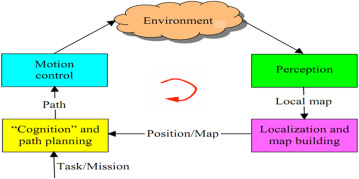
\includegraphics{figures/intro/overview_robot.jpg}
    \caption[Overview of Autonomous Robot Systems]{An overview of the components of an autonomous robot system. The perception component gathers data from the environment and sends a local map to the robot for detecting its own pose, which is eventually sent into the task/path planning module. The planned path or task sequence is finally sent for execution to the low-level motion controller. \textit{Source: \cite{overview_robot}}}
    \label{fig:intro_overview_robot}
\end{figure}

\begin{enumerate}
    \item A data ingestion system, consisting of a fusion of sensors (camera, LiDAR, Infrared Sensors) that form the sensory system of the robot, allowing it to interact with its surroundings. 
    \item A localization system that allows the robot to map its environment and calibrate its own pose with respect to it.
    \item\label{item:global-planning} A global path planner that returns a high-level path from the start to destination, similar to Google Maps planning the shortest route between two cities.
    \item\label{item:local-planning} A low-level motion controller that interacts with the underlying robot control system and plans a sequence of controls, such as linear and angular velocity, that executes the high-level plan.
\end{enumerate}

The focus of this thesis is to address points \ref{item:global-planning} and \ref{item:local-planning} for complex robot systems.

\subsection{Research problems Tackled}

Solving the high-level path-planning problem introduces the challenge of representing a start-to-goal robot trajectory efficiently. To put it simply, a trajectory should define a sequence of predefined points or a function mapping successive timestamps to the robot motion space. For fixed-base robots, such as tabletop manipulators, the trajectory needs to be planned for its moving components, i.e. the joints and the end-effector. The optimality of a trajectory is determined by several heuristics that will be discussed in Section \ref{sec:traj_eval_metrics} as well as the ability to avoid collisions with obstacles in the environment. Mathematically, finding the optimal trajectory can be represented as an optimization problem with a predefined task-based objective function, collision avoidance constraints, kinematic and dynamic bounds, and boundary constraints. 


In this thesis, we explore novel approaches to solve the trajectory optimization problem in high-dimensional spaces for interaction-aware robot systems. Broadly, we tackle the following research problems:

\begin{enumerate}\label{enum:problems-addressed-by-thesis}
    \item[\textbf{T1}] \textit{To accelerate robot trajectory computation for adaptive path planning}

    For robots continuously interacting with the environment, generating an offline path to be followed by the controller in the future may not guarantee optimal motion. The robot should be able to adapt its trajectory with respect to changes in the environment, which necessitates repeated re-computation of the trajectory optimization problem. It is, therefore, important to accelerate the optimizer for online re-planning while also equipping the robot itself with predictive models for potential changes in the environment. For instance, an individual quadrotor in a drone swarm would need to update its trajectory plan by predicting the trajectories of the other drones, or a self-driving car would re-compute its route in an online setting based on traffic predictions. We target to achieve real-time generation of start-to-goal robot trajectories to allow for online adaptive path planning and demonstrate mathematical techniques that allow this computational acceleration.
    

    \item[\textbf{T2}] \textit{To design real-time path planning frameworks for multi-robot systems}\label{intro:multi-robot_aim}

    The path planning problem for multi-robot systems requires us to repeat the core per-robot trajectory optimization over multiple agents while considering interactions among the robots as well as with the environment. For each robot, the other robots in the system can be thought of as dynamic obstacles. Collision avoidance between a pair of robots involves predicting each other's trajectories or communicating their current states continuously. The system-wide optimization problem eventually becomes intractable with an increase in the number of robots. We attempt to parallelize trajectory computation for multi-robot systems in batches and accelerate the per-batch optimization through fast matrix operations over GPUs and approximations of collision constraints.

    \item[\textbf{T3}] \textit{To extend trajectory optimization methods for motion planning in robots with complex dynamics, such as manipulators}

    For complex dynamical systems, such as multi-jointed robot manipulators, the trajectory is planned in the high-dimensional joint space or in the end-effector space, governed by strict kinematic constraints. The high dimensionality of solution spaces and the complexity of dynamic and kinematic constraints makes continuous-time trajectory optimization computationally expensive and slow. We adopt a discrete-time path-planning approach, sample points from a distribution in the solution space to guess candidate trajectories and simulate them to intelligently update the sample distribution along the optimization iterations. 
    
\end{enumerate}

\section{Motivation}

This section discusses the inspiration behind some of the methods discussed in the subsequent chapters of this dissertation. We present the challenges that arise in solving the path-planning problem for multi-robot systems and multi-jointed robot manipulators and discuss the limitations of existing approaches.

\subsection{GPU-Accelerated Distributed Multi-Robot Trajectory Optimization}

The problem of coordination planning between multiple robots in robot fleets or drone swarms has been tackled through two optimization paradigms in literature:

\begin{itemize}
    \item \textit{Centralized Optimization}, where the trajectories of all robots are computed together. An implicit ordering is maintained among the robots for sequentially optimizing their trajectories, where each robot avoids collision by using the optimal trajectories of other robots computed before it. This sequential solution to the multi-robot planning problem has been depicted in Figure \ref{fig:intro_sequential_optimization}.

    \begin{figure}
    \centering
    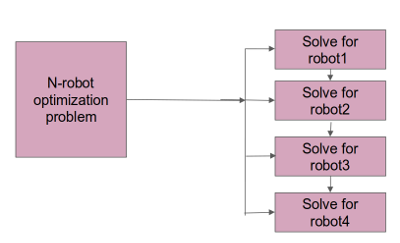
\includegraphics[scale=0.5]{figures/intro/sequential-planning-pipeline.png}
    \caption[Sequential Planning Pipeline for Multi-Robot Systems]{For sequential optimization, an implicit ordering is maintained among the robots, and each robot uses the trajectories of other robots computed before it to compute the collision avoidance constraints while planning its own path. }
    \label{fig:intro_sequential_optimization}
\end{figure}

    For joint optimization, the system-wide trajectory planning is performed simultaneously as a single large-optimization problem returning trajectories for all the robots in one go. The optimization is performed over the larger feasible solution space, involving trajectory variables for all the robots together. 
    \item \textit{Distributed Optimization}, where the trajectory planning problem of each robot is completely decoupled from the other robots. Each robot makes predictions about the others' trajectories based on a prediction model to compute collision-free paths. That is, for an $n$-robot system, each robot considers $n-1$ collision constraints with other robots while planning its trajectory. The per-robot optimization problem becomes simpler to solve and this is repeated over all $n$ robots.
\end{itemize}

Centralized optimization approaches, whether sequential or joint, discussed in \cite{chen2015decoupled}, \cite{incremental_scp_how}, fail to scale efficiently with an increase in the number of robots in the system. The pairwise collision avoidance constraints among the robots scale quadratically with the number of robots. Distributed approaches, on the other hand, are fast to compute paths but susceptible to digressions between the trajectory predictions and actual robot trajectories and have been shown in \cite{dmpc_carlos} to be less effective in collision avoidance. 

To achieve our goal discussed in \ref{intro:multi-robot_aim} of real-time trajectory planning for multiple robots, we choose the distributed optimization paradigm owing to its speed. We aim to achieve computational acceleration on the following two fronts:

\begin{enumerate}
    \item \label{motivation: per_robot} Speeding up the per-robot trajectory optimization 
    \item \label{motivation:parallelization} Avoiding having to loop over all robots while computing individual paths by parallelizing decoupled trajectory computations.
\end{enumerate}

To achieve \ref{motivation: per_robot}, we approximate the trajectory optimization problem as a sequence of matrix operations so that effectively we only need to solve a set of linear equations to obtain the trajectory of each robot. We then vectorize our computations and solve the planning problem for all robots by stacking up independent per-robot problems into a large block matrix. This removes the need to loop over an increasing number of robots and returns trajectories for all robots in a single shot. We cache computationally expensive operations such as block matrix inversing through clever mathematical reformulations of the optimization problem and leverage GPUs to accelerate matrix multiplications. We also compare our approach against a diverse range of state-of-the-art multi-robot path planners and achieve a 2x computational acceleration while not compromising on other metrics such as collisions and trajectory length, as will be shown in Section \ref{sec: GPU_mat_Results}.

\subsection{Stochastic Trajectory Optimization for Robot Manipulators}


Path planning for robot manipulators involves planning a sequence of controls to achieve a desired objective, for example, pushing an object from one point to another or picking and placing an object at a target location. Stochastic Trajectory Optimization is an optimization technique used to generate optimal trajectories for robot manipulators. The STO algorithm optimizes the control inputs of a robot to minimize a cost function that captures the desired task objectives using a probabilistic approach.
It generates a large number of random trajectories and evaluates their cost function values. It then selects the best-performing trajectories and generates new random trajectories around them to further explore the search space. This process is repeated until a satisfactory solution is found.

The STO algorithm is particularly useful for manipulator path planning since it can work with high-dimensional motion spaces and non-differentiable and discontinuous cost functions, It is also robust to uncertainties and disturbances in the environment and sensor noise, which gives it advantages in complex and uncertain planning tasks over gradient-based optimizers. 

In chapter \ref{ch:bl_arm}, we use a version of STO to plan collision-free trajectories for robot manipulators in both the joint-angle space and the Cartesian end-effector space. We design a novel cost function, incorporating collision penalty, joint limit cost, and trajectory length. We then combine our STO planner with a low-level controller for non-prehensile tasks, such as pushing an object on a tabletop from a start position to a desired goal position. 



\section{Thesis Layout}

\begin{itemize}
    \item[C1] This is the introductory chapter, which discusses the scope of the work carried out in this thesis in terms of global and local path planning, addresses the research problems we are tackling and outlines the motivation behind some of the methods we have adopted to solve them.
    \item[C2] In this chapter, we present a background of standard algorithms used for continuous-time and discrete-time trajectory optimization for individual robots that form a necessary prerequisite to understand the ideas discussed in the following chapters. We also discuss two primary paradigms in trajectory optimization - gradient-based optimization and sampling-based optimization, and compare their applications in complex robot systems.
    \item[C3] We present the first contribution of this thesis - Fast Joint Multi-Robot Trajectory Optimization by GPU Accelerated Batch Solution of Distributed Sub-Problems. This algorithm employs mathematical reformulations to allow efficient caching of gradients and convex approximations for collision constraints in multi-robot systems and computes trajectories in near real-time for as many as 36 robots.
    \item[C4] This chapter presents the second contribution of this thesis - a sampling-based trajectory optimization framework for global path planning and its application in designing a bi-level push planner for robot manipulators. We test and show the efficacy of our optimizer in complex tabletop rearrangement scenarios for a few common robot manipulators.
    \item[C5] We conclude with a summary of methods and results discussed in this thesis and the scope of extension of this work in the future.
\end{itemize}


%--------------------------------------------------------

\chapter{Gradient-based and Sampling-based Trajectory Optimization}
\label{ch:background}
This chapter introduces some fundamental background concepts that are essential for understanding the methods adopted in the subsequent chapters.

We first discuss the differences in kinematics among different types of robots and the necessity of designing a suitable trajectory representation respecting these differences prior to formulating a path planning problem. We talk about continuous-time trajectory representation using Cubic Splines and Bernstein polynomials, which are leveraged extensively in both our GPU-based multi-robot optimizer and the bi-level manipulator optimizer. Next, we introduce how to pose a trajectory optimization problem and explore two broad types of optimization - Gradient-based and Sampling-based. We contrast the performance of these two paradigms for various applications and then explore collision avoidance constraints to the trajectory optimization problem. Under standard collision avoidance techniques, we discuss two approaches - distance-based Collision Avoidance, and Time-scaling. We also coin a few standard evaluation metrics for judging the quality of a trajectory planned by an optimizer.

Next, we discuss Multi-Robot Path Planning, starting with real-world multi-agent systems and the challenges involved in extending standard path planning approaches directly to them. We analyze a few existing multi-robot path planners and discuss their advantages and weaknesses. Finally, we provide a brief introduction to batch trajectory optimization and commercial off-the-shelf GPU-based mathematical libraries to prime the reader for the next chapter on our GPU-accelerated optimizer.

Next, we move on to the path planning and motion planning for robot manipulators and discuss state-of-the-art optimization methods used for manipulator planning. We offer a detailed explanation of methods such as CHOMP\cite{CHOMP}, TrajOpt\cite{TrajOpt}, STORM\cite{STORM} and Cross-Entropy Methods(CEM)\cite{iCEM}. These optimization techniques form the backdrop for the Via-Point Stochastic Trajectory Optimization(VP-STO)\cite{VP-STO} method, which forms a crucial component in our bi-level optimization framework for push actions in manipulators.

\section{Mobile Robot Kinematics}

Kinematics equations dictate how given a set of controls, the state of a robot changes. Thus if a robot starts at a given state, its kinematics will tell us what will be the robot state if a set of controls are executed. These kinematic laws are specific to the design and motion of the robot. Broadly, mobile robots (those in which a full-body displacement occurs during motion) can be classified into the following two types based on their kinematics:

\subsection{Holonomic Robots}\label{sec:holonomic_robots}

For a robot with $n$ controllable degrees of freedom, it is considered holonomic if it is capable of moving in any of those $n$ dimensions, i.e., the number of degrees of freedom is equal to the number of controllable degrees of freedom. Let us demonstrate this with the help of an example. Considering an omnidirectional robot fitted with special wheels so that it is capable of moving in any direction on a 2-D plane. The 2-D kinematics equation for the robot that started moving from the point $(x_0, y_0)$ can, therefore, be written as follows:

\begin{subequations}
\begin{align}
x = x_0+\dot{x}*\delta t\\
y = y_0+\dot{y}*\delta t
\end{align}
\label{eqn: holonomic_kinematics}
\end{subequations}

where $\dot{x}$ and $\dot{y}$ denote the velocities in the two axes and $\delta t$ indicates a time step.
A few examples of common holonomic robots include drones (holonomic in 3-D), omnidirectional robots, etc.

\subsection{Non-holonomic Robots}\label{sec:nonhn_robots}

Non-holonomic robot systems are characterized by constraint equations that limit the degrees of freedom. Thus the permissible degrees of freedom for nonholonomic robot systems are less than the controllable degrees of freedom. A typical example of a non-holonomic system in 2-D is a differential drive mobile robot that is incapable of slipping in the lateral direction. The non-holonomic constraint is written as below:
\begin{equation}
\dot{y} = \dot{x}\tan{\theta}
\label{eqn: non_holonomic_kinematics}
\end{equation}

The controls for a non-holonomic system are given by the linear velocity $v$ and the angular velocity $\omega$, giving rise to the following kinematics equations:

\begin{subequations}
\begin{align}
x = x_0 + v\delta t\cos{(\theta_0+\int\omega\delta t)}\\
y = y_0 + v\delta t\sin{(\theta_0+\int\omega\delta t)}
\end{align}
\end{subequations} 

\section{Trajectory Representation}\label{sec:trajectory_rep}

A trajectory consists of state vectors for each moving component of the robot, stacked with respect to time. For example, for a mobile holonomic robot in 2-D, each point in the trajectory denotes a 2-D position of the centre of the robot, consisting of X and Y position coordinates. As the robot moves with time, this centre position changes, giving rise to a sequence of 2-D vectors corresponding to different timestamps. We could represent the X-coordinate position as a time-varying sequence $g_x(t)$ and the Y-coordinate position as $g_y(t)$. Thus the trajectory is of the following form: 
\begin{equation}
    g(t) = \begin{bmatrix}
    g_x(t_1) & g_y(t_1)\\
    g_x(t_2) & g_y(t_2)\\
    ... & ... \\
    g_x(t_f) & g_y(t_f)
    \end{bmatrix}
\end{equation}

For a manipulator with $n$ movable joints, the trajectory would be a time-parameterized sequence of $n$-dimensional vectors, each denoting either a joint position or joint angle at a given timestamp. 

We could also use the kinematics equations to transform the trajectory from state space to control space. The control space contains controls as independent time-varying sequences. We can calculate the robot states from them to denote the trajectory. This technique is particularly useful for non-holonomic robots, where the robot state is governed by the linear velocity $v(t)$ and the angular velocity $\omega(t)$ controls. Thus while the robot states in different dimensions may be kinematically coupled to each other (such as in eqn.\ref{eqn: non_holonomic_kinematics}), these controls are independent and can be used to represent the trajectory. 

The time-varying controls or robot states can be represented as a time-parameterized function or a discrete sequence of values over time as discussed below:

\subsection{Continuous-time representation}

Here, each time-varying robot state is represented through a function $f: t\mapsto S$ where $S$ denotes the allowed set of states of the robot and $t$ extends over the time of observation. If we denote time-varying controls through the function $f$, then S would denote the allowed set of controls of the robot.

The function $f$ and its derivatives should satisfy the boundary limits on the robot states and controls as dictated by the robot kinematics. For example, for a holonomic robot in 2-D, we could have different functions $f_x$ and $f_y$ denoting the X and Y positions of the robot with respect to time. The choice of this function forms a very important design choice in most path-planning applications. Some of the commonly used functions used to represent holonomic and non-holonomic mobile robot trajectories include:

\subsubsection{Cubic Spline}

The function $f$ is considered to be a 3rd-order polynomial in $t$ with four weights, as depicted below:

\begin{equation}
f(t) = w_0 + w_1 t + w_2 t^2 + w_3 t^3
\label{eqn:cubic_spline}
\end{equation}

To solve for the weights, we would require a minimum of four equations, i.e. four deterministic states of the robot at predefined timestamps. To give an idea, suppose we are dealing with the trajectory of a holonomic robot. We could know start and goal positions $f(t_0)$, $f(t_f)$, as well as the start and goal velocity values $\dot{f(t_0)}$ and $\dot{f(t_f)}$ for a trajectory between time $t_0$ and $t_f$ forming the boundary state vector $A$ and solve the following system of linear equations using the basis polynomial matrix $B$ to compute the weights $W = [w_0, w_1, w_2, w_3]$.

\begin{subequations}
 \begin{align}
    \begin{bmatrix}
        w_0 & w_1 & w_2 & w_3 
    \end{bmatrix} \begin{bmatrix}
        1 & 1 & 0 & 0 \\
        t_0 & t_f & 1 & 1 \\
        t_0^2 & t_f^2 & 2t_0 & 2t_f \\
        t_0^3 & t_f^3 & 3t_0^2 & 3t_f^2
    \end{bmatrix} = \begin{bmatrix}
        f(t_0) & f(t_f) & \dot{f(t_0)} & \dot{f(t_f)}
    \end{bmatrix}
    \\
or, \qquad WB = A \label{eqn:LP}
\end{align}   
\end{subequations}



The above system of linear equations becomes over-constrained as the number of constraints on the trajectory increases, necessitating an increase in the degree of the polynomial. Another approach to the over-constrained problem would be to sample goal points along the trajectory and plan piecewise trajectories leading up to the final destination state.

\subsubsection{Bernstein Polynomials}
The trajectory can be represented as a linear combination of Bernstein basis polynomials \cite{bernstein_gen} coming from the Bezier curve. The $i$-th Bernstein basis polynomial of order $n$ is a real-valued function valued on $t \in [0,1]$ as follows:
\begin{equation}
    \boldsymbol{B_{i,n}(t)} = {n \choose i}t^{i}(1-t)^{n-i}, \qquad i = 0,1,...n
\end{equation}

Fig. \ref{fig:Bernstein_curv} depicts Bernstein basis polynomials of order-4. 

\begin{figure*}[t!]
    \centering
    \begin{subfigure}[t]{0.4\textwidth}
        \centering
        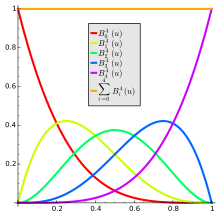
\includegraphics[height=1.5in]{figures/background/Bernstein_curves.png}
    \end{subfigure}%
    ~ 
    \begin{subfigure}[t]{0.5\textwidth}
        \centering
        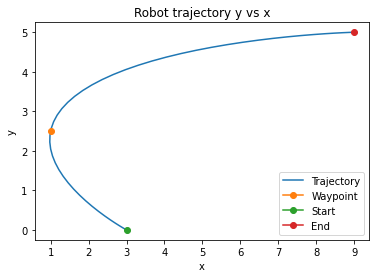
\includegraphics[height=1.5in]{figures/background/holonomic_Bernstein.png}
    \end{subfigure}
    \caption[Bernstein curves and trajectory]{(a) Bernstein basis curves of order-4, (b) An example of a holonomic robot trajectory fitted using order-4 Bernstein polynomials.}
    \label{fig:Bernstein_curv}
\end{figure*}

The trajectory represented as a Bernstein polynomial can be depicted in terms of the basis polynomials and Bernstein coefficients $W_i$ as follows:

\begin{equation}
    f(t) = \sum_{i=0}^{n}W_i \boldsymbol{B_{i,n}(t)}
    \label{eqn:Bernstein}
\end{equation}

The derivatives of the Bernstein basis function are, in themselves, Bernstein polynomials\cite{bernstein_gen}. Similar to eqn. \ref{eqn:cubic_spline}, we can equate the function $f$ at discrete timestamps to obtain the Bernstein coefficients $W_i$ by solving a system of linear equations.

\subsection{Discrete-time representation}

A discrete-time trajectory represented as a sequence of states $f(t) = \{f(t_0), f(t_1), ... f(t_f)\}$ corresponding to successive timestamps $t = \{t_0, t_1, ... t_f\}$. It can be thought of as sampling a continuous-time trajectory function at predefined timestamps. For the purpose of computational representation of trajectories, discrete-time sequences are generally used. To represent a trajectory in continuous time, generally, the basis functions are predetermined and only the coefficients are saved to reconstruct the trajectory as a weighted linear combination of known basis functions, similar to eqns. \ref{eqn:cubic_spline} and \ref{eqn:Bernstein}.


\section{The Trajectory Optimization Problem}
\label{sec:optimization-intro}
\textbf{Linear Programming:}
Solving polynomial coefficients for the boundary state constraints as discussed in section \ref{sec:trajectory_rep} falls into a class of mathematical optimization known as Linear Programming(LP), which, simply put, involves solving a system of linear equations. Eqn. \ref{eqn:LP} with the polynomial weight vector as $W$, the basis polynomial matrix as $B$ and the right-hand side boundary vector $A$ can be solved using LP as follows:
\begin{equation}
    W = inv({B})A
\end{equation}

In addition to solving for boundary constraints, we can define a general objective function($\zeta$) in terms of the trajectory function $f$ that should be subject to the robot's kinematic, dynamic, and environmental equality and inequality constraints $g$. The evaluation of this objective function comes from the motion planning module of the robot system. Mathematically, this optimization problem may be written as:

\begin{equation}
\min_{f(t)} \zeta(f(t)) \qquad \text{st: } g(f(t)) \leq 0
\end{equation}


\textbf{Quadratic Programming:}
For most path planning objectives such as goal-reaching, jerk minimization, and smooth trajectory generation, the cost function $\zeta$ is quadratic with respect to $f$, giving rise to constrained Quadratic Program(QP) optimization, and can be written as follows:


\begin{equation}
\min_{f} \frac{1}{2}f^{T}\boldsymbol{P}f + q^{T}f \qquad
 \text{st: }  Gf \leq h\label{eqn:QP}
\end{equation}

For example, the objective function could be the Euclidean distance of the current position of a robot from the intended goal position, and the constraint matrices $G$ and $h$ could denote the boundary states and velocity limits for the robot. The solution to the above QP optimization problem presents challenges, including the non-convexity of the objective function and its constraints and discontinuities in the objective function. We will now discuss two approaches to solving QP optimization.

\subsection{Gradient-based Optimization}\label{sec:gradient-optim}
The QP optimization proposed in eqn. \ref{eqn:QP} for $\zeta(f) = \frac{1}{2}f^TPf + q^Tf$ can be solved by finding the inflection point in the convex objective curve. To do this, we compute the gradient of the objective function with respect to the optimization variables as follows:


\begin{equation}
    \triangledown_{f}{\zeta} = f^TP + q^T = 0
    \label{eqn:gradient}
\end{equation}

Now, we attempt to attain the minima by updating the optimization variable with an iterative Gradient Descent approach. The update rule for $f$ in the $k^{th}$ optimization iteration for a learning rate of $\alpha > 0$ is as shown below:

\begin{equation}
    f_{k+1}^T = f_k^T - \alpha \triangledown_{f}{\zeta}
\end{equation}

The feasibility of solving the optimization problem with this approach is dependent on factors such as the convexity of the objective function, the convexity of the constraints, and the computational complexity of computing the gradient. A few existing approaches for mobile robot path planning that use gradient-based optimization include \cite{aks_ral21}, and \cite{CDC_time_scaling}. Even for manipulator planning, \cite{CHOMP}, \cite{STOMP} use gradient-based optimization where the gradient of the objective is computed over the joint angle space. 

\subsection{Sampling-based Optimization}\label{sec:sampling-optim}

Sampling-based approaches bypass the gradient computation in eqn.\ref{eqn:gradient} by sampling points in the solution space and picking the sample that minimizes the optimization objective $\zeta$. This approach is adopted in Rapidly-Exploring Random Trees(RRT) \cite{RRT-og}, where around each current point, random uniform samples of points are considered and connected to an expanding tree toward the goal. Similarly, in A* \cite{A*}, Djikstra, and EBS-A* \cite{EBS-A*} algorithms, a heuristic function is optimized over an expanding graph search to compute the most optimal path from a start pose to an end pose. 

Recent approaches \cite{STORM}, \cite{iCEM}, and \cite{VPSTO} sample candidate solutions to the optimization problem from a distribution and compute the cost associated with each candidate. Then the sample distribution is adapted to produce a "better" sample in the next iterations. This translates a deterministic optimization problem into a stochastic optimization problem. The benefit of this approach is its speed and generalizability to non-convex, discontinuous objective functions that would be infeasible to solve using gradient-based optimization techniques. 

\subsection{Collision Avoidance methods}

Collision avoidance for a robot involves the interaction of the robot with its environment and ensuring the following:

\begin{enumerate}
    \item Collision avoidance with static obstacles (e.g, tree on a road, brick wall, etc.)
    \item Collision avoidance with dynamic obstacles (e.g, other moving robots, pedestrians (for cars), birds (for drones) etc.)
    \item \label{point:self-collision}Self-collision avoidance in case of an extended robot, such as a manipulator, between its own links and joints.
\end{enumerate}

Collision detection is usually performed by sensors onboard the robot in simulation or hardware, but for the purpose of path planning, we mathematically estimate collisions using geometric approximations of obstacles and the robot. We assume the map of the environment is known to the robot from the Localization and Mapping modules. Most existing research, such as \cite{RVO}, approximate obstacles of varied shapes by their circumscribing spheres in 3-D or circles in 2-D. The robot itself is reduced to a point object, while its circumscribing radius is added as padding to the obstacles in the environment to account for grazing scenarios to simplify the path-planning process and collision detection. \cite{aks_ral21} estimates obstacles with axis-aligned ellipsoids with padding to generalize to a wider range of obstacles with non-uniform dimensions. 

\subsubsection{Distance-based Collision Avoidance}\label{sec:distance-based-collision}

\textbf{For Mobile Robots:}
For a 2-D mobile robot centered at $(x_r, y_r)$, let us consider a circumscribing circle of radius $R_{bot}$. We aim to avoid collision with an obstacle centered at $(x_o, y_o)$ of a circumscribing radius of $R_{obs}$. To avoid collision of the robot with the obstacle, we need to ensure the Euclidean distance between their centers is greater than or equal to the sum of their radii (the equality holding in the situation where the robot just grazes along the obstacle). Mathematically this can be represented as follows:

\begin{equation}
    \sqrt{(x_r - x_o)^2 + (y_r - y_o)^2} \geq R_{obs}+R_{bot}
\end{equation}

For unequal robot dimensions along the axes, we can estimate the robots with their circumscribing ellipsoids instead of spheres in 3-D. Fig \ref{fig:robot-ellipsoidals} depicts the axis-aligned ellipsoidal robot representation and the distance between them that we use in Chapter \ref{ch:gpu_mat} for our multi-agent optimizer.

\begin{figure}[ht]
    \centering
    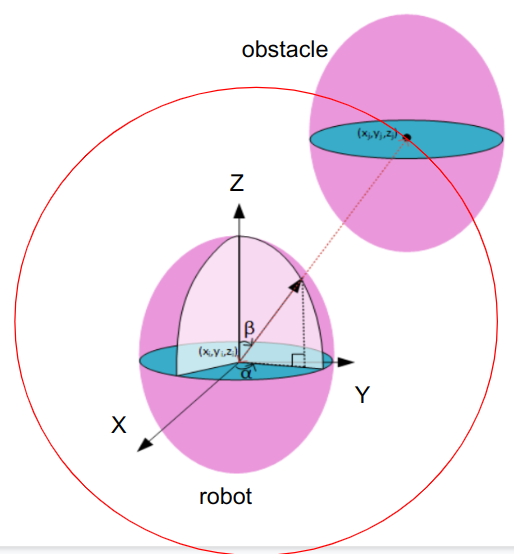
\includegraphics[scale=0.5]{figures/background/ellipsoidals.png}
    \caption[Ellipsoidal Robots]{Axis-aligned ellipses representing robots for collision avoidance in chapter \ref{ch:gpu_mat}.}
    \label{fig:robot-ellipsoidals}
\end{figure}

\textbf{For Manipulators:}
The same approach can be extended to robots moving in higher dimensional spaces. For complex robot systems such as manipulators, distance-based collision avoidance involves self-collision among the robot links, as discussed in point \ref{point:self-collision}, along with collision avoidance with the environment. Based on our literature survey, there are broadly three approaches to solving this problem:
\begin{enumerate}
    \item \label{point: SDF} \textit{Distance of sampled points:} \cite{STOMP} approximates the robot body $B$ as a set of overlapping spheres $b \in B$ of radius $r_l$. We require all points in each sphere to be a distance, at least $\epsilon$ away from the closest obstacle. This constraint can be simplified as the center of the sphere being at least $\epsilon + r_l$ away from obstacles. Thus, our obstacle cost function is as follows:
    \begin{equation}
        q_o(\theta_t) = \sum_{b \in B}{max(\epsilon+r_l - d(x_b),0)||\dot{x_b}||}
    \end{equation}
    
    \item \textit{Implicit Representation Learning-based Collision Avoidance:} \cite{STORM} uses \textit{jointNERF}, a query-able neural network that learns implicit representations of the objects in the environment, including robot links and obstacles, and computes distances between them to detect collisions. 
    
 
\end{enumerate}

This dissertation addresses collisions for manipulators by involving mesh overlaps for collision avoidance in manipulators using the PyBullet simulator. 

\subsubsection{Time-scaling}

A change in the independent variable from $t$ to $\tau$ in the trajectory definition $f(t)$ does not change the path taken by the robot, but brings the following changes in the velocity profile of the trajectory:

\begin{equation}
    \dot{f(\tau)} = \dot{f(t)}\frac{dt}{d\tau}
\end{equation}

The trajectory $f(\tau)$ can be thought of as the robot passing through the same points as $f(t)$, with a scaled version of the original velocity $\dot{f(t)}$, i.e. changing the velocity and acceleration of the robot while keeping its position undisturbed. This transformation in the time scale allows us to regulate the velocity of the robot, playing a key role in collision avoidance. The robot sticks to its original planned global path with a scaled version of its original velocity, and regains its original velocity once the collision with a dynamic obstacle has been avoided. This approach proves to be agnostic to the kinematics of the robot itself since it does not hold any assumptions about the initial trajectory of the robot.

As for the transformation between $t$ and $\tau$, \cite{CDC_time_scaling} experiments with constant as well as exponential time-scaling, estimating the parameters of the transformation function and using them for collision avoidance against workspaces cluttered with dynamic obstacles.

\subsection{Performance Metrics}\label{sec:traj_eval_metrics}

This subsection discusses a few performance metrics that are used to evaluate trajectories obtained from different planning methods. We use the following metrics for bench-marking one algorithm against another:

\begin{itemize}
\item \textit{Smoothness cost:} It is computed as the norm of the second-order finite-difference of the robot position at different time instances. We aim to minimize this smoothness cost to get smooth trajectories feasible for execution through a controller. 
\item \textit{Arc-length:} It is computed as the norm of the first-order finite-difference of the robot positions at different time instances. We aim to minimize arc-length for computed trajectories to ensure short trajectory curves are returned.
\item \textit{Computation Time:} The time taken for each approach to return a smooth and collision-free solution. Depending on the application, we may want computation time in the order of milliseconds for real-time online adaptive planning or in the order of a few seconds for offline planning. 
\item \textit{Success Rate:} It is computed as the number of successful completion of the intended task (such as, reaching a goal, picking up a payload) as a fraction of the total number of tries. An algorithm with a higher success rate will be preferred for the task at hand.
\item \textit{Number of Collisions:} It is calculated as the number of times the robot collides with static and dynamic obstacles, as well as with itself while following a planned trajectory. Lower the number of collisions, the more effective our planning method.
\end{itemize}

\section{Multi-Robot Path Planning}

This section provides a brief overview of the multi-robot path planning problem, including a primer for some of the ideas that shape our algorithm discussed in Chapter \ref{ch:gpu_mat}. 

\subsection{Applications}

Multi-robot systems consist of several interaction-aware robots, each capable of independent decision-making to execute a collective task. The inspiration behind such systems is derived from swarms of bees and other insects. Typical examples of such systems used widely include swarm drones and robot fleets. Multi-robot systems involve coordination and communication among constituent robots, allowing a division of labor to achieve a given task. For example, robot fleets are being extensively used today to perform search-and-rescue missions in areas unsuitable for human intervention, particularly during natural disasters. Swarm drones are also used for imaging and mapping vast territories, particularly for military applications to detect enemy advances. They are also used for demonstrating geometric formations, as well as for military combat, last-mile parcel delivery, and precision agriculture. 

\begin{figure}[ht]
    \centering
    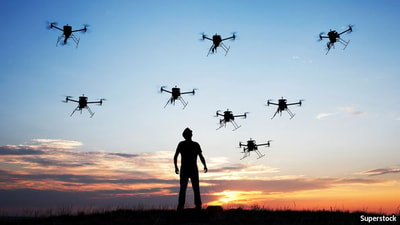
\includegraphics[scale=0.5]{figures/background/swarm_drones.jpg}
    \caption[Swarm Drones]{Swarm drones are used for a wide variety of robotics applications, ranging from search-and-rescue missions, military combat, parcel delivery, and precision agriculture. Source: \scriptsize{\url{https://www.economist.com/the-economist-explains/2015/10/02/how-swarm-drones-are-mimicking-nature}}}
    \label{fig:swarm-drones}
\end{figure}

\subsection{Challenges Involved}\label{sec: multiagent_challenges}

A multi-robot system must ensure that individual robots do not crash into their surroundings or each other. The individual robots must also follow short and safe trajectories from start to goal, and replan their trajectories in near real-time if required. A few challenges associated with multi-robot path planning are as follows:

\begin{enumerate}
    \item \label{bg: centralized_multi_planning}\textit{Coordination and Communication Issues:} Individual robots may communicate directly with each other or relay through a central ground station to share information and coordinate their actions. However, communication and bandwidth limitations can cause delays and disruptions in data transmission. 

    \item \label{bg: scalability_multi_planning}\textit{Scalability Issues:} Multi-robot systems need to perceive their environment accurately to avoid collisions and perform their tasks effectively. However, the limited sensing capabilities of robots and the complexity of the environment can make it difficult to obtain reliable information about the surroundings. Moreover, as the number of drones in a swarm increases, the overhead for collision avoidance also increases since collision constraints need to be computed pairwise.
    
\end{enumerate}

Overall, multi-robot planning and coordination are complex and challenging tasks that require careful consideration of communication, sensing, control, and optimization. Despite these challenges, the potential benefits of swarm drones make them an attractive area of research and development for many applications. To solve problem \ref{bg: centralized_multi_planning}, multi-robot systems typically use decentralized control, meaning that each robot makes decisions for itself without central coordination. We have already discussed Centralized versus Distributed trajectory optimization paradigms in Section \ref{centralized_vs_distributed}, which can solve the scalability issues in problem \ref{bg: scalability_multi_planning}, rising from an increasing number of robots in a multi-robot system. However, the accuracy of distributed multi-robot planning depends on the accuracy of the predictive model each robot uses for the other robots. The algorithms we discuss in the following subsections can be implemented either in a centralized or a distributed setting, depending on the speed, scale and collision avoidance requirements. 

\subsection{Graph-Search-based Multi-Agent Path Finding}\label{sec:MAPF}

Multi-Agent Path Finding(MAPF) consists of a class of algorithms under the umbrella of multi-robot planning that involves the computation of collision-free paths from the start to the goal in a shared environment. Typical solutions for the multi-agent path-finding problem derive inspiration from shortest path computation in graph theory by discretizing the action space of the robots into graph nodes and constructing edges between them based on permissible controls. Let us now discuss some of the different graph-search-based algorithms that have been developed for MAPF:

\subsubsection{A* Algorithm:}\label{sec:A*}
A*\cite{A*} is a popular heuristic search algorithm that can be used for MAPF. It uses an admissible heuristic function to estimate the cost of reaching the goal state, typically based on the distance between agents and their targets. A* algorithm can find optimal solutions but can be slow for large-scale MAPF problems.

\subsubsection{Conflict-based Search(CBS) Algorithm:}
CBS\cite{CBS} is a popular algorithm for solving MAPF problems. CBS is a two-level search algorithm that first searches for individual agent paths and then resolves conflicts between them. CBS can handle a large number of agents and can find optimal solutions for MAPF problems.


\subsubsection{Push and Swap (PaS):}
PaS\cite{PaS} is a local search algorithm that operates by pushing agents and swapping their positions to find a collision-free solution. PaS algorithm is efficient for small-scale MAPF problems but can struggle to find optimal solutions for large-scale problems.

\subsection{Batch Trajectory Optimization}

Batch trajectory optimization can be applied to multi-robot systems, where a group of robots works together to perform a task. In this context, the goal is to optimize the trajectories of all robots in the system to achieve the desired task while minimizing the overall cost of the system. Instead of considering all the robots in the system at once, they could be split into groups or batches that solve the trajectory optimization problem independent of one another as well. A set of candidate trajectories are chosen for each robot based on the robot dynamics and task definition and are optimized for all the robots in a single shot by minimizing the overall cost function for all the robots in the system. The cost function could the the norm of the acceleration of all the robots to ensure precise, smooth movements, or the total time taken by all the robots to execute the given task. Note that this optimization problem also includes collision avoidance constraints between pairs of agents and obstacles in the environment. Then the optimal set of trajectories are executed by all the robots. 

\subsection{Accelerating Batch Optimization over GPUs}

Matrix computations can be sped up over a GPU (Graphics Processing Unit) by taking advantage of the massively parallel architecture of the GPU. A GPU typically contains thousands of small processing cores that work together to perform computations in parallel. Matrix computations, such as matrix multiplication, are particularly well-suited for parallel processing because each element of the output matrix can be computed independently.

To speed up matrix computations on a GPU, the matrix data is first transferred from the CPU memory to the GPU memory. This transfer can be done using specialized libraries such as CUDA, which is a parallel computing platform and programming model developed by NVIDIA for general-purpose computing on GPUs. Once the matrix data is in the GPU memory, the computation is split into many smaller computations that can be performed in parallel across the thousands of cores on the GPU. For example, in matrix multiplication, each output element can be computed by multiplying the corresponding row of the first matrix by the corresponding column of the second matrix. By breaking the computation down into smaller tasks that can be performed in parallel, the GPU can perform matrix computations much faster than a CPU, which typically has fewer processing cores.

We use the JAX library \cite{bradbury2020jax}, developed by Google in Chapter \ref{ch:gpu_mat} to accelerate matrix operations. Additional details and usage of the JAX NumPy library has been discussed in Appendix \ref{appendix:JAX}



\section{Manipulator Path Planning}

This section provides a brief overview of the kinematics of robot manipulators and introduces the task of path planning for manipulators, as a background for our approach discussed in Chapter \ref{ch:bl_arm}.

The problem of robot manipulator path planning is the task of finding a collision-free path for a robotic arm to move from its initial position to a desired final position while avoiding obstacles in its workspace. This is a challenging problem because the workspace of the robot can be complex and high-dimensional, and the motion of the robot can be constrained by its physical limits, such as joint velocity and angle limits. Path planning algorithms must take into account these constraints and find an optimal path that satisfies the constraints while minimizing some performance criteria, such as the path length or the time required to complete the motion. This problem is relevant in many applications of robotics, including industrial automation, manufacturing, and healthcare, where robots are used to perform repetitive or complex tasks in a safe and efficient manner. An example of path planning required for a robot manipulator is illustrated in Figure \ref{fig:manipulator-planning}.

\begin{figure}[ht]
    \centering
    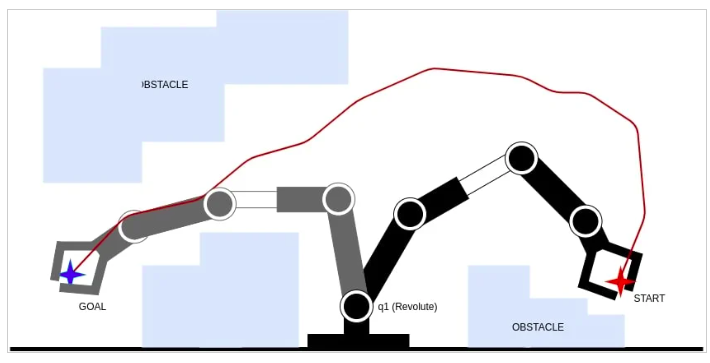
\includegraphics[scale=0.5]{figures/background/manipulator_planning.png}
    \caption[Path Planning for a Manipulator]{An illustration showing the task of path planning for a robot manipulator from a start pose to an end pose, while avoiding obstacles in the surroundings and preventing self-collisions and coiling in on itself. The red line denotes the trajectory to be followed by the end-effector from start to goal. Source: \scriptsize{\url{https://control.com/technical-articles/how-does-motion-planning-for-autonomous-robot-manipulation-work/}}}
    \label{fig:manipulator-planning}
\end{figure}


\subsection{Manipulator Kinematics}\label{sec:bg-manipulator-kinematics}

In the context of this thesis, we discuss the manipulator planning problem primarily for two robot manipulators - Franka Emika Panda robot arm and Universal Robots(UR5e) robot arm. The number of degrees of freedom(DoF) for the former is 7, while that for the latter is 6. Figure \ref{fig:Franka-Panda} shows the Franka Panda robot manipulator against its links and joints, while Figure \ref{fig:ur5e} denotes the same for the UR5e robot arm. 

\begin{figure*}[t!]
    \centering
    \begin{subfigure}[t]{0.4\textwidth}
        \centering
        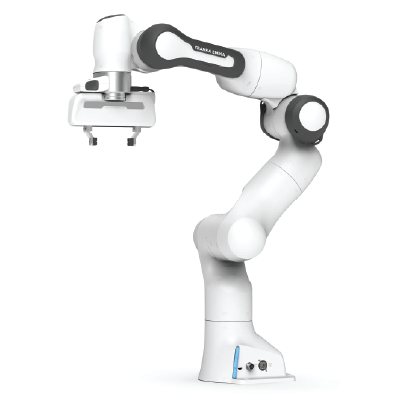
\includegraphics[height=1.5in]{figures/background/franka_overview.png}
    \end{subfigure}%
    ~ 
    \begin{subfigure}[t]{0.5\textwidth}
        \centering
        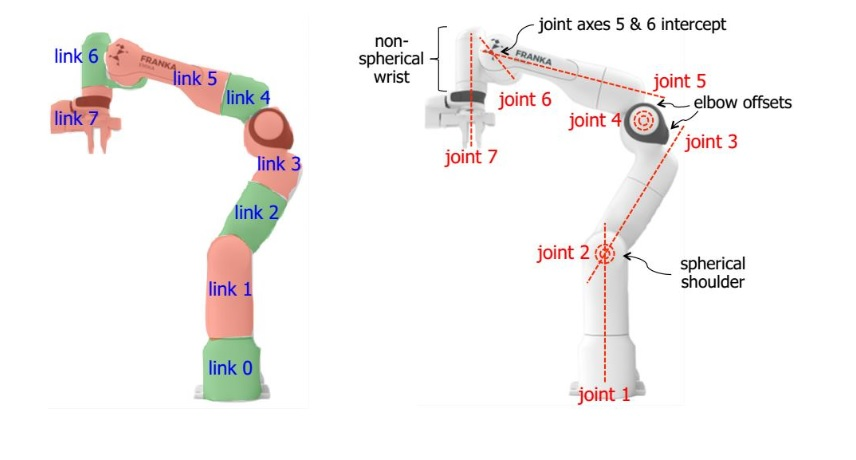
\includegraphics[height=1.5in]{figures/background/franka_links.png}
    \end{subfigure}
    \caption[Franka Emika Panda Robot Arm]{(a) The Franka Emika Panda Robot Arm with an end-effector(two-finger gripper)(b) The links and types of joints and their locations for the 7-DoF Franka Panda manipulator.}
    \label{fig:Franka-Panda}
\end{figure*}

The kinematics of a robot manipulator describes the relationship between the joint angles and the position and orientation of the end-effector of the robot. Forward kinematics denotes the transformation of joint angles to an end-effector position, while inverse kinematics attempts to calculate the required joint angles to achieve a desired end-effector position. We will now discuss the forward kinematics of both manipulators mathematically.

\subsubsection{Franka Emika Panda}

The Franka Emika Panda is a 7 degree-of-freedom robot manipulator that is widely used in research and industrial applications. The Panda robot has a serial kinematic structure, where each joint is connected to the previous joint and to the base of the robot. The joint angles, corresponding to the 7 joints, shown in Figure \ref{fig:Franka-Panda} are denoted by $q_1$, $q_2$, ..., $q_7$, corresponding to the rotations of each joint around its respective axis. The position and orientation of the end-effector are represented by a $4$x$4$ transformation matrix $T$. The forward kinematics of the Panda robot can be described by the following equations:

\begin{equation}
    T = T_1T_2T_3T_4T_5T_6T_7
    \label{eqn: fk_manipulator}
\end{equation}


where $T_i$ is the transformation matrix corresponding to the $i^{th}$ joint of the robot. These transformation matrices can be computed from the Denavit-Hartenberg parameters, which describe the geometry and kinematics of the robot as per the following equation:

\begin{equation}
    T_i = \begin{bmatrix}
    \cos(\theta_i) & -\sin(\theta_i)\cos(\alpha_i) & \sin(\theta_i)\sin(\alpha_i) & a_i\cos(\theta_i)\\
    \sin(\theta_i) & \cos(\theta_i)\cos(\alpha_i) & 
    -\cos(\theta_i)\sin(\alpha_i) & a_i\sin(\theta_i)\\
    0 & \sin(\alpha_i) & \cos(\alpha_i) & d_i \\
    0 & 0 & 0 & 1
    \end{bmatrix}
\end{equation}



The Denavit-Hartenberg frames and parameters for the Franka Panda robot arm are depicted in Figure \ref{fig:dh-franka}.

\begin{figure}[ht]
    \centering
    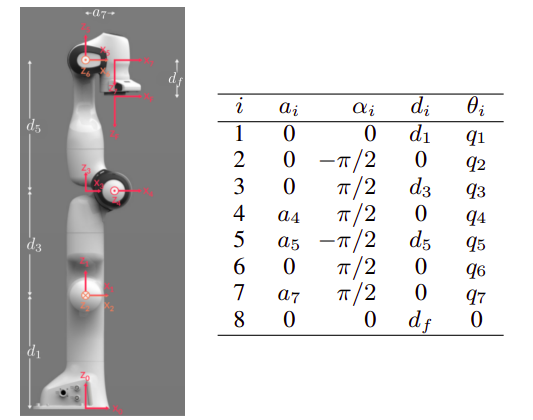
\includegraphics[scale=0.5]{figures/background/dh-franka.png}
    \caption[DH Parameters for the Franka Panda Arm]{Denavit-Hartenberg(D-H) frames and parameters for the 7-DoF Franka Panda robot arm. Source: \cite{DH-Franka}.}
    \label{fig:dh-franka}
\end{figure}

\subsubsection{UR5e}

\begin{figure*}[t!]
    \centering
    \begin{subfigure}[t]{0.4\textwidth}
        \centering
        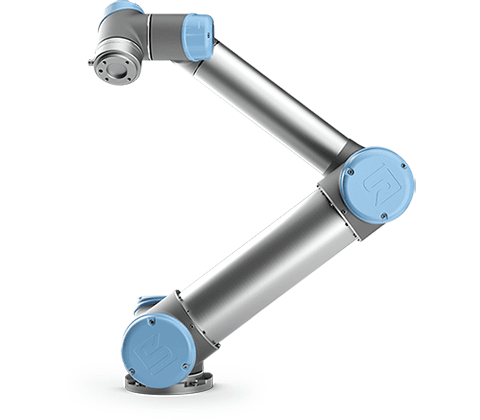
\includegraphics[height=1.5in]{figures/background/ur5e_overview.png}
    \end{subfigure}%
    ~ 
    \begin{subfigure}[t]{0.5\textwidth}
        \centering
        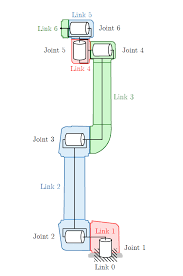
\includegraphics[height=1.5in]{figures/background/ur5e_links.png}
    \end{subfigure}
    \caption[Universal Robots(UR5e) Robot Arm]{(a) The Universal Robots(UR5e) Robot Arm (b) The links and types of joints and their locations for the 6-DoF UR5e manipulator.}
    \label{fig:ur5e}
\end{figure*}

The Universal Robots UR5e is a 6-degree-of-freedom robot arm. The joint angles, corresponding to the 6 joints, shown in Figure \ref{fig:ur5e} are denoted by $q_1$, $q_2$, ..., $q_6$, and the overall forward kinematics is described by the serial multiplication of six transformation matrices corresponding to the six joints, similar to eqn.\ref{eqn: fk_manipulator}. The Denavit-Hartenberg(D-H) frames and parameters for the 6-DoF UR5e robot arm are depicted in Figure \ref{fig:dh-ur5}.

\begin{figure*}[t!]
    \centering
    \begin{subfigure}[t]{0.5\textwidth}
        \centering
        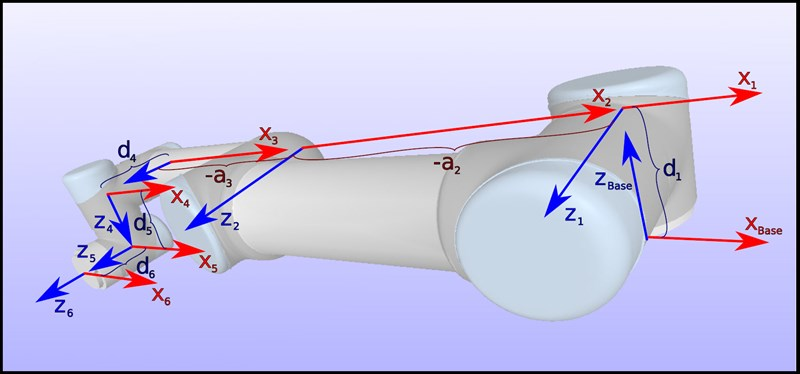
\includegraphics[height=1.5in]{figures/background/dh_ur5ea.jpg}
    \end{subfigure}%
    ~ 
    \begin{subfigure}[t]{0.3\textwidth}
        \centering
        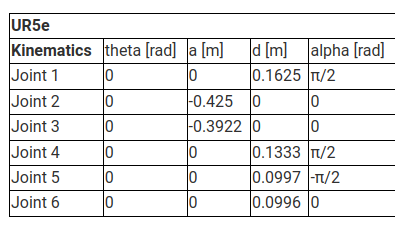
\includegraphics[height=1.5in]{figures/background/dh_ur5eb.png}
    \end{subfigure}
    \caption[DH Parameters for the UR5e Arm]{Denavit-Hartenberg(D-H) frames and parameters for the 6-DoF UR5e robot arm. Source: \scriptsize{\url{https://www.universal-robots.com/articles/ur/application-installation/dh-parameters-for-calculations-of-kinematics-and-dynamics}}}
    \label{fig:dh-ur5}
\end{figure*}

\subsection{Challenges Involved}

Path planning for robot manipulators is a complex problem that involves several challenges. Here are some of the key challenges involved:

\begin{itemize}
    \item \textit{High Dimensionality:} Robot manipulators typically operate in high-dimensional spaces, with each joint providing a degree of freedom, such as the 7-dimensional joint angle space in the case of the Franka Panda arm and the 6-dimensional joint space for the UR5e arm. This makes the search space for path-planning algorithms very large, and finding an optimal path becomes computationally expensive.
    \item \textit{Nonlinear Constraints:}  The motion of robot manipulators is subject to nonlinear constraints, such as the dynamics of the robot and the workspace bounds, as well as physical constraints, such as joint limits and collision avoidance. Incorporating these constraints into path-planning algorithms can be challenging, and some algorithms may require sophisticated mathematical techniques to solve the constraints.
    \item \textit{Real-time Operation:}  In many rearrangement applications, path planning must be performed in real-time, with the manipulator making decisions and adapting to new obstacles or changes in the environment. Real-time path planning requires efficient algorithms that can quickly search the space of possible paths and adapt the plan as needed.
\end{itemize}

Overcoming the above challenges requires the development of efficient path-planning algorithms that can handle these constraints and produce high-quality paths. We attempt to address all these challenges through our bi-level trajectory optimizer for manipulators discussed in Chapter \ref{ch:bl_arm}.

\subsection{Joint space-vs end-effector space}

For a robot manipulator, the path-planning can be performed in two motion spaces - either in the high-dimensional space formed by the joint angles corresponding to each movable joint or the end-effector space, which is a 3-dimensional space limited by the workspace bounds  or a 2-dimensional table plane (for planar end-effector motion). The choice of motion space is determined by the requirements of the task at hand. For example, for a robot arm pushing objects on the table, the major task at hand involves the pose of the end-effector on the 2-D tabletop plane, and hence the path planning can be performed in the Cartesian end-effector space or even in the Cartesian space of the center of the object being pushed on the table. For tasks involving grasping objects, it is more effective to plan trajectories in the joint space in order to avoid collisions and minimize joint movements. 

Based on the two paradigms of optimization discussed in Sections \ref{sec:gradient-optim} and \ref{sec:sampling-optim}, let us discuss both Gradient-based and Sampling-based trajectory optimization for a robot manipulator.

\subsection{Gradient-based Optimization}\label{sec:bg-gradient-manipulator}

\subsubsection{CHOMP}\label{sec:CHOMP}

CHOMP (Covariant Hamiltonian Optimization for Motion Planning)\cite{CHOMP} is a gradient-based optimization method for efficient motion planning of robot manipulators in high-dimensional spaces. This method was developed by Brian Paden and Emo Todorov in 2011.

The key idea behind CHOMP is to formulate the motion planning problem as an optimization problem, where the objective is to minimize an objective function that typically includes terms that penalize collisions with obstacles, deviation from a desired trajectory, and energy consumption. In CHOMP, the optimization is performed using a gradient descent method, where the gradient of the cost function with respect to the joint angles of the robot is computed and used to update the joint angles iteratively. The gradient is computed using backpropagation through time, which involves propagating the gradient backward through a sequence of time steps.

One of the key advantages of CHOMP is its ability to handle non-convex constraints and to generate smooth, continuous paths that avoid collisions with obstacles. This is achieved by using a smoothing term in the cost function, which encourages the joint angles to vary smoothly over time. Another advantage of CHOMP is its scalability to high-dimensional spaces, which makes it well-suited for motion planning of robot manipulators with many degrees of freedom.

However, CHOMP does have some limitations. It requires a good initial guess of the path, which can be challenging in complex environments with many obstacles. The optimization can also converge to local minima, which can result in suboptimal paths. Further, CHOMP involves gradient computations which may get intractable to compute in very high-dimensional spaces and spend a significant amount of time to return a feasible trajectory, eliminating the scope of real-time path planning. To address these limitations, various extensions and modifications to CHOMP have been proposed, such as incorporating stochastic optimization or combining CHOMP with other planning algorithms.


\subsubsection{TrajOpt}\label{sec:TrajOpt}

TrajOpt\cite{TrajOpt}, developed by John Schulman and his colleagues at UC Berkeley in 2013, is an open-source library for motion planning and trajectory optimization of robot manipulators.

TrajOpt also involves gradient-based trajectory optimization using techniques such as sequential quadratic programming or gradient descent. The TrajOpt library provides a flexible and modular framework for specifying the motion planning problem, allowing users to define a wide range of cost functions and constraints, including collision avoidance, joint limits, end-effector constraints, and task-specific objectives such as minimizing energy consumption. TrajOpt also uses a collision-checking algorithm based on bounding volume hierarchies, which can quickly identify potential collisions between the robot and the environment. It also incorporates a warm-starting strategy, which initializes the optimization algorithm with a feasible solution from a previous iteration, reducing the time required for convergence.

TrajOpt, written in C++ and Python, is designed to be highly customizable and extensible. It can be integrated with various robot simulation and control frameworks, such as ROS, Gazebo, or PyBullet, and supports a wide range of environments, robot models, and kinematic solvers. \cite{OpenRAVE} uses TrajOpt as a collision-detection module.

\subsection{Sampling-based Optimization}\label{sec:bg-sampling-manipulator}

Sampling-based optimizers rely on stochastic optimization, i.e. sampling a set of potential candidate trajectories to be followed by the manipulator and evaluating the associated costs to finally choose the trajectory with the minimum cost. The best set of candidates is used to iteratively improve on the samples for the next iteration, ultimately helping the optimizer converge to an optimum in the cost function. 

\subsubsection{STORM}

STORM(Stochastic Tensor Optimization for Robot Motion)\cite{STORM} is an optimization algorithm designed to efficiently and effectively generate smooth and collision-free trajectories for robots in complex environments between a start state and a desired state by iteratively optimizing a tensor-based cost function. STORM works by first defining a tensor-based representation of the state space, designed to capture the high-dimensional motion space of the robot. The tensor is defined as a multi-dimensional array, where each dimension corresponds to a specific aspect of the robot's state, such as position, velocity, or acceleration. The size of each dimension is determined by the resolution of the state space.

The optimization process is stochastic, which means that it involves randomly sampling different trajectories and evaluating their costs. Self-collisions are detected by using \textit{jointNERF}, a network that computes the closest distance between robot links given joint poses, while environment collisions are based on signed distances. This randomness helps to ensure that STORM is able to find a diverse set of trajectories that can be used to navigate complex environments. Additionally, STORM is able to leverage parallel computing to speed up the optimization process, which can be critical for real-time applications.

One of the key advantages of STORM is its ability to handle high-dimensional state spaces, which is particularly useful for manipulator path planning. It achieves this by using a tensor-based representation of the state space, which allows it to efficiently explore large and complex environments. STORM is also able to incorporate a wide range of constraints, including collision avoidance, joint limits, and kinematic constraints.

\subsubsection{Cross-Entropy Methods(CEM)}

The cross-entropy method (CEM)\cite{CEM_og} is a derivative-free optimization technique that employs an adaptive importance sampling procedure using the cross-entropy measure. In each iteration of the CEM-based stochastic trajectory optimization, the following two steps are performed:

\begin{itemize}
    \item Derive candidate trajectories by sampling from a probability distribution
    \item Minimize the cross-entropy between the sample distribution and a target distribution to update the parameters of the former.
\end{itemize}

Mathematically, these steps can be represented as follows (Source: \url{https://en.wikipedia.org/wiki/Cross-entropy_method}):

\begin{enumerate}
    \item Choose initial parameter vector $\boldsymbol{v}^{0}$; set t = 1
    \item \label{point:sampling}Generate a random sample $\boldsymbol{X_1}$, ...,$\boldsymbol{X_N}$ from $f(\boldsymbol{v^{(t-1)}})$.
    \item Solve for $\boldsymbol{v^{(t)}}$, for a given cost function $\zeta$ where,
    \begin{equation}
        \boldsymbol{v^{(t)}} = \argmax_v\frac{1}{N}\sum_{i=1}^{N}\zeta(\boldsymbol{X_i})\frac{f(\boldsymbol{X_i};u)}{f(\boldsymbol{X_i},\boldsymbol{v^{(t-1)}})}\text{log}f(\boldsymbol{X_i};\boldsymbol{v})
    \end{equation}
    \item If convergence is reached, then stop, otherwise proceed to the next iteration by incrementing $t$ by 1 and repeat from step \ref{point:sampling}.
\end{enumerate}

The cost function $\zeta$ takes into account factors such as the length of the path, the amount of time it takes to complete the path, and the distance from the robot arm to obstacles in the environment. Over time, the CEM algorithm converges to an optimal solution, which represents the best path for the robot arm to reach the target point while avoiding obstacles. 

We use an improved version of CEM, called Via-Point Stochastic Trajectory Optimization(VP-STO)\cite{VP-STO} for manipulator path planning in Chapter \ref{ch:bl_arm}.

%--------------------------------------------------------

\chapter{Fast Joint Multi-Robot Trajectory Optimization by GPU Accelerated Batch Solution of Distributed Sub-Problems}
\label{ch:gpu_mat}

\noindent In this chapter, we design a novel approach to solve our research problem \textbf{T2} from Section \ref{intro:multi-robot_aim} - a joint multi-robot trajectory optimizer that can compute trajectories for tens of robots within a small fraction of a second. The computational efficiency of our approach is built on breaking the per-iteration computation of the joint optimization into smaller, decoupled sub-problems and solving them in parallel through a custom batch optimizer. By achieving near real-time planning through a distributed optimization paradigm, we are able to address challenges involving both coordination and scalability in a multi-robot system, discussed in Section \ref{sec: multiagent_challenges}.

{\small \textit{(Published in the journal Frontiers in Robotics and AI, Vol. 9, 2022.  \cite{self-gpu-mat}, also presented at the DMMAS workshop, International Conference on Intelligent Robots and Systems (IROS) 2022.)}}    
%\tableofcontents


\section{Introduction}

Deployment of multiple aerial vehicles such as quadrotors is critical for applications like search and rescue and exploration and mapping of large areas \citep{schranz2020swarm}. Over the last decade, robot fleets have also become ubiquitous in applications like ware-house automation that have a substantial economic impact on society \citep{bolu2021adaptive,priority_seq}. Furthermore, with the advent of connected autonomous cars, it becomes imperative also to view urban mobility as a multi-robot system \citep{zhou2017collision}. A fundamental component of any multi-robot system is the coordination planning that guides individual robots between their start and goal locations while avoiding collisions with the environment and other robots. In this chapter, we adopt the optimization perspective for multi-robot motion planning \citep{aks_ral21}. In this context, the existing approaches broadly fall into two spectra. On one end, we have the centralized approaches wherein the trajectory of all the robots are computed together. The centralized approach can be further subdivided into sequential \citep{incremental_scp_how}, \cite{park2020efficient} and joint optimization \citep{rafaella_scp}, \citep{aks_ral21} respectively depending on whether the trajectories of the robots are computed one at a time or simultaneously. On the other end of the spectrum, we have online distributed model predictive control (DMPC) \citep{dmpc_carlos}, \citep{dmpc_epfl} based approaches wherein each individual robot computes its trajectories in a decoupled manner based on the trajectory prediction of the other robots in the environment. In some works, the prediction module is replaced by robots communicating their current trajectory with each other \citep{dmpc_carlos_2}. 

Centralized approaches, especially the joint optimization variants, provide a rigorous treatment of the collision avoidance constraints and access a larger feasible space formed by all trajectory variables of all the robots. However, joint optimization quickly becomes intractable as the number of robots increases \citep{chen2015decoupled}. In contrast, the distributed MPC approaches can run in real-time but can lead to oscillatory behaviors, and consequently, low success rates of collision avoidance \citep{dmpc_carlos}, \citep{dmpc_carlos_2}. This is because the trajectories computed at each control cycle by any robot are only collision-free with respect to the predicted (or prior communicated ) trajectories of other robots and not the actual trajectories followed by them. 

Our main motivation in this chapter is to improve the computational tractability of multi-robot trajectory planning using a distributed optimization approach to the extent that it becomes possible to compute trajectories for tens of robots in densely cluttered environments in a few tens of milliseconds. To put in context, the said timing is several orders of magnitude faster than some of the existing approaches for joint multi-robot trajectory optimization \citep{rafaella_scp}, \citep{alonso_mora_nips_multi}. Such improvements in computation time would ensure the applicability of our approach for even online re-planning besides the standard use case of computing offline global trajectories for the robots. For example, consider a scenario wherein each robot uses local real-time planners such as Dynamic Window Approach \citep{dwa} or DMPC \citep{dmpc_carlos} to avoid collisions with other robots in a distributive manner. Our approach could provide global re-planning for the local planners at more 5Hz. or more.

On the application side, our main focus is on coordination of multiple quadrotors, typically for applications like search and rescue and coordinated exploration. These applications require point-to-point, collision-free navigation and forms the main benchmark in our experiments. However, our algorithm can be useful for coordination of multiple wheeled mobile robots and even autonomous cars.


% An improvement in joint multi-robot trajectory optimization will be 






% Furthermore, the trajectories computed from our approach can also be used to warm-start the distributed MPC approaches.



\noindent \textbf{Contributions:}
The computational efficiency of our approach is built on several layers of reformulation of the underlying numerical aspects of the joint multi-robot trajectory optimization. We summarize the key points and the benefits that it leads to below.
 
\noindent \textbf{Algorithmic:} Our main idea is to break the per-iteration computation of the joint multi-robot trajectory optimization into smaller, distributed sub-problems by leveraging the solution computed in the previous iterations. Although similar ideas have appeared in many existing works \citep{alonso_mora_nips_multi}, \citep{dmpc_carlos_2}, a core challenge remains: how to efficiently solve the decoupled problem arising at each iteration in parallel. The basic assumption is that the decoupled optimizations can be parallelized across separate CPU threads \citep{alonso_mora_nips_multi}. However, our recent works have shown that such a parallelization approach does not scale well with an increase in the number of problems \citep{aks_behavior_ral22}. The inherent limitation stems from the available CPU cores and thread synchronization issues. 

Thus our main algorithmic contribution in this chapter lies in deriving a novel optimizer that can be efficiently run in a batch setting. In other words, our optimizer can take a set of decoupled optimization problems and vectorize the underlying numerical computations across multiple problem instances. Consider an optimizer that solves a given problem by adding two vectors as a hypothetical example. We can trivially vectorize the computation over different problem instances by stacking each problem's vectors together in the form of a matrix and adding them together. Moreover, this matrix addition can be easily parallelized over GPUs for many problem instances. Our proposed optimizer achieves similar vectorization but for a set of difficult non-convex sub-problems, resulting in each iteration of joint multi-robot trajectory optimization. Specifically, we show that solving the decoupled sub-problems predominantly reduces to solving novel equality constrained quadratic programming (QP) problems under certain collision constraint reformulations. The novelty of the QPs stems from the fact that they all share the same matrices (e.g., Hessian), and only the vectors associated with the QPs vary across the sub-problems. We show that solving all the QP sub-problems in one shot reduces to computing one large matrix-vector product that can be trivially parallelized over GPUs using off-the-shelf linear algebra solvers.  


\noindent \textbf{Applied:} We release our entire implementation for review and to promote further research on this problem. We also release the benchmark data sets used in our simulations.

\noindent \textbf{State-of-the-art Performance} We compare our GPU accelerated optimizer with two strong baselines  \citep{park2020efficient,aks_ral21} and show massive improvement in computation time while being competitive in trajectory quality as measured by metrics like arc-length and smoothness. Our first comparison is with \citep{park2020efficient} that uses a sequential approach for multi-robot trajectory optimization. Our computation time is at least $76.48\%$ lower than that of \citep{park2020efficient} for a smaller problem size involving $16$ robots. Moreover, the performance gap increases substantially in our favor as we increase the number of robots and make the environment more cluttered by introducing more static obstacles. We observe similar trends in trajectory arc-length and smoothness comparison between the two approaches. Our second comparison is with \citep{aks_ral21} that searches directly in the feasible joint space formed by all the pair-wise collision avoidance constraints. Our proposed optimizer shows improved scalability over \citep{aks_ral21} for a larger number of robots while being also superior in trajectory arc length and smoothness.

\section{Problem Formulation and Related Work}
This section introduces the general problem formulation for multi-robot trajectory optimization. We subsequently use the problem set-up to review existing works and contrast our optimizer with them. We begin by summarizing the main symbols and notations used throughout the chapter.

\subsection{Symbols and Notations}
\noindent In this chapter, the lower normal and bold letters denote the scalars and vectors, respectively, while the upper bold case variants represent matrices. The left and right super-scripts denoted by $k$ and $T$ will be used to denote the iteration index of the optimizer and transpose of the vectors and matrices. The time-stamp of any variable will be denoted by $t$. The symbol $\left\Vert \textbf{.} \right\Vert_{2}$ stands for $l_{2}$ norm. We summarize some of the main symbols in Table \eqref{table_1} while some are also introduced in their first place of use. At some places, we perform a special construction where time-stamped variables are stacked to form a vector. For example, $\textbf{x}_i$ will be formed by stacking $x_i(t)$ at different time instants.


\subsection{Robot Kinematics}
\noindent Our optimizer is designed for robots with holonomic motion models. That is, the motion along each axis is decoupled from each other. This is a common assumption made in quadrotor motion planning. Many commercially available wheeled mobile robots also have similar kinematic model. Under certain conditions, even motion planning for car-like vehicles also adopt similar kinematic model and thus our optimizer is suitable for those as well \cite{frenet_planner}.


\subsection{Trajectory Optimization }
\noindent For holonomic robots modeled as series of integrators, the joint trajectory optimization can be formulated in the following manner.

\begin{subequations}
\begin{align}
\min_{x_{i}(t), y_{i}(t), z_{i}(t)} \sum_{t, i} \Big(\ddot{x}_{i}^2(t)+\ddot{y}_{i}^2(t)+\ddot{z}_{i}^2(t)\Big),\label{cost_multirobot} \\
\Big(x_i(t_0), \dot{x}_i(t_0), \ddot{x}_i(t_0), y_i(t_0), \dot{y}_i(t_0), \ddot{y}_i(t_0), z_i(t_0), \dot{z}_i(t_0), \ddot{z}_i(t_0)) = \textbf{b}_{o, i}, \forall i \label{initial_boundary_cond} \\
\Big(x_i(t_f), \dot{x}_i(t_f), \ddot{x}_i(t_f), y_i(t_f), \dot{y}_i(t_f), \ddot{y}_i(t_f), z_i(t_f), \dot{z}_i(t_f), \ddot{z}_i(t_f)) = \textbf{b}_{f, i}, \forall i \label{final_boundary_cond} \\
  -\left(\begin{matrix}
 x_i(t)-x_j(t)\\
 y_i(t)-y_j(t)\\
 z_i(t)-z_j(t)\\
 \end{matrix}\right)^T\textbf{S}\left(\begin{matrix}
 x_i(t)-x_j(t)\\
 y_i(t)-y_j(t)\\
 z_i(t)-z_j(t)\\
 \end{matrix}\right)+1 \leq 0, \forall t,  \{i,j \in \{1,2,...,n_{r}\}, j \neq  i\} \label{coll_multirobot}, \textbf{S} = \begin{bmatrix}
 a^2 & 0 & 0 \\
 0 & a^2 & 0 \\
 0 & 0 & b^2 \\
 \end{bmatrix}
 \end{align}
\end{subequations}

\noindent The cost function (\ref{cost_multirobot}) minimizes the squared norm of the acceleration at each time instant for all the robots. The equality constraints  \eqref{initial_boundary_cond}-\eqref{final_boundary_cond} enforces the initial and final boundary conditions on positions, velocity, and accelerations on each robot trajectory. The pair-wise collision avoidance constraints are modeled by inequalities (\ref{coll_multirobot}), wherein we have assumed that the robots are shaped as axis-aligned spheroids with axis dimensions $(a, a, b)$. For the ease of exposition, we consider all robots to have the same shape. Extension to a more general setting is trivial. The constraints  (\ref{coll_multirobot})  are typically enforced at pre-selected discrete time-stamps, and thus a fine resolution of discretization is necessary for accurately satisfying the constraints. For now, we do not consider any static obstacles in the environment in the formulation above. The extension is trivial as static obstacles can be considered robots with zero velocity and whose trajectories are not updated within the optimizer's iteration.

Let the trajectory of each robot along each motion axis $x, y, z$ be parameterized through $n_v$ number of variables. For example, these variables could be time-stamped way-points representing the trajectory or the coefficients of their polynomial representation (see \eqref{param}). Then, for a set-up with $n_r$ number of robots and a planning horizon of $n_p$, optimization (\ref{cost_multirobot})-(\ref{coll_multirobot}) involves $n_r*n_v$ variables, and $18*n_r$ equality constraints. The number of pair-wise collision constraints would be ${n_r\choose{2}}*n_p$. 

The number of decision variables in optimization (\ref{cost_multirobot})-(\ref{coll_multirobot}) scales linearly with the number of robots. Although this increase poses a computational challenge, the main difficulty in solving the optimization stems from the non-convex pair-wise collision avoidance constraints (\ref{coll_multirobot}) as the rest of the cost and constraint functions are convex. Moreover, the number of collision avoidance constraints increases exponentially with the number of robots. Existing works  \citep{rafaella_scp,aks_ral21, incremental_scp_how, priority_seq, park2020efficient} have adopted different simplifications on the collision avoidance constraints to make multi-robot trajectory optimization more tractable. We thus next present a categorization of these works based on the exact methodology used.

\subsection{Literature Review}
\subsubsection{Joint Optimization with Conservative Convex Approximation}
\noindent The most conceptually simple approach is to solve (\ref{cost_multirobot})-(\ref{coll_multirobot}) as one large optimization problem, wherein the trajectory of every robot is computed in one shot. Authors in \citep{rafaella_scp} simplified the joint optimization by deriving a conservative affine approximation of the collision avoidance constraints (\ref{coll_multirobot}) and consequently reducing  (\ref{cost_multirobot})-(\ref{coll_multirobot}) to a sequence of QPs. As a result, their solution process becomes somewhat tractable for a moderate number of robots ($\approx 10$). However, the computation time of \citep{rafaella_scp} scales poorly because the number of affine constraints still increases exponentially with the number of robots. Our prior work \citep{aks_ral21} substantially improved the scalability of joint multi-robot trajectory optimization by reformulating the Euclidean collision constraints (\ref{coll_multirobot}) into polar form and augmenting them into the cost function by using concepts from the Alternating Direction Method of Multipliers (ADMM). Moreover, we showed that such reduction allowed one-time offline caching of the most expensive parts of the computation. As a result, \citep{aks_ral21} achieved over two orders of magnitude speed-up over \citep{rafaella_scp} for 16 robots. The current proposed work provides a further significant improvement over \citep{aks_ral21} in computation time and trajectory quality.

\subsubsection{Sequential Optimization}

Sequential planners plan for only one robot at a time. At any given planning cycle, the previously computed robot trajectories are considered dynamic obstacles for the currently planned robot. As a result, these approaches ensure that the number of decision variables does not increase with robots. Moreover, the number of collision avoidance constraints increases linearly as the planning cycle progresses. However, note that the linear increase in the number of constraints does not translate to similar scaling in computation time. Even state-of-the-art interior-point solvers have cubic complexity with respect to the number of constraints.

A critical disadvantage of sequential planners is that each subsequent robot has access to less feasible space to maneuver. As a result, optimization problems become progressively constrained as the planning cycle progresses, leading to potential infeasibility. Authors in \citep{incremental_scp_how} tackle this problem by developing an incremental constraint tightening approach. The authors integrate a subset of collision avoidance constraints into the optimization problem, and the size of this set is gradually increased based on the actual collision residuals.

Sequential planners naturally have the notion of priority, and these can be chosen carefully for improved performance. For example, \citep{priority_seq} adopts a priority-based optimization method in which the robots are divided into groups/batches with pre-determined priorities, and the trajectory optimization problem is solved from the highest to the lowest priority group. Similar approach was adopted in \citep{park2020efficient}. Performing sequential planning over a small batch of robots reduces its conservativeness. On the other hand, it introduces an additional challenge of ensuring collision amongst the robots in a given batch. Authors in \citep{park2020efficient} tackle this bottleneck by leveraging graph-based Multi-robot Path Finding (MAPF) methods.



% and solves the collision avoidance problem with respect to all other dummy robots in each iteration. In the next iteration, the robots in the current batch are used as dummy robots, and the process is sequentially repeated. The collision avoidance constraints are expressed in terms of Bernstein polynomials and the initial trajectory is planned using a graph-based Multi-robot Path Finding (MAPF) method. We benchmark our approach against this algorithm and achieve remarkable improvements in computation time by leveraging GPU computations, while maintaining comparable trajectory quality.


% Priorities are assigned based on the occurrence of robot triplets whose trajectories are coupled due to their closeness to one another.
\subsubsection{Distributed Optimization} 

Distributed optimizers at each iteration, break (\ref{cost_multirobot})-(\ref{coll_multirobot}) into decoupled smaller problems. For example, see \citep{alonso_mora_nips_multi}, \citep{multi_robot_1}. The key insight upon which all existing works build is that the only coupling between different robots stem from the pair-wise collision constraints (\ref{coll_multirobot}) \citep{multi_robot_1}. Thus, we if we discard this coupling, (\ref{cost_multirobot})-(\ref{coll_multirobot}) can be easily reduced to $n_r$ number of decoupled optimizations. One way to achieve the said decoupling is to let each robot make prediction of how the trajectories of other robots are going to look in the immediate next iterations and use that to simplify the collision avoidance constraints. More formally, let $(\overline{x}_j(t), \overline{y}_j(t), \overline{z}_j(t) )$ be the predicted position of $j^{th}$ robot at time $t$. Then, the collision avoidance constraints can be simplified as (\ref{distributed_coll}). 


\begin{figure}
    \centering
    {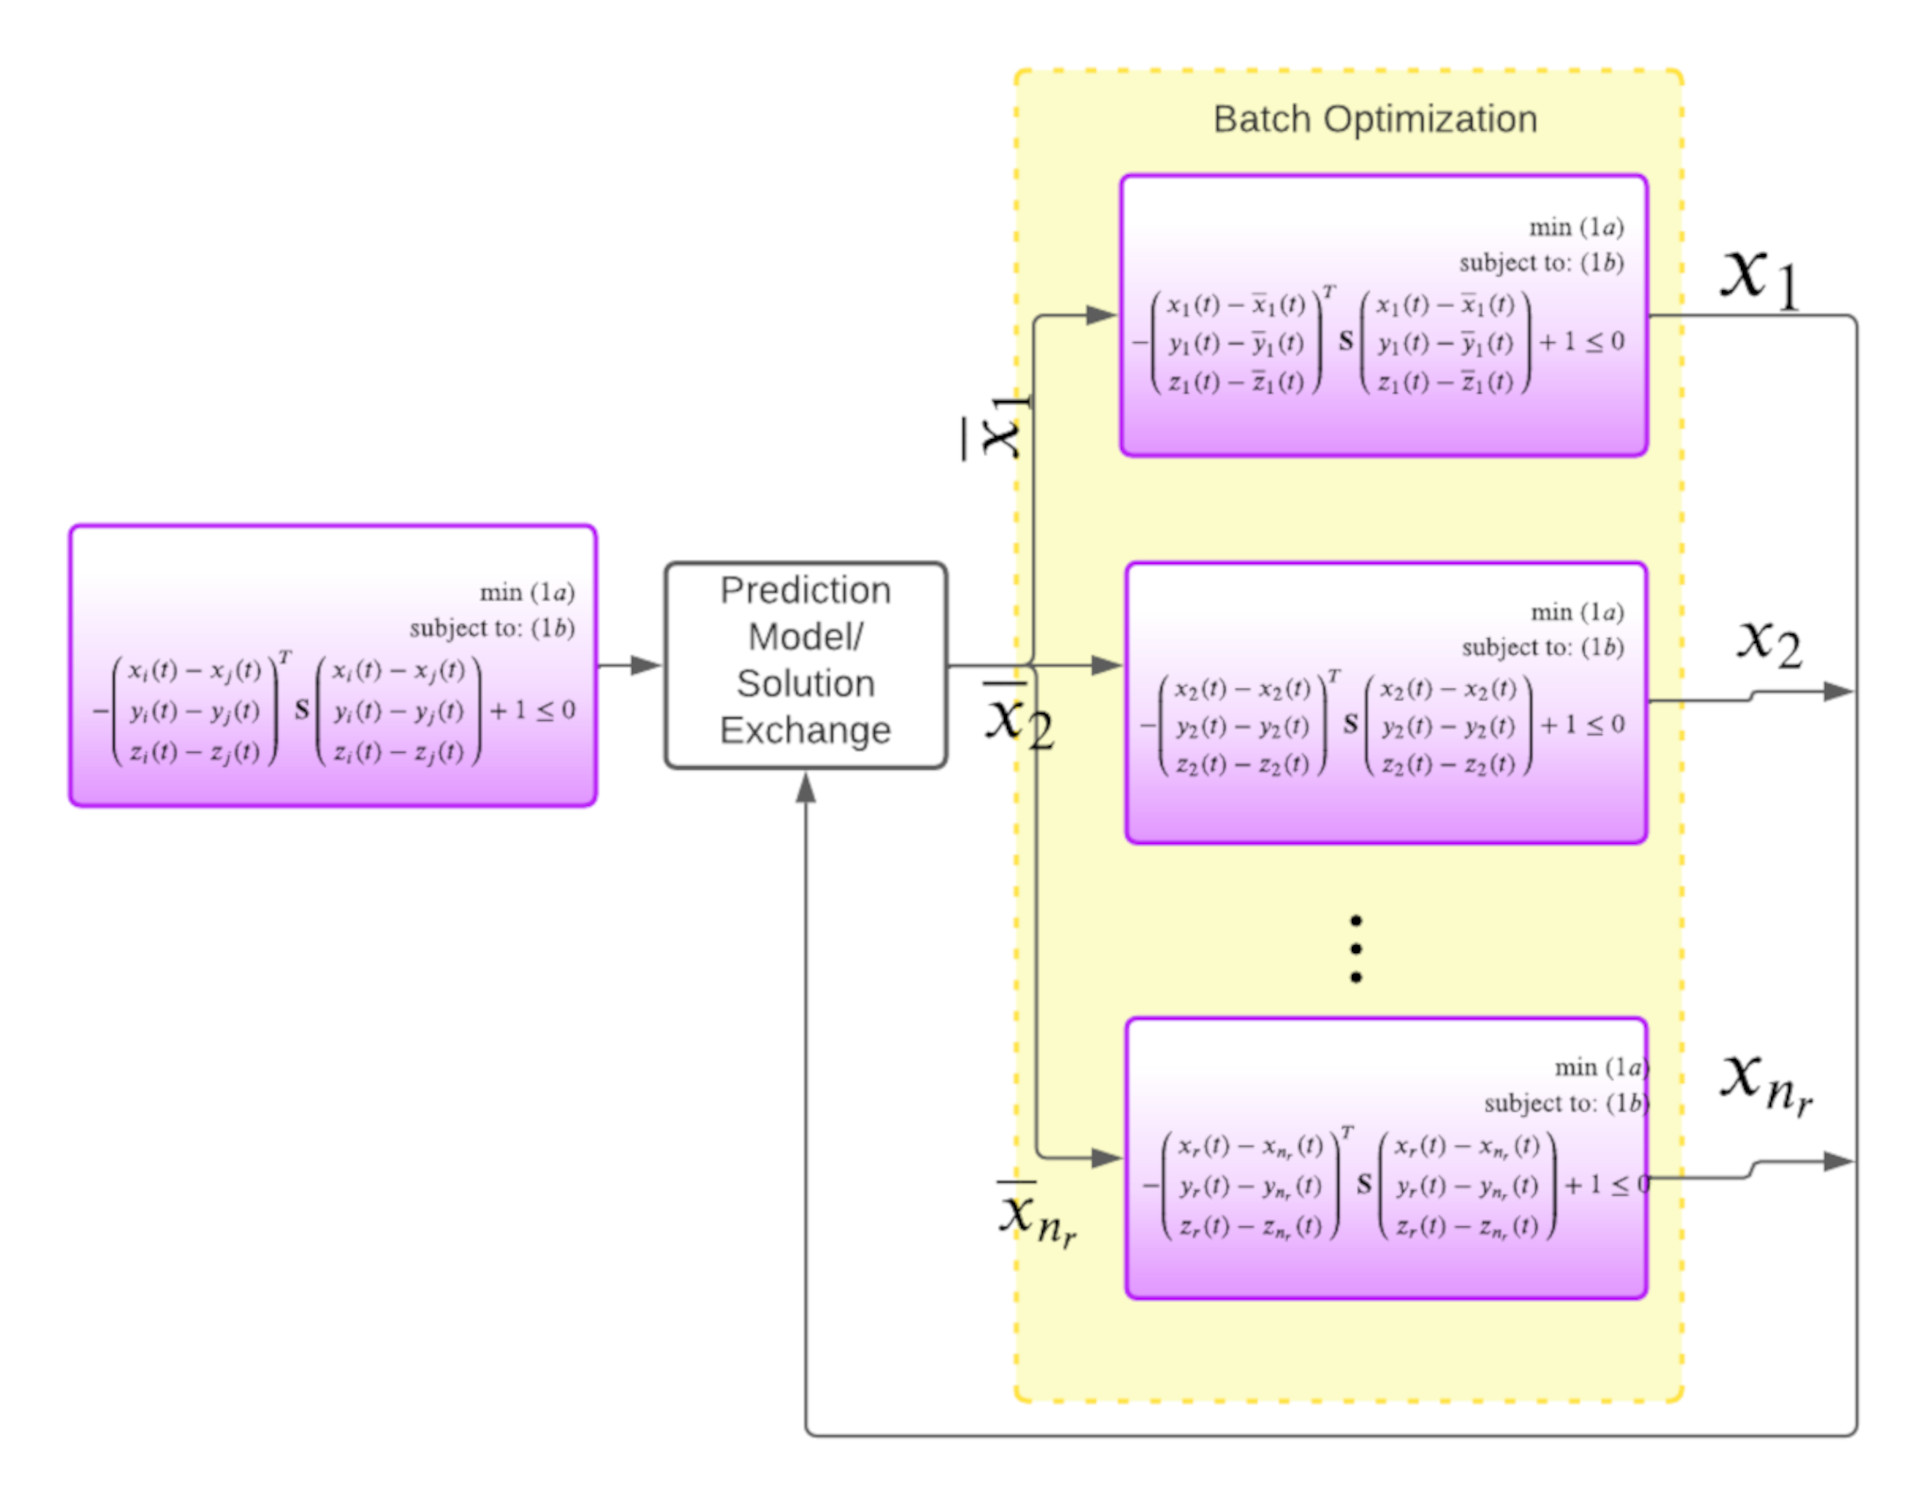
\includegraphics{figures/gpu_mat/pipeline.jpg}} 
    \caption[GPU multi-robot optimizer pipeline]{ Figure shows our approach for breaking the joint optimization (first block) at each iteration into decoupled sub-problems (third group of blocks). Each robot exchanges their current computed trajectories with each other. For the next iteration, robots will use the communicated trajectories to frame their collision avoidance constraints. Thus, in this manner, we can avoid the inter-robot coupling in collision constraints. Our core novelty in this chapter is a batch optimizer that can solve all the decoupled problems in parallel over GPUs. It is also possible to replace the trajectory exchange set-up with a model that predicts the nature of the robot trajectories in the immediate next iteration. Note that we only show the $x$ component of the trajectory purely to maintain clarity in the figure.}
    \label{fig: figure_block_diagram}
\end{figure}

\begin{align}
    \left(\begin{matrix}
    x_i(t)-\overline{x}_j(t)\\
 y_i(t)-\overline{y}_j(t)\\
 z_i(t)-\overline{z}_j(t)\\
 \end{matrix}\right)^T\textbf{S}\left(\begin{matrix}
 x_i(t)-\overline{x}_j(t)\\
 y_i(t)-\overline{y}_j(t)\\
 z_i(t)-\overline{z}_j(t)\\
 \end{matrix}\right)+1 \leq 0
 \label{distributed_coll}
\end{align}

\noindent Note that $(\overline{x}_j(t), \overline{y}_j(t), \overline{z}_j(t) )$ is a known constant in (\ref{distributed_coll}). Fig.\ref{fig: figure_block_diagram} shows how the process of using (\ref{distributed_coll}) to formulate decoupled optimization problems for each robot. Existing works differ in their method of computing the prediction $(\overline{x}_j(t), \overline{y}_j(t), \overline{z}_j(t) )$. The simplest possibility is to set it as the solution obtained in the previous iteration \citep{alonso_mora_nips_multi}, which is what we use in our formulation as well.

\subsubsection{Online DMPC} 
\noindent DMPC approaches are the online variants of the distributed optimization approach. In other words, if we run one iteration of distributed optimization and let each robot move with the computed trajectory, we recover the DMPC works such as \citep{dmpc_carlos}, \cite{dmpc_carlos_2}. This insight also points to the main issue of DMPC. At each control cycle, imagine a robot $i$ receiving information (directly through communications or indirectly through prediction) about the trajectory that the other robot $j$ computed. Then it uses this information to construct collision avoidance constraints in its trajectory optimization set-up. However, robot $j$ will follow the same process and update its trajectory as well. Thus, essentially both robot $i$ and $j$ compute their motion based on outdated information about each other's behavior.

\subsubsection{Batch optimization over CPU Vs GPU}

Parallelization of a batch of optimization problems across CPUs and GPUs operates fundamentally differently, and both classes of approaches have been tried in existing works to speed up multi-robot trajectory optimization. Each CPU core is efficient at handling arbitrary numerical computations, and thus solving a batch of optimizations problems in parallel is conceptually simple. We can solve each problem in a separate thread without needing to make any change in the underlying numerical algebra of the optimizer \citep{aks_behavior_ral22}, \citep{alonso_mora_nips_multi}. As mentioned earlier, the scalability of CPU parallelization is limited by the number of cores (typical 6 in a standard laptop). On the other hand, GPUs have many cores, but these are primarily efficient at parallelizing primitive operations such as matrix-vector and matrix-matrix multiplication.
Moreover, GPUs excel in performing the same primitive operations over many data points. Thus, to fully leverage the compute power of GPUs, it is necessary to modify the underlying numerical aspect of an optimizer to fit the strengths of GPUs. For example, GPU acceleration of Newton's method requires adopting indirect matrix factorization over the more common direct approaches \citep{newton_gpu}. One optimization technique that trivially accelerates over GPUs is Gradient Descent (GD) since it boils down to just matrix-vector multiplication. Authors in \citep{rafaella_gpu} leverage this insight for developing a fast multi-robot trajectory optimization algorithm. One critical issue of \citep{rafaella_gpu} is that the proposed GD is very sensitive to hyper-parameters like weights of the different cost function, learning rate, etc.


    %\caption{Empirical validation of convergence of our optimizer. The figure shows the residual of $\Vert \textbf{F}\boldsymbol{\xi}_{1, i}-\textbf{g}_i\Vert$ averaged over all $i$ (agent index) and across different benchmarks.}

GPUs are designed using threads grouped into blocks, which are themselves organized as grids to parallelize computations for computational efficiency \citep{li_GPUmatmul}. The GPU first tiles an $n \times n$ matrix using $p \times q$ tiles indexed with a 2-dimensional index to multiply large matrices. The output of each tile in the result matrix is independent of other tiles, which allows for parallelization. The parallelized CUDA code uses a block of threads to compute each tile of the result matrix, and to compute the entire result matrix; it uses a $\frac{n}{p} \times \frac{n}{q}$ grid of thread blocks. Many threads and blocks in modern GPUs allow for simultaneous computation of tile outputs, allowing for a many-fold boost in the computation time required for large matrix multiplications. Most off-the-shelf GPU-based libraries have this inbuilt CUDA programming for parallel GPU computations and can be utilized for achieving computational speed-ups in matrix multiplications.


% Our approach in this chapter for solving the batch of distributed sub-problems arising at each iteration of multi-robot trajectory optimization is more sophisticated than a typical GD based optimizer. As, we


% We reduce the operations of batch optimization to solving a set of linear equations (see \eqref{over_2}).\color{black}


\section{Methods}
\subsection{Overview} \label{batch_QP_setup}
\noindent Similar to \citep{alonso_mora_nips_multi}, we break the joint multi-robot trajectory optimization (\ref{cost_multirobot})-(\ref{coll_multirobot}) into decoupled smaller sub-problems at each iteration. This is illustrated in Fig.\ref{fig: figure_block_diagram}. At a conceptual level, this decoupling process can be interpreted in the following manner: the robots communicate among themselves the trajectories they obtained in the previous iteration of the optimizer. Each robot then uses them to independently formulate their collision avoidance constraints. Our work differs from existing works in the way the decoupled problems illustrated in Fig.\ref{fig: figure_block_diagram} is solved. As mentioned before, a trivial approach to solving the sub-problems in parallel CPU threads is not scalable for tens of robots. In contrast, our main idea in this chapter is to develop a GPU accelerated optimizer that can solve a batch of optimization problems in one shot. 

In this sub-section, we aim to provide a succinct mathematical abstraction of our main idea. We discuss a special class of problems that are simple to solve in batch fashion. To this end, consider the following batch of equality constrained QPs, $ i\in \{1,2,...,n_r\}$.

\begin{align}
\min_{\boldsymbol{\xi}_{i}} \Big(\frac{1}{2}\boldsymbol{\xi}^{T}_{i}\overline{\textbf{Q}}\boldsymbol{\xi}_{i} + \overline{\textbf{q}}^{T}_{i}\boldsymbol{\xi}_{i}\Big), \qquad
 \text{st: } \overline{\textbf{A}} \boldsymbol{\xi}_{i} = \overline{\textbf{b}}_{i} \label{over_1}
\end{align}

\noindent In total, there are $n_r$ QPs to be solved, each defined over variable $\boldsymbol{\xi}_i$. The QPs defined in (\ref{over_1}) have a unique structure. The Hessian $\overline{\textbf{Q}}$ and the constrained matrix $\overline{\textbf{A}}$ are shared across the problems and only the vectors $\overline{\textbf{q}}_i$ and $\overline{\textbf{b}}_i$ varies across the batch. This special structure leads to efficient batch solution formulae. To see how, note that each QP in the batch can be reduced to solving the following set of linear equations.

\begin{align}
    \begin{bmatrix}
        \overline{\textbf{Q}} & \overline{\textbf{A}}^{T} \\ 
        \overline{\textbf{A}} & \textbf{0}
    \end{bmatrix} \begin{bmatrix}
        \boldsymbol{\xi}_{i}\\ \boldsymbol{\mu}_{i}
    \end{bmatrix} = \begin{bmatrix}
        \overline{\textbf{q}}_{i} \\ \overline{\textbf{b}}_{i}
    \end{bmatrix}, \qquad \forall i \in \{ 1,2,...,n_{r} \} \label{over_2}
\end{align}

\noindent where $\boldsymbol{\mu}_i$ are the dual optimization variables. Now, it can be observed that the matrix on the left-hand side of (\ref{over_2}) is independent of the batch index $i$, and thus, the solutions for the entire batch can be computed in one shot through \eqref{over_3}.

\begin{align}
\begin{bmatrix} 
\begin{array}{@{}c|c|cc@{}}
\boldsymbol{\xi}_{1} &...& \boldsymbol{\xi}_{n_{r}} \\ \boldsymbol{\mu}_{1} &...& \boldsymbol{\mu}_{n_{r}}
\end{array}
\end{bmatrix} =
    \overbrace{\left (\begin{bmatrix}
        \overline{\textbf{Q}} & \overline{\textbf{A}}^{T} \\ 
        \overline{\textbf{A}} & \textbf{0}
    \end{bmatrix}^{-1}\right )}^{matrix}
\overbrace{\begin{bmatrix}
\begin{array}{@{}c|c|cc@{}}
    \overline{\textbf{q}}_{1} & \overline{\textbf{q}}_{2}& ... & \overline{\textbf{q}}_{n_{r}}  \\
    \overline{\textbf{b}}_1 & \overline{\textbf{b}}_2 & ... & \overline{\textbf{b}}_{n_{r}} 
    \end{array}\end{bmatrix}}^{\text{stacked vectors}},
    \label{over_3}
\end{align}

\noindent where $|$ represents that the columns are stacked horizontally. The batch solution (\ref{over_3}) amounts to multiplying one single matrix with a batch of vectors. Furthermore, the matrix is constant, and its dimension is independent of the number of problems in the batch. Thus, operation (\ref{over_3}) can be trivially parallelized over GPUs using off-the-shelf libraries like JAX \citep{bradbury2020jax}.

\noindent \textbf{How it all fits:} In the next few sub-sections, we will show how the distributed sub-problems of (\ref{cost_multirobot})-(\ref{coll_multirobot}), shown in Fig.\ref{figure1} can be solved efficiently in a batch setting. Specifically, we reformulate these problems in such a way that the most intensive part of their solution process reduces to solving a batch of QPs with the special structure presented in (\ref{over_1}). 

\subsection{Collision Avoidance in Polar Form}
\noindent An important building block of our approach is rephrasing the collision avoidance constraints into the following polar representation from \citep{aks_ral21}, \citep{rastgar2020novel}.

\begin{align}
\textbf{f}_{c}(x_{i}(t),y_{i}(t)) = 
\left \{ \begin{array}{lcr}
x_{i}(t) - \overline{x}_{j}(t) - ad_{ij}(t)\sin{\beta_{ij}(t)}\cos{\alpha_{ij}(t)} \\
y_{i}(t) - \overline{y}_{j}(t) - ad_{ij}(t)\sin{\beta_{ij}(t)}\sin{\alpha_{ij}(t)} \\
z_{i}(t) - \overline{z}_{j}(t) - bd_{ij}(t)\cos{\beta_{ij}(t)}
\end{array} \right \},  \qquad  d_{ij}(t) \geq 1,
\label{fc} 
\end{align}

\noindent where $\alpha_{ij}(t), \beta_{ij}(t), d_{ij}(t)$  are unknown variables that will be computed by the optimizer along with each robot's trajectory. Physically, $\alpha_{ij}(t)$ and $\beta{ij}(t)$ represent the 3D solid angle of the line-of-sight connecting robot $i$ and $j$ based on the predicted motion of the latter. The variable $d_{ij}(t)$ is the ratio of the length of the line-of-sight vector with minimum safe distance $\sqrt{a^2+a^2+b^2}$ (see \citep{aks_ral21}).

\subsection{Proposed Reformulated Distributed Problem}
\noindent Using (\ref{fc}), we can reformulate the distributed sub-problems presented in Fig.\ref{figure1} for the $i^{th}$ robot in the following manner. We reiterate that $(\overline{x}_j(t), \overline{y}_j(t), \overline{z}_j(t)), \forall j\neq i $ is known based on the prediction of the trajectories of other robots.

\begin{subequations}
\begin{align}
\min_{ \scalebox{0.8}{$ x_{i}(t), y_{i}(t), z_{i}(t), d_{ij}(t),
\alpha_{ij}(t), \beta_{ij}(t)  $}}
\sum_t \Big(\ddot{x}^2_{i}(t)+\ddot{y}^2_{i}(t) + \ddot{z}^2_{i}(t) \Big), \label{acc_cost_reform}\\
 %\Tilde{\psi}(t)=\psi(t) \label{reformulate_psi}\\
\Big(x_i(t_0), \dot{x}_i(t_0), \ddot{x}_i(t_0), y_i(t_0), \dot{y}_i(t_0), \ddot{y}_i(t_0), z_i(t_0), \dot{z}_i(t_0), \ddot{z}_i(t_0)) = \textbf{b}_{o, i}, \forall i \label{initial_boundary_cond_reform} \\
\Big(x_i(t_f), \dot{x}_i(t_f), \ddot{x}_i(t_f), y_i(t_f), \dot{y}_i(t_f), \ddot{y}_i(t_f), z_i(t_f), \dot{z}_i(t_f), \ddot{z}_i(t_f)) = \textbf{b}_{f, i}, \forall i \label{final_boundary_cond_reform} \\
\textbf{f}_{c} \hspace{-0.1cm}: \hspace{-0.1cm}\left \{ \begin{array}{lcr}
x_{i}(t)-\overline{x}_{j}(t) -ad_{ij}(t)\sin{\beta_{ij}(t)}\cos{\alpha_{ij}}(t)\\
y_{i}(t)-\overline{y}_{j}(t) 
-ad_{ij}(t)\sin{\beta_{ij}(t)}\sin{\alpha_{ij}(t)} \\
z_{i}(t)-\overline{z}_{j}(t) -bd_{ij}(t)\cos{\beta_{ij}(t)}
\end{array} \right \} \label{coll_con} \\% \right \}
 d_{ij}(t) \geq 1, \qquad \forall t, j, \{j| j\in \{1,2,...,n_{r}\}, j \neq  i\} \label{collision_reform}
\end{align}
\end{subequations}

\subsubsection{Finite Dimensional Representation}
\noindent Optimization (\ref{acc_cost_reform})-(\ref{collision_reform}) is expressed in terms of functions and thus has the so called infinite dimensional representaton. To obtain a finite-dimensional form, we assume some parametric form for this functions. For
different $d_{ij}(t), \alpha_{a_{ij}}(t), \beta_{ij}(t) $, we assume a way-point paramterization. That is, these functions are represented through values at discrete time instants. The trajectories along each motion axis are represented as following polynomials.

\begin{equation}
\begin{bmatrix}
x_{i}(t_1)\\
x_{i}(t_2)\\
\vdots\\
x_{i}(t_{n_{p}})
\end{bmatrix} =\textbf{P} \textbf{c}_{x,i}, \qquad
\begin{bmatrix}
\dot{x}_{i}(t_1)\\
\dot{x}_{i}(t_2)\\
\vdots\\
\dot{x}_{i}(t_{n_{p}})
\end{bmatrix} = \dot{\textbf{P}}\textbf{c}_{x,i}, \qquad
\begin{bmatrix}
\ddot{x}_{i}(t_1)\\
\ddot{x}_{i}(t_2)\\
\vdots\\
\ddot{x}_{i}(t_{n_{p}})
\end{bmatrix} = \ddot{\textbf{P}}\textbf{c}_{x,i}.
\label{param}
\end{equation}

\noindent Similar expressions as (\ref{param}) can be written for the $y, z$ component of the trajectory as well. The matrix $\textbf{P}$ is formed with time dependent polynomial basis functions. Using (\ref{param}), we can re-write (\ref{acc_cost_reform})-(\ref{collision_reform}) in the following matrix form. 

\begin{subequations}
\begin{align}
 \min_{\boldsymbol{\xi}_{1,i}, \boldsymbol{\xi}_{2,i}, \boldsymbol{\xi}_{3,i}, \boldsymbol{\xi}_{4,i}} \Big(\frac{1}{2}\boldsymbol{\xi}_{1,i}^T\textbf{Q}\boldsymbol{\xi}_{1,i} \Big)\label{cost_matrix_form},  \\
  \textbf{A}_{eq}\boldsymbol{\xi}_{1,i} = \textbf{b}_{eq},   \label{eq_matrix_form}\\
  \textbf{F}\boldsymbol{\xi}_{1,i} = \textbf{g}_{i}(\boldsymbol{\xi}_{2,i},\boldsymbol{\xi}_{3,i}, \boldsymbol{\xi}_{4,i} ) \label{non_convex_equality_matrix-form},\\
 \boldsymbol{\xi}_{4,i}\geq \textbf{1}, \label{d_bound_matrix_form}
\end{align}
\end{subequations}

\noindent where, $\boldsymbol{\xi}_{1,i} = (\textbf{c}_{x,i}, \textbf{c}_{y,i}, \textbf{c}_{z,i}) $, $\boldsymbol{\xi}_{2,i} = \boldsymbol{\alpha}_{ij}$,  $\boldsymbol{\xi}_{3,i} = \boldsymbol{\beta}_{ij}$ and $\boldsymbol{\xi}_{4,i} = \textbf{d}_{ij}$. Note that $\boldsymbol{\alpha}_{ij}$ is formed by stacking $\alpha_{ij}(t)$ at different time instants. Similar construction is followed for other elements in $\boldsymbol{\xi}_2, \boldsymbol{\xi}_3$. The matrix $\textbf{Q}$ is block diagonal matrix with $\ddot{\textbf{P}}^T\ddot{\textbf{P}}$ as main diagonal block. The affine constraint \eqref{eq_matrix_form} is a matrix representation of the initial and final boundary conditions \eqref{initial_boundary_cond_reform}-\ref{final_boundary_cond_reform}. The matrix $\textbf{A}_{eq}$ and vector $\textbf{b}_{eq}$ is constructed in the following manner.

\begin{align}
    \textbf{A}_{eq} = \begin{bmatrix}
    \textbf{A} & \textbf{0}\\
    \textbf{0} & \textbf{A}\\
    \end{bmatrix}, \textbf{A}_{eq} = \begin{bmatrix}
    \textbf{P}_1|\dot{\textbf{P}}_1| \ddot{\textbf{P}}_1| \textbf{P}_{-1}|\ddot{\textbf{P}}_{-1} \ddot{\textbf{P}}_ {-1}
    \end{bmatrix}^T, \textbf{b}_{eq} = \begin{bmatrix}
    \textbf{b}_{0, i}\\
    \textbf{b}_{f, i},\\
    \end{bmatrix}
\end{align}

\noindent where, $\textbf{P}_{1}, \dot{\textbf{P}}_{1}, \ddot{\textbf{P}}_{1}, \textbf{P}_{-1}, \dot{\textbf{P}}_{-1}, \ddot{\textbf{P}}_{-1}$ represents the first and last elements of the corresponding matrices.

\noindent Matrix $\textbf{F}$ and vector $\textbf{g}_{i}$ defining constraints (\ref{collision_reform}) are constructed as 

\begin{align}
\textbf{F} = \begin{bmatrix} 
\textbf{F}_{o} & \textbf{0} & \textbf{0} \\
 \textbf{0} & \textbf{F}_{o} & \textbf{0} \\
   \textbf{0}  & \textbf{0} & \textbf{F}_{o} 
\end{bmatrix}
\qquad 
\textbf{g}_{i} = 
\begin{bmatrix}
\textbf{g}_{x,{i}}(\boldsymbol{\xi}_{2,i}, \boldsymbol{\xi}_{3,i}, \boldsymbol{\xi}_{4,i}) \\
\textbf{g}_{y,{i}}(\boldsymbol{\xi}_{2,i}, \boldsymbol{\xi}_{3,i}, \boldsymbol{\xi}_{4,i}) \\
\textbf{g}_{z,{i}}(\boldsymbol{\xi}_{2,i}, \boldsymbol{\xi}_{3,i}, \boldsymbol{\xi}_{4,i})
\end{bmatrix}
\label{f_g_matrix}
\end{align}

\noindent where,

\begin{align}
\textbf{g}_{x,{i}} =
\overline{\textbf{x}}_{j} 
+ a
\textbf{d}_{ij} \sin{\boldsymbol{\beta}_{ij}}\cos{\boldsymbol{\alpha}_{ij}}, \forall j
 , \qquad
\textbf{g}_{y,{i}}=
\overline{\textbf{y}}_{j} + a \textbf{d}_{ij}\sin{\boldsymbol{\beta}_{ij}}\sin{\boldsymbol{\alpha}_{ij}} , \forall j,
\qquad
\textbf{g}_{z, i}=
\overline{\textbf{z}}_{j} + b \textbf{d}_{ij}\cos{\boldsymbol{\beta}_{ij}}, \forall j
\end{align}

\noindent and $\textbf{F}_{o}$ is formed by vertically stacking $\textbf{P}$, $n_r-1$ times. The vectors $\overline{\textbf{x}}_j,\overline{\textbf{y}}_j, \overline{\textbf{z}}_j$ are formed by stacking $\overline{x}_j(t), \overline{y}_j(t), \overline{z}_j(t) $ at different time instants.

\begin{remark}\label{i_th_agent_remark}

The subscript $i$ signifies that \eqref{cost_matrix_form}-\eqref{non_convex_equality_matrix-form} is constructed for the $i^{th}$ agent.

\end{remark}

\begin{remark}\label{non_convexity_roll}
All the non-convexity in optimization (\ref{cost_matrix_form})-(\ref{d_bound_matrix_form}) is rolled into the equality constraint (\ref{non_convex_equality_matrix-form})
\end{remark}

\begin{remark} \label{remark_constant_matrix}
The matrices $\textbf{A}_{eq}, \textbf{F}$ in optimization (\ref{cost_matrix_form})-(\ref{d_bound_matrix_form}) is independent of the robot index. In other words, these matrices remain the same irrespective of the which sub-problems shown in Fig.\ref{figure1}, we are solving.
\end{remark}

\noindent Remark \ref{remark_constant_matrix} sheds light behind our motivation of presenting the elaborate reformulations of the collision avoidance constraints. In fact, on the surface, our chosen representation (\ref{fc}) seems substantially more complicated than the conventional form (\ref{coll_multirobot}) based on the Euclidean norm. In the next sub-section, we present an optimizer that can leverage the insights presented in Remark \ref{remark_constant_matrix}. More precisely, we will show that the due to the matrices $\textbf{A}_{eq}, \textbf{F}$ being independent of the robot index $i$, the  most intensive part of solving (\ref{cost_matrix_form})-(\ref{d_bound_matrix_form}) reduces to the batch QP structure presented in sub-section \ref{batch_QP_setup}

\subsection{Augmented Lagrangian and Alternating Minimization}
\noindent Our proposed optimizer for (\ref{cost_matrix_form})-(\ref{d_bound_matrix_form}) relies on relaxing the non-convex equality constraints (\ref{non_convex_equality_matrix-form}) as $l_2$ penalties and incorporating them into the cost function in the following manner.

\begin{align}
 \min_{\boldsymbol{\xi}_{1,i},\boldsymbol{\xi}_{2,i},\boldsymbol{\xi}_{3,i}, \boldsymbol{\xi}_{4,i} } 
 \Big(\frac{1}{2}\boldsymbol{\xi}_{1,i}^T\textbf{Q}\boldsymbol{\xi}_{1,i} 
 - \langle\boldsymbol{\lambda}_{i}, \boldsymbol{\xi}_{1,i}\rangle 
 +\frac{\rho}{2}\left\Vert \textbf{F} \boldsymbol{\xi}_{1,i}  
 -\textbf{g}_{i}(\boldsymbol{\xi}_{2,i},\boldsymbol{\xi}_{3,i}, \boldsymbol{\xi}_{4,i}) \right \Vert_2^2 \Big) %\nonumber \\
 \label{reform_bergman}
 \end{align}
 
\noindent As the residual of the constraint term is driven to zero, we recover the solution to the original problem. To this end, the parameter $\boldsymbol{\lambda}_{i}$, known as the Lagrange multiplier, plays an important part. Its role is to appropriately weaken the effect of the primary cost function so that the optimizer can focus on minimizing the constraint residual \citep{admm_neural}. The parameter $\rho$ is a scalar and is typically constant. However, it is possible to increase or decrease it depending on the magnitude of the constraint residual at each iteration of the optimizer.
 
The relaxation of non-convex equality constraints, as augmented Lagrangian (AL) cost, is extensively used in non-convex optimization \citep{admm_non_convex_1}, \citep{admm_non_convex_2}. However, what differentiates our use of AL from existing works is how we minimize (\ref{reform_bergman}). Typical approaches towards non-convex optimization are based on first (and sometimes second) order Taylor Series expansion of the non-convex costs or constraints. In contrast, we adopt an Alternating Minimization (AM) based approach, wherein at each iteration, we minimize only one of the variable blocks amongst $\boldsymbol{\xi}_{1, i}, \boldsymbol{\xi}_{2, i}, \boldsymbol{\xi}_{3, i}, \boldsymbol{\xi}_{4, i}  $ while others are held constant at specific values. In the next section, we present the various steps of our AM optimizer and highlight how it never requires any linearization of cost or constraints. Moreover, we show how the AM steps naturally lead to a simple yet efficient batch update rule using which we can solve (\ref{cost_matrix_form})-(\ref{d_bound_matrix_form}) for all the robots in one shot.



% \begin{enumerate}
% \item \textbf{Initialization:}  Initialize ${^{k}}\boldsymbol{\xi}_{2,i}$, ${^{k}}\boldsymbol{\xi}_{3,i}$ and ${^{k}}\boldsymbol{\xi}_{4,i}$ values at iteration $k$.
% \item \textbf{Computing ${^{k+1}}\boldsymbol{\xi}_{1,i}$:} 
% The optimization problem \eqref{reform_bergman} with respect to $\boldsymbol{\xi}_{1,i}$ can be rephrased as
% \begin{align}
% {^{k+1}}\boldsymbol{\xi}_{1,i} = \min_{\boldsymbol{\xi}_{1,i}}\Big(\frac{1}{2}\boldsymbol{\xi}_{1,i}^T\textbf{Q}\boldsymbol{\xi}_{1,l} 
%  - \langle {^{k}}\boldsymbol{\lambda}_{i}, \boldsymbol{\xi}_{1,i}\rangle 
%  +\frac{\rho}{2}\left\Vert \textbf{F}\boldsymbol{\xi}_{1,i}  
%  -\textbf{g}_{i}({^{k}}\boldsymbol{\xi}_{2,i},{^{k}}\boldsymbol{\xi}_{3,i}, {^{k}}\boldsymbol{\xi}_{4,i}) \right \Vert_2^2 
%   \Big )
%   , \qquad
%   \textbf{A}_{eq}\boldsymbol{\xi}_1 = \textbf{b}_{eq} \label{zeta_1_sepration_1}
%  \end{align}
%  \item \textbf{Computing ${^{k+1}}\boldsymbol{\xi}_{2,i}$:}
% After computing ${^{k+1}}\boldsymbol{\xi}_{1,i}$, we want to minimize the optimization problem \eqref{reform_bergman} with respect to $\boldsymbol{\xi}_{2,i}$. Thus, we have
% \begin{align}
% {^{k+1}}\boldsymbol{\xi}_{2,i}  = \min_{\boldsymbol{\xi}_{2,i}}\Big( \frac{\rho}{2}\left\Vert \textbf{F}^{k+1} \boldsymbol{\xi}_{1,i}  
%  -\textbf{g}_{i}(\boldsymbol{\xi}_{2,i}, ^{k}\boldsymbol{\xi}_{3,i}, ^{k}\boldsymbol{\xi}_{4,i}) \right \Vert_2^2 \Big) 
%  \label{compute_ze_3}
% \end{align}

% \item \textbf{Computing ${^{k+1}}\boldsymbol{\xi}_{3,i}$:}
% Considering updated $\boldsymbol{\xi}_{1,i}$ and $\boldsymbol{\xi}_{2,i}$, we are interested in solving  \eqref{reform_bergman} with respect to ${^{k+1}}\boldsymbol{\xi}_{3,i}$. So, we can rewrite \eqref{reform_bergman} as  
% \begin{align}
% {^{k+1}}\boldsymbol{\xi}_{3,i}= \min_{\boldsymbol{\xi}_{3,i}}\Big(\frac{\rho}{2}\left\Vert \textbf{F}^{k+1} \boldsymbol{\xi}_{1,i} - \textbf{g}_{i}(^{k+1}\boldsymbol{\xi}_{2,i},\boldsymbol{\xi}_{3,i}, ^{k}\boldsymbol{\xi}_{4,i}) \right \Vert_2^2 \Big)
%  \label{compute_ze_44}
% \end{align}

% \item \textbf{Computing ${^{k+1}}\boldsymbol{\xi}_{4,i}$:}
% Considering all computed variables in previous steps, we solve \eqref{reform_bergman} with respect to ${^{k+1}}\boldsymbol{\xi}_{4,i}$. So, we have
% \begin{align}
% {^{k+1}}\boldsymbol{\xi}_{4,i}= \min_{\boldsymbol{\xi}_{4,i}}\Big(\frac{\rho}{2}\left\Vert \textbf{F}^{k+1} \boldsymbol{\xi}_{1,i} - \textbf{g}_{i}(^{k+1}\boldsymbol{\xi}_{2,i},^{k+1}\boldsymbol{\xi}_{3,i}, \boldsymbol{\xi}_{4,i}) \right \Vert_2^2 \Big)
%  \label{compute_ze_4}
% \end{align}

% \item \textbf{Updating Lagrange multipliers ${^{k+1}}\boldsymbol{\lambda}_{i}$:} Finally, we update the Lagrange multiplier $\boldsymbol{\lambda}_{i}$.
% \end{enumerate}



\begin{algorithm*}[!h]
%\centering
 \caption{Alternating Minimization (AM) based solution for the $i^{th}$ Sub-Problem}\label{algo_batch}
   % \begin{algorithmic}[1]   
    \textbf{Initialize} ${^{k}}\boldsymbol{\xi}_{2,i}$, ${^{k}}\boldsymbol{\xi}_{3,i}$ and ${^{k}}\boldsymbol{\xi}_{4,i}$ values at iteration $k=0$.
   \textbf{while} $k\leq \text{max iteration}$ \text{ or till norm of the residuals are below some threshold}
\begin{align}
{^{k+1}}\boldsymbol{\xi}_{1,i} = \min_{\boldsymbol{\xi}_{1,i}}\Big(\frac{1}{2}\boldsymbol{\xi}_{1,i}^T\textbf{Q}\boldsymbol{\xi}_{1,l} 
 - \langle {^{k}}\boldsymbol{\lambda}_{i}, \boldsymbol{\xi}_{1,i}\rangle 
 +\frac{\rho}{2}\left\Vert \textbf{F}\boldsymbol{\xi}_{1,i}  
 -\textbf{g}_{i}({^{k}}\boldsymbol{\xi}_{2,i},{^{k}}\boldsymbol{\xi}_{3,i}, {^{k}}\boldsymbol{\xi}_{4,i}) \right \Vert_2^2 
  \Big )
  , \qquad
  st.\textbf{A}_{eq}\boldsymbol{\xi}_1 = \textbf{b}_{eq} \label{zeta_1_sepration_1}
 \end{align}
\begin{align}
{^{k+1}}\boldsymbol{\xi}_{2,i}  = \min_{\boldsymbol{\xi}_{2,i}}\Big( \frac{\rho}{2}\left\Vert \textbf{F}^{k+1} \boldsymbol{\xi}_{1,i}  
 -\textbf{g}_{i}(\boldsymbol{\xi}_{2,i}, ^{k}\boldsymbol{\xi}_{3,i}, ^{k}\boldsymbol{\xi}_{4,i}) \right \Vert_2^2 \Big) 
 \label{compute_ze_2}
\end{align}
\begin{align}
{^{k+1}}\boldsymbol{\xi}_{3,i}= \min_{\boldsymbol{\xi}_{3,i}}\Big(\frac{\rho}{2}\left\Vert \textbf{F}^{k+1} \boldsymbol{\xi}_{1,i} - \textbf{g}_{i}(^{k+1}\boldsymbol{\xi}_{2,i},\boldsymbol{\xi}_{3,i}, ^{k}\boldsymbol{\xi}_{4,i}) \right \Vert_2^2 \Big)
 \label{compute_ze_3}
\end{align}
\begin{align}
{^{k+1}}\boldsymbol{\xi}_{4,i}= \min_{\boldsymbol{\xi}_{4,i}}\Big(\frac{\rho}{2}\left\Vert \textbf{F}^{k+1} \boldsymbol{\xi}_{1,i} - \textbf{g}_{i}(^{k+1}\boldsymbol{\xi}_{2,i},^{k+1}\boldsymbol{\xi}_{3,i}, \boldsymbol{\xi}_{4,i}) \right \Vert_2^2 \Big)
 \label{compute_ze_4}
\end{align}
\begin{align}
{^{k+1}}\boldsymbol{\lambda}_{i}={^{k}}\boldsymbol{\lambda}_{i} - \rho( \textbf{F} \hspace{0.1cm} ^{k+1}\boldsymbol{\xi}_{1,i} 
 -\textbf{g}_{i}(^{k+1}\boldsymbol{\xi}_{2,i} , ^{k+1}\boldsymbol{\xi}_{3,i},^{k+1}\boldsymbol{\xi}_{4,i} ))\textbf{F}
\label{update_lambda_1} 
\end{align}
%\EndWhile
 Return ${^{k+1}}\overline{\boldsymbol{\xi}}_{1, i}$
%\end{algorithmic}
\end{algorithm*}


\subsection{AM Steps and Batch Update Rule}
\noindent Our AM based optimizer for minimizing (\ref{reform_bergman}) subject to \eqref{eq_matrix_form}-\eqref{d_bound_matrix_form} is presented in Algorithm \ref{algo_batch}. Here, the left superscript $k$ is used to track the values of the variable across iteration. For example, ${^k}\boldsymbol{\xi}_{2, i}$ denotes the value of this respective variable at iteration $k$.

The Algorithm begins (line 1) by providing the initial guesses for $\boldsymbol{\xi}_{2, i}, \boldsymbol{\xi}_{3, i}, \boldsymbol{\xi}_{4, i}$. The main optimizer iterations run within the while loop for the specified max iteration limit or till the constraint residuals are a below specified threshold. Each step within the while loop involves solving a convex optimization over just one variable block. We present a more detailed analysis of each of the steps next.

\subsubsection{Analysis}

\noindent \textbf{Step \eqref{zeta_1_sepration_1}:} This optimization is a convex QP
with a similar structure as \eqref{over_1} with 

\begin{align}
\overline{\textbf{Q}}= \textbf{Q} + \rho \textbf{F}^{T}\textbf{F},\qquad
\overline{\textbf{q}}_{i} =  -{^k}\boldsymbol{\lambda}_{i} 
-( \rho\textbf{F}^{T}\textbf{g}_{i}({^k}\boldsymbol{\xi}_{2,i},{^k}\boldsymbol{\xi}_{3,i}, {^k}\boldsymbol{\xi}_{4,i}))^{T}
\label{zeta_1_sepration_3}.
 \end{align}

\noindent Thus, we can easily solve (\ref{zeta_1_sepration_1}) for all the robots in parallel to obtain $(\boldsymbol{\xi}_{1, 1}, \boldsymbol{\xi}_{1, 2}, \boldsymbol{\xi}_{1, 3} , \dots, \boldsymbol{\xi}_{1, n_{r}} ) $ in one shot. The exact solution update is given by \eqref{over_3}.

\noindent For a constant $\rho$, the inverse of $\overline{\textbf{Q}}$ needs to be obtained only once irrespective of the number of robots. Thus, the complexity of the batch solution of all the sub-problems stems purely from obtaining the matrix-matrix products in  \eqref{over_3} and  $\textbf{F}^T\textbf{g}_i, \forall i$. We can formulate the latter also as one large matrix-matrix product in the following manner.

\begin{align} 
   \textbf{F}^T( \overbrace{\begin{bmatrix}
    \textbf{g}_1|\textbf{g}_2|\dots|\textbf{g}_{n_r}
    \end{bmatrix}}^{\textbf{G}})^T
\end{align}

\noindent The dimension of $\textbf{F}$, $\textbf{g}_i$ and $\textbf{G}$ is $( (n_r-1)*n_p) \times 3n_v$, $((n_r-1)*n_p)\times 1$, and  $((n_r-1)*n_p)\times n_r$ respectively. For convenience, we recall that $n_r, n_p, n_v$ represents the number of robots, planning steps and coefficients of the trajectory polynomial (along each axis) respectively. Thus, the row-dimension of $\textbf{F}$ and $\textbf{G}$  increases linearly with $n_r$.



\noindent \textbf{Step \eqref{compute_ze_2}:} The variable ${^{k+1}}\boldsymbol{\xi}_{1, i}$  computed in the previous step and \eqref{param} can be used to fix the position trajectory ${^{k+1}}\boldsymbol{x}_{i}$,  ${^{k+1}}\boldsymbol{y}_{i}$, ${^{k+1}}\boldsymbol{z}_{i}$ at the $(k+1)^{th}$ iteration. Thus, optimization \eqref{compute_ze_2} reduces the following form


% which in turn allows us to treat each element of $\boldsymbol{\xi}_{2, i}$ namely $\boldsymbol{\alpha}_{ij}, \boldsymbol{\beta}_{ij}$ as decoupled from each other. Thus, \eqref{compute_ze_2} reduces to $(n_{r}-1)*n_p$ decoupled problems with the following form.

%  \overbrace{
%   {^{k+1}}\textbf{z}_{i} -  \textbf{z}_{j}
%  }^{{^{k+1}}\boldsymbol{\Tilde{z}}_{i}}
%  -b{^{k}}\textbf{d}_{ij}\cos{\boldsymbol{\beta}_{ij}}
 

%\begin{equations}
\begin{align}
\forall i, j, \qquad {^{k+1}}\boldsymbol{\alpha}_{ij} =   \min_{\boldsymbol{\alpha}_{ij}} 
\frac{\rho}{2} 
\left\Vert  \begin{matrix}
 \overbrace{  
  {^{k+1}}\textbf{x}_{i} - \overline{\textbf{x}}_{j}
}^{{^{k+1}}\boldsymbol{\Tilde{x}}_{i}}
 -a{^{k}} \textbf{d}_{ij} \sin{\boldsymbol{\beta}_{ij}}\cos{\boldsymbol{\alpha}_{ij}} 
\\
 \overbrace{
  {^{k+1}}\textbf{y}_{i} -  \overline{\textbf{y}}_{j}
 }^{{^{k+1}}\boldsymbol{\Tilde{y}}_{i}}
 -a{^{k}}\textbf{d}_{ij}\sin{\boldsymbol{\beta}_{ij}}\sin{\boldsymbol{\alpha}_{ij}} \\
 \end{matrix}
 \right \Vert_2^2 
 \label{compute_zeta_22}  
 \end{align}
 %\end{equation}
 
 \noindent where $\overline{\textbf{x}}_{j}, \overline{\textbf{y}}_{j}$ is formed by stacking $\overline{x}_j(t), \overline{y}_j(t) $ at different time instants.

Although \eqref{compute_zeta_22}  is a seemingly non-convex problem but it has a few favorable computational structures. First, for a fixed position trajectory ${^{k+1}}\boldsymbol{x}_{i}$,  ${^{k+1}}\boldsymbol{y}_{i}$, ${^{k+1}}\boldsymbol{z}_{i}$, we can treat each element of $\boldsymbol{\alpha}_{ij}$ as independent from each other. Thus , \eqref{compute_zeta_22} reduces to $(n_{r}-1)*n_p$ decoupled problems. Second, the solution can be obtained by purely geometrical intuition; $\boldsymbol{\alpha}_{ij}$ is simply one part of the 3D solid-angle of the line-of-sight connecting the $i^{th}$ robot and the predicted trajectory of $j^{th}$ agent. The exact solution update is given by the following. 

\begin{align}
 {^{k+1}}\boldsymbol{\xi}_{2, i} = {^{k+1}}\boldsymbol{\alpha}_{ij} = \arctan2 ({^{k+1}}\boldsymbol{\Tilde{y}}_{i}, {^{k+1}}\boldsymbol{\Tilde{x}}_{i}),
\label{alpha_sol}
\end{align}

\noindent \textbf{Step \eqref{compute_ze_3}:} Following the exact same reasoning as the previous step \eqref{compute_ze_2}, we have the following solution update rule for $\boldsymbol{\xi}_{3, i}$:

 \begin{align}
\boldsymbol{\xi}_{3, i}{^{k+1}} = {^{k+1}}\boldsymbol{\beta}_{ij} = \arctan2(\frac{{^{k+1}}\boldsymbol{\Tilde{x}}_{i}}{a \cos{{^{k+1}}\boldsymbol{\alpha}_{ij}}}, \frac{{^{k+1}}\boldsymbol{\Tilde{z}}_{i}}{b} )
\label{beta_sol}
 \end{align}
 

\noindent \textbf{Step ${^{k+1}}\boldsymbol{\xi}_{4,i}$:} Similar to the last two steps, each element of $\boldsymbol{\xi}_{4, i} = \textbf{d}_{ij}$ once the position trajectory ${^{k+1}}\boldsymbol{x}_{i}$,  ${^{k+1}}\boldsymbol{y}_{i}$, ${^{k+1}}\boldsymbol{z}_{i}$ is fixed. Thus, \eqref{compute_ze_4} can be broken down into $(n_r-1)*n_p$ parallel problems of the  following form.  



\begin{align}
{^{k+1}}\boldsymbol{\xi}_{4, i} = {^{k+1}}\textbf{d}_{ij} =   \min_{\textbf{d}_{ij}\geq 1} 
\frac{\rho}{2} 
\left\Vert  \begin{matrix}
 \overbrace{  
  {^{k+1}}\textbf{x}_{i} - \textbf{x}_{j}
}^{{^{k+1}}\boldsymbol{\Tilde{x}}_{i}}
 -a\textbf{d}_{ij} \sin{{^{k+1}}\boldsymbol{\beta}_{ij}}\cos{{^{k+1}}\boldsymbol{\alpha}_{ij}} 
\\
 \overbrace{
  {^{k+1}}\textbf{y}_{i} -  \textbf{y}_{j}
 }^{{^{k+1}}\boldsymbol{\Tilde{y}}_{i}}
 -a\textbf{d}_{ij}\sin{\boldsymbol{{^{k+1}}\beta}_{ij}}\sin{{^{k+1}}\boldsymbol{\alpha}_{ij}} \\
  \overbrace{
  {^{k+1}}\textbf{z}_{i} -  \textbf{z}_{j}
 }^{{^{k+1}}\boldsymbol{\Tilde{z}}_{i}}
 -b\textbf{d}_{ij}\cos{{^{k+1}}\boldsymbol{\beta}_{ij}}
 \end{matrix}
 \right \Vert_2^2 
 \label{compute_zeta_42}  
 \end{align}

Each optimization in \eqref{compute_zeta_42} is a single variable QP with simple bound constraints. We first obtain the symbolic formulae for the unconstrained version and then clip the resulting solution to $[0 \hspace{0.1cm} 1 ] $.

\begin{remark}\label{matrix_inversion_free_solution}
Evaluating \eqref{alpha_sol}, \eqref{beta_sol} and the solution of \ref{compute_zeta_42} requires no matrix factorization/inverse or even matrix-matrix products. We just need element-wise operation that can obtained for all the sub-problems in one shot. In other words, we obtain $(\boldsymbol{\xi}_{2, 1}, \boldsymbol{\xi}_{2, 2}, \dots \boldsymbol{\xi}_{2, n_r})$, $(\boldsymbol{\xi}_{3, 1}, \boldsymbol{\xi}_{3, 2}, \dots \boldsymbol{\xi}_{3, n_r})$, and $(\boldsymbol{\xi}_{4, 1}, \boldsymbol{\xi}_{4, 2}, \dots \boldsymbol{\xi}_{4, n_r})$ in parallel.

\end{remark}





% \noindent Thus, we can easily solve (\ref{zeta_1_sepration_1}) for all the robots in parallel to obtain \color{red}$(\boldsymbol{\xi}_{1, 1}, \boldsymbol{\xi}_{1, 2}, \boldsymbol{\xi}_{1, 3} , \dots, \boldsymbol{\xi}_{1, n_{r}} ) $ \color{black} in one-shot.

% \noindent\textbf{Analysing ${^{k+1}}\boldsymbol{\xi}_{2,i}$:} 
% Using computed  \color{red}${^{k+1}}\boldsymbol{x}_{i}$,  ${^{k+1}}\boldsymbol{y}_{i}$, ${^{k+1}}\boldsymbol{z}_{i}$ \color{black} in the previous step and fixing them, the optimization problem \eqref{compute_ze_3} can be \color{red}rewritten as \color{black}

% %\begin{equations}
% \begin{align}
% \forall i, j, \qquad {^{k+1}}\boldsymbol{\alpha}_{ij} =   \min_{\boldsymbol{\alpha}_{ij}} 
% \frac{\rho}{2} 
% \left\Vert  \begin{matrix}
%  \overbrace{  
%   {^{k+1}}\textbf{x}_{i} - \textbf{x}_{j}
% }^{{^{k+1}}\boldsymbol{\Tilde{x}}_{i}}
%  -a{^{k}} \textbf{d}_{ij} \sin{\boldsymbol{\beta}_{ij}}\cos{\boldsymbol{\alpha}_{ij}} 
% \\
%  \overbrace{
%   {^{k+1}}\textbf{y}_{i} -  \textbf{y}_{j}
%  }^{{^{k+1}}\boldsymbol{\Tilde{y}}_{i}}
%  -a{^{k}}\textbf{d}_{ij}\sin{\boldsymbol{\beta}_{ij}}\sin{\boldsymbol{\alpha}_{ij}} \\
%   \overbrace{
%   {^{k+1}}\textbf{z}_{i} -  \textbf{z}_{j}
%  }^{{^{k+1}}\boldsymbol{\Tilde{z}}_{i}}
%  -b{^{k}}\textbf{d}_{ij}\cos{\boldsymbol{\beta}_{ij}}
%  \end{matrix}
%  \right \Vert_2^2 
%  \label{compute_zeta_33}  
%  \end{align}
%  %\end{equation}

% Although \eqref{compute_zeta_33}  is non-convex problem but it can be easily solved by geometric reasoning. It should be mentioned that as robots are independent, we can compute optimization variables in \eqref{compute_zeta_33} for all robots in one shot as 

% \begin{align}
% {^{k+1}}\boldsymbol{\alpha}_{ij} = \arctan2 ({^{k+1}}\boldsymbol{\Tilde{y}}_{i}, {^{k+1}}\boldsymbol{\Tilde{x}}_{i}),
% \label{zeta_2}
% \end{align}

% \noindent \textbf{Analysing ${^{k+1}}\boldsymbol{\xi}_{3,i}$:}
% By substituting updated $\boldsymbol{\xi}_{2,i}$ into \eqref{compute_ze_44}, we have a set of linear equations which can be easily obtained. Note that \color{red} robots of optimization variable in $\boldsymbol{\xi}_{3,i}$ do not have dependency with each other, so the optimization problem \eqref{compute_ze_44} can be decomposed into $n$ separate problems computed in a parallel way as: \color{black}  

% \begin{align}
% {^{k+1}}\boldsymbol{\beta}_{ij} = \arctan2(\frac{{^{k+1}}\boldsymbol{\Tilde{x}}_{i}}{a \cos{{^{k+1}}\boldsymbol{\alpha}_{ij}}}, \frac{{^{k+1}}\boldsymbol{\Tilde{z}}_{i}}{b} )
%  \end{align}
 
%  \noindent \textbf{Analysing ${^{k+1}}\boldsymbol{\xi}_{4,i}$:}
% Due to independency of optimization variables $\textbf{d}_{ij}$ from each other, optimization problem \eqref{compute_ze_4} can be rewritten as three parallel QP convex problems in the following manner 

% \begin{align}
% {^{k+1}}\textbf{d}_{ij} = \min_{\textbf{d}_{ij} \geq 1 }\frac{\rho}{2}\left\Vert \begin{matrix}
% {^{k+1}}\boldsymbol{\Tilde{x}}_{i}
%  - a\textbf{d}_{ij} \sin{{^{k+1}}\boldsymbol{\beta}_{ij}} \cos{{^{k+1}}\boldsymbol{\alpha}_{ij}} \\
% {^{k+1}}\boldsymbol{\Tilde{y}}_{i}
%  -a\textbf{d}_{ij}\sin{{^{k+1}}\boldsymbol{\beta}_{ij}} \sin{{^{k+1}}\boldsymbol{\alpha}_{ij}} \end{matrix}  \right \Vert_2^2
%  \label{compute_zeta_3}
%  \end{align}
 
%  Also, robots are independent of others so each of the problems in \eqref{compute_zeta_3} converts into $n$ parallel optimization problem can be solved in symbolic form. 
 
%  \noindent \textbf{Lagrange multiplier update:} Lagrange multiplier can be updated as:
 
% \begin{align}
% {^{k+1}}\boldsymbol{\lambda}_{i}={^{k}}\boldsymbol{\lambda}_{i} - \rho( \textbf{F} \hspace{0.1cm} ^{k+1}\boldsymbol{\xi}_{1,i} 
%  -\textbf{g}_{i}(^{k+1}\boldsymbol{\xi}_{2,i} , ^{k+1}\boldsymbol{\xi}_{3,i},^{k+1}\boldsymbol{\xi}_{4,i} ))\textbf{F}
% \label{update_lambda_1} 
% \end{align}


\section{Results}\label{sec: GPU_mat_Results}
The objective of this section is twofold. First, to validate that a distributed approach augmented with our custom batch optimizer can indeed generate collision-free trajectories for tens of robots in highly cluttered environments. Second, to compare our approach with the existing state-of-the-art (SOTA) multi-robot trajectory optimizer in terms of solutions quality and computation time.

\noindent \textbf{Implementation Details:} We built our optimizer in Python using JAX \citep{bradbury2020jax} as our GPU accelerated linear algebra back-end. We considered static obstacles as robots with fixed zero velocity. We modeled each robot by a sphere and each obstacle by its circumscribing sphere. We experiment with a diverse range of radii of both robots and obstacles. Simulations were run on a desktop computer with 32 GB RAM and RTX 2080 NVIDIA GPU.

\subsection{Benchmarks and Convergence}
\noindent Our optimizer is tested using the following benchmarks.
\begin{itemize}
    \item The robots' start and goal positions are sampled along the circumference of a circle.
    
    \item The robots are initially located on a grid and are tasked to converge to a line formation. 
\end{itemize}

By changing the number and positions of robots and static obstacles, we created several variations of the mentioned benchmarks and utilized them to validate our optimizer. Fig. \ref{figure2}(A-I) presents a few qualitative results in a diverse set of environments. Fig. \ref{figure2}(A-C) shows an environment with 32 robots and 20 obstacles. Interestingly, we observe a circular pattern formation among the robots while passing through narrow passages between static obstacles. In Fig. \ref{figure2}(D-F), 36 robots initially arranged in a grid are given the task to navigate to a line formation while avoiding collisions with each other and with the four static obstacles in the environment. Fig.\ref{figure_gazebo} shows the execution of the computed trajectories in a high-fidelity physics engine called Gazebo available in Robot Operation System \citep{ros_gazebo}. 


% three trajectories snapshots from three different configuration. Fig. \ref{figure2}(A-C) shows an environment with 32 robots and 20 obstacles. Interestingly, there is a line formation pattern among the robots while passing through narrow passages between static obstacles. Similar pattern can be seen for the Fig. \ref{figure2}(D-F) which has different configuration.

%a standard benchmark from the multi-robot motion planning literature wherein, robots' start positions are evenly spread out along the circumference of a circle (see Fig.\ref{figure2}). The robots are required to their anti-podal position on the circle. We created several variations of this benchmark by changing the number and configuration of the static obstacles present in the workspace. For instance, different trajectories snapshots from various configurations are shown in Fig. \ref{figure2}.

%will insert colored trajectories picture for D)-F)
\begin{figure}
    \centering
    {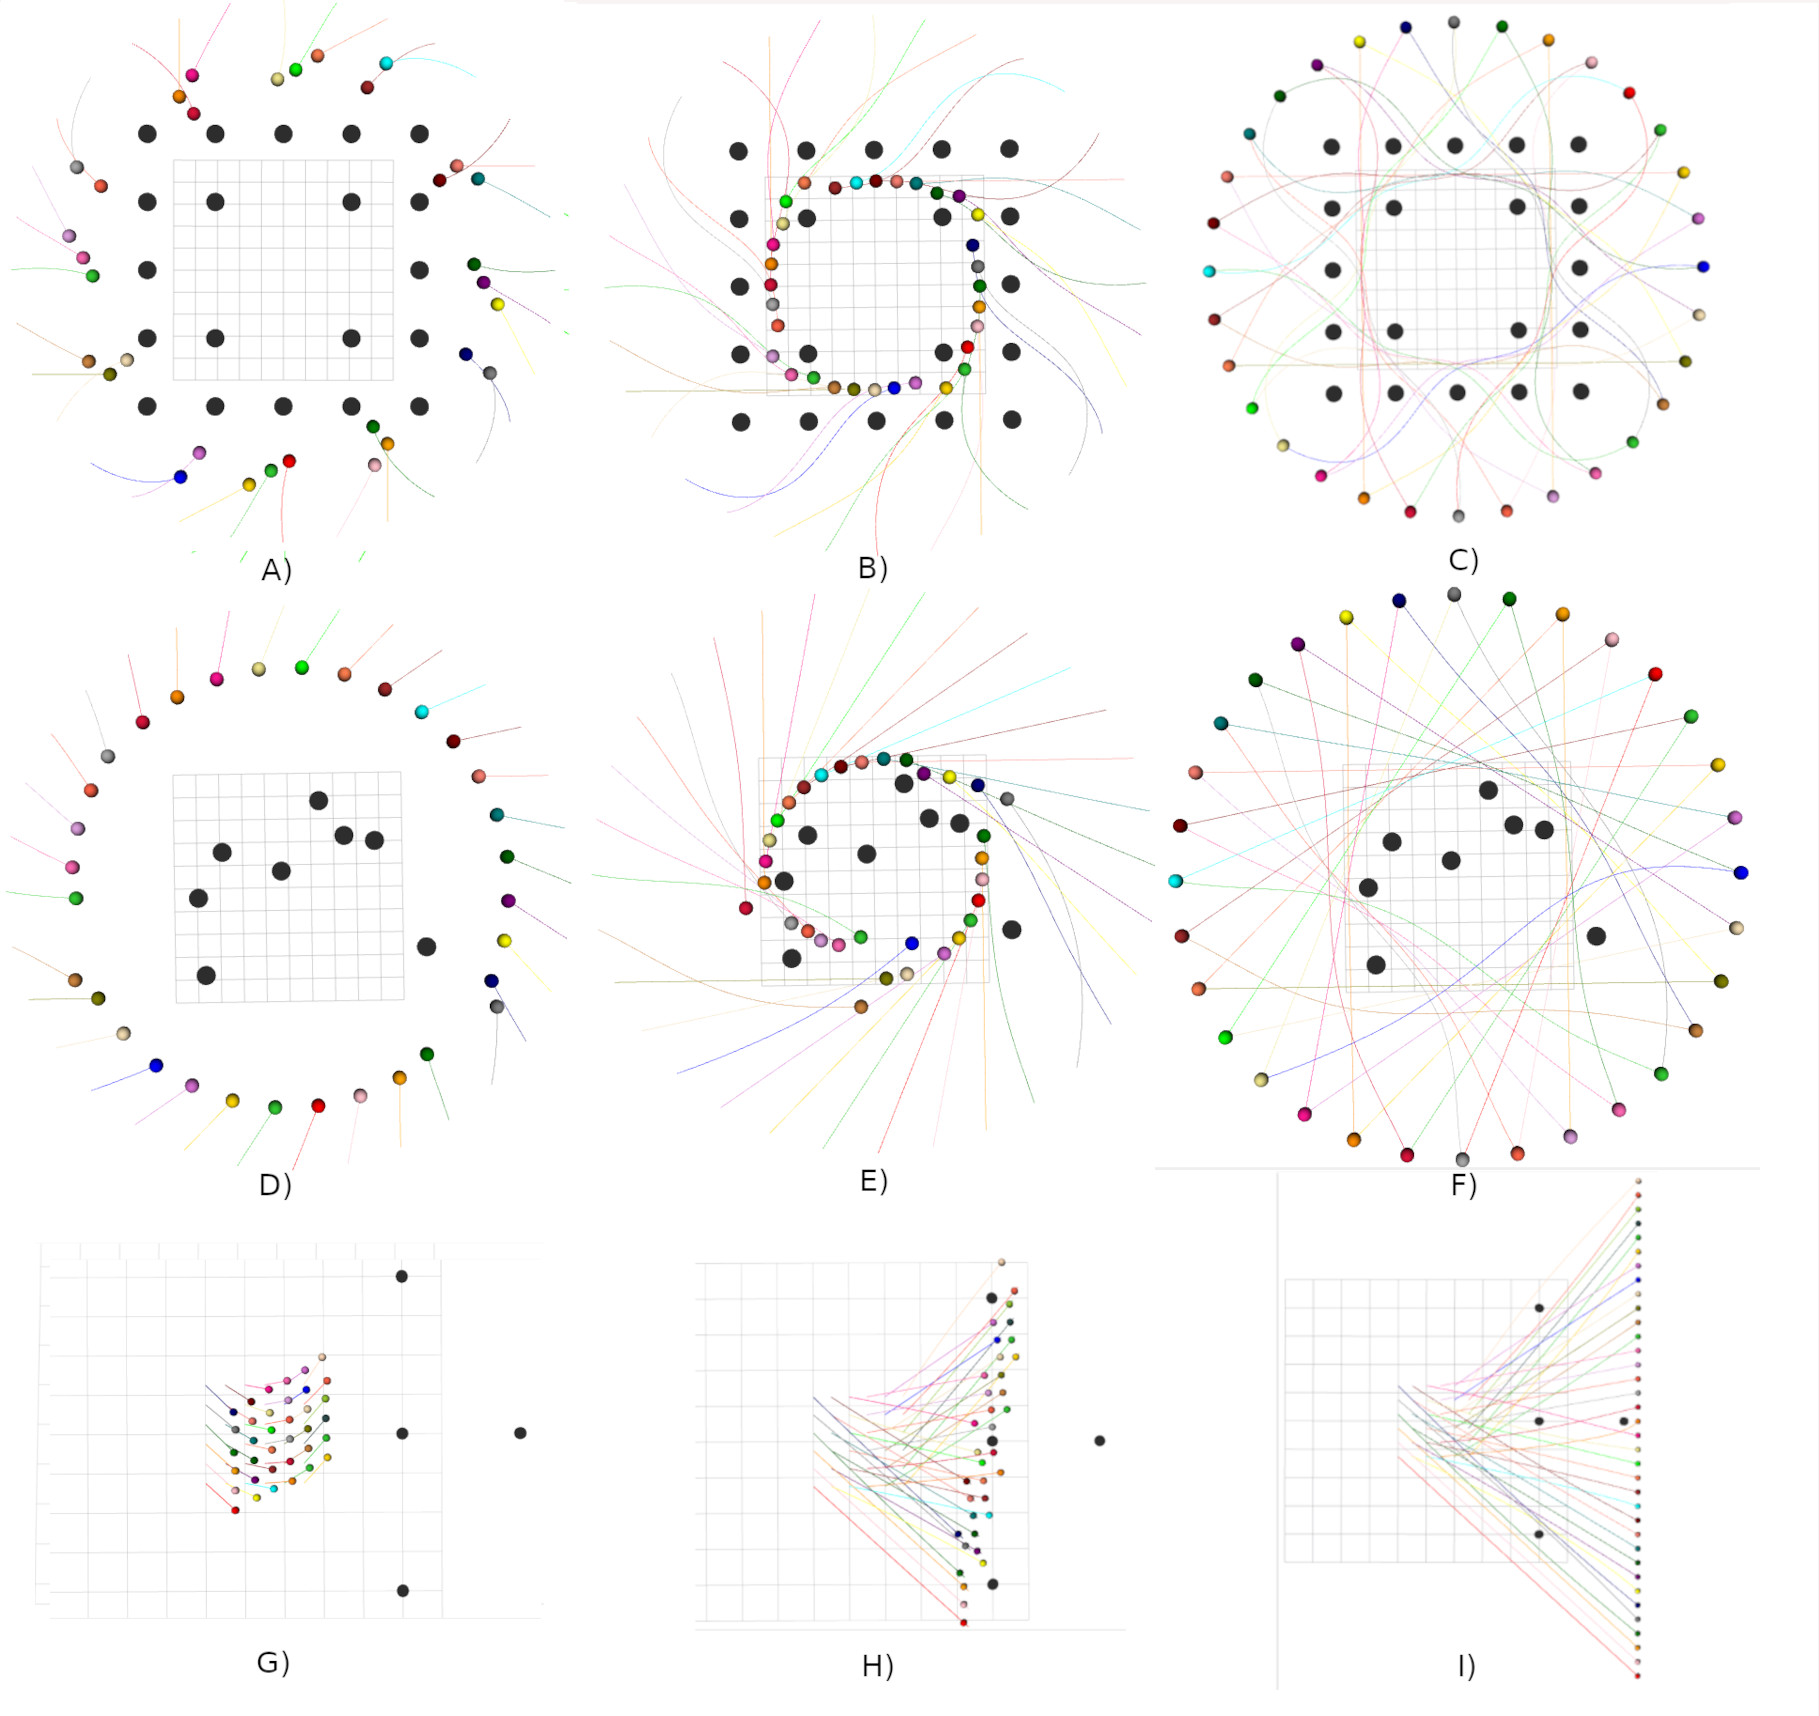
\includegraphics{figures/gpu_mat/trajectory_snapshots.jpg}} 
    \caption[Multi-robot Trajectory Snapshots]{Trajectory snapshots for (A-C) 32 robots, each of radius 0.3m arranged in a circle and 20 obstacles of radius 0.4m, (D-F) 32 robots, each of radius 0.3m arranged in a circle and 8 randomly placed obstacles of radius 0.4m, (G-I) 36 robots, each of radius 0.1m arranged in a grid configuration are required to move to a line formation. Also, the environment has 4 static obstacles, each of radius 0.15m.}
    \label{figure2}
\end{figure}

\begin{figure}
    \centering
    {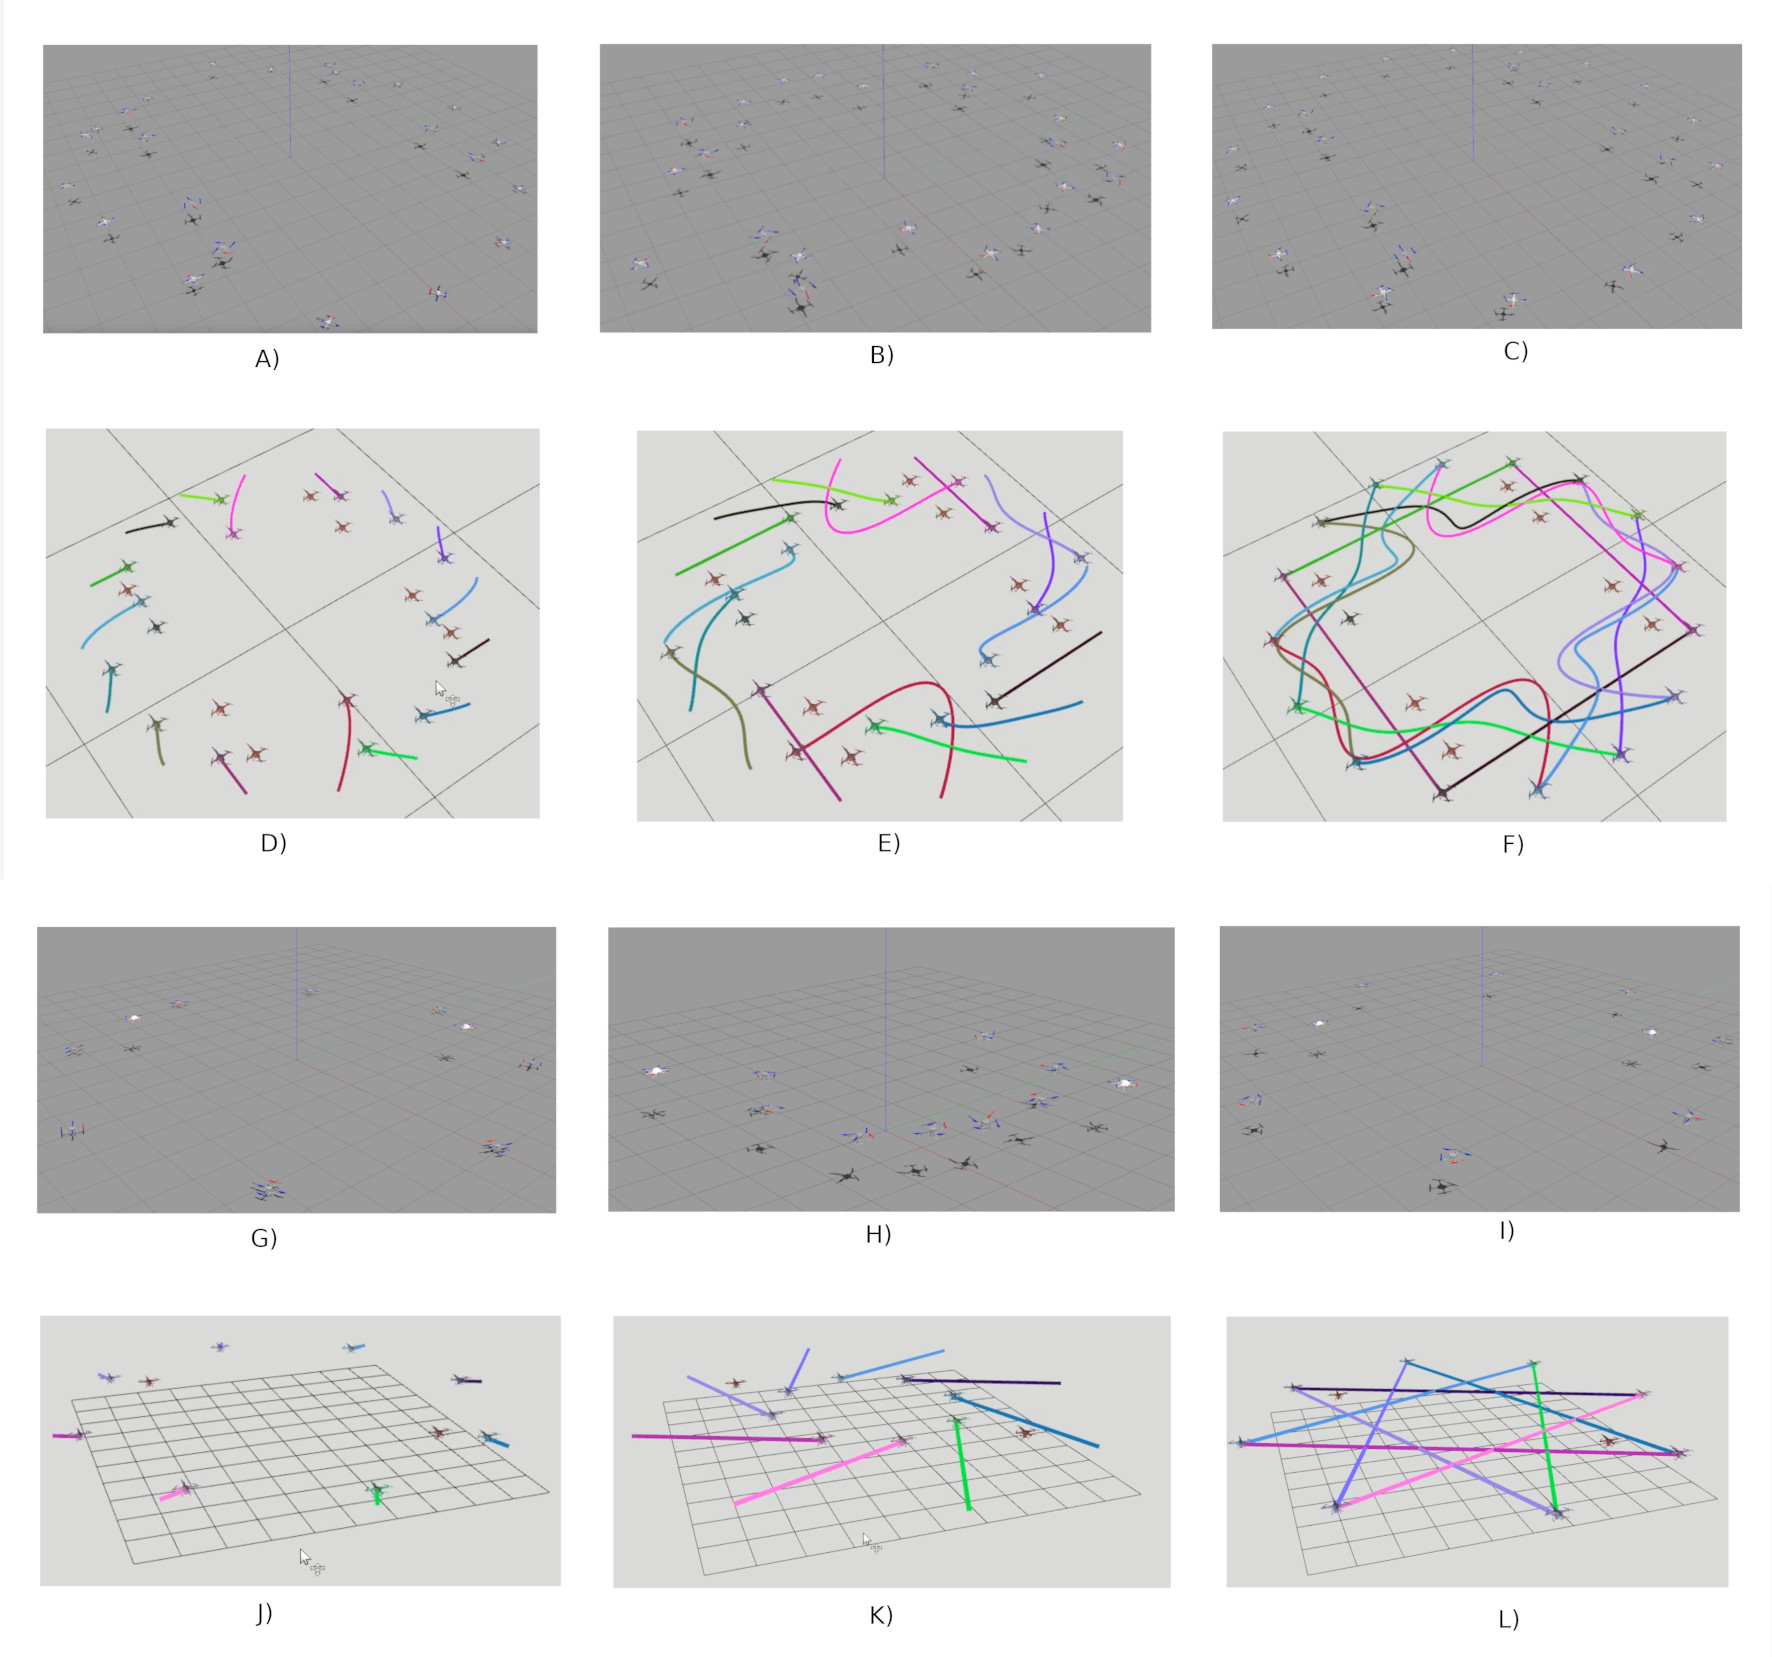
\includegraphics{figures/gpu_mat/gazebo_sim_snaps.jpg}} 
    \caption[Gazebo Simulation Snapshots]{Simulation snapshots for (A-F) 16 drones and 8 static obstacles of radius 0.3m, and (G-L) 8 drones and 2 static obstacles of radius 0.3m. (A-C) and (G-I) are screenshots of simulations on Gazebo. In (A-C), the gray static hovering drones represent static obstacles while in (G-I) white hovering drones represent static obstacles. (D-F) and (J-L) are screenshots of RViz simulations with the brown hovering drones representing static obstacles. For the full simulation videos, please refer to the following link: \url{https://www.dropbox.com/scl/fo/xnostapkvf72uudyb840t/h?dl=0&rlkey=02gjjllohbomzi0kcifbqezt9} }
    \label{figure_gazebo}
\end{figure}


A conceptually simple way of validating the convergence of the proposed optimizer is to observe the trends in residual of constraints \eqref{non_convex_equality_matrix-form} over iterations. If the residuals converge to zero, the computed trajectories are guaranteed to be collision-free. Fig. \ref{figure4} empirically provides this validation. It presents $\Vert \textbf{F}\boldsymbol{\xi}_{1, i}-\textbf{g}_i\Vert$ averaged over all $i$. Furthermore, we average the residuals over different trials in various benchmarks. We can observe from Fig.\ref{figure4} that, on average, 100 iterations are sufficient to obtain residuals around 0.01. A further increase in residuals can be obtained by increasing the number of iterations but at the expense of increasing the computation time. In our implementation, we adopt a heuristic wherein we inflate the size of the robots with four times the typical residual observed after 100 iterations.



\begin{figure}
    \centering
    {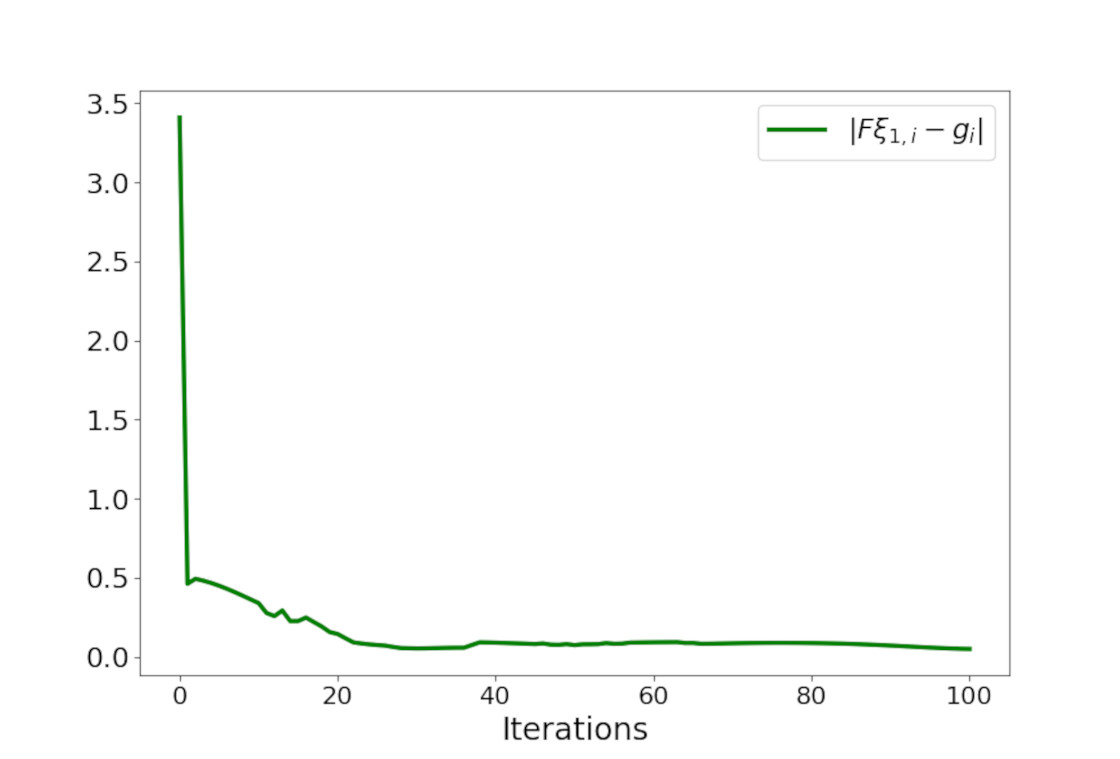
\includegraphics{figures/gpu_mat/cost_plots.jpg}} 
    \caption[GPU Optimizer Cost Plot]{Empirical validation of convergence of our optimizer. The figure shows the residual of $\Vert \textbf{F}\boldsymbol{\xi}_{1, i}-\textbf{g}_i\Vert$ averaged over all $i$ (agent index) and across different benchmarks.}
    \label{figure4}
\end{figure}

For a further sanity check, we check for inter-robot and robot-obstacle distances at each point along the computed trajectories (Fig. \ref{figure5}). Collisions are considered to have happened if the distances are less than sum of the robots' (blue line in Fig.\ref{figure5}) or robot-obstacles' (yellow line in Fig.\ref{figure5}) radii. Fig \ref{figure5} summarizes the average behavior observed across several trials, which validates the satisfaction of the collision avoidance requirement.


% shows the minimum pairwise distance between the centers of robots and obstacles for the scenarios considered in Fig \ref{figure2}. We observe that the minimum distance between any two robots always remains more than the sum of their radius, thereby guaranteeing no collision among robots. 


\begin{figure}
    \centering
    {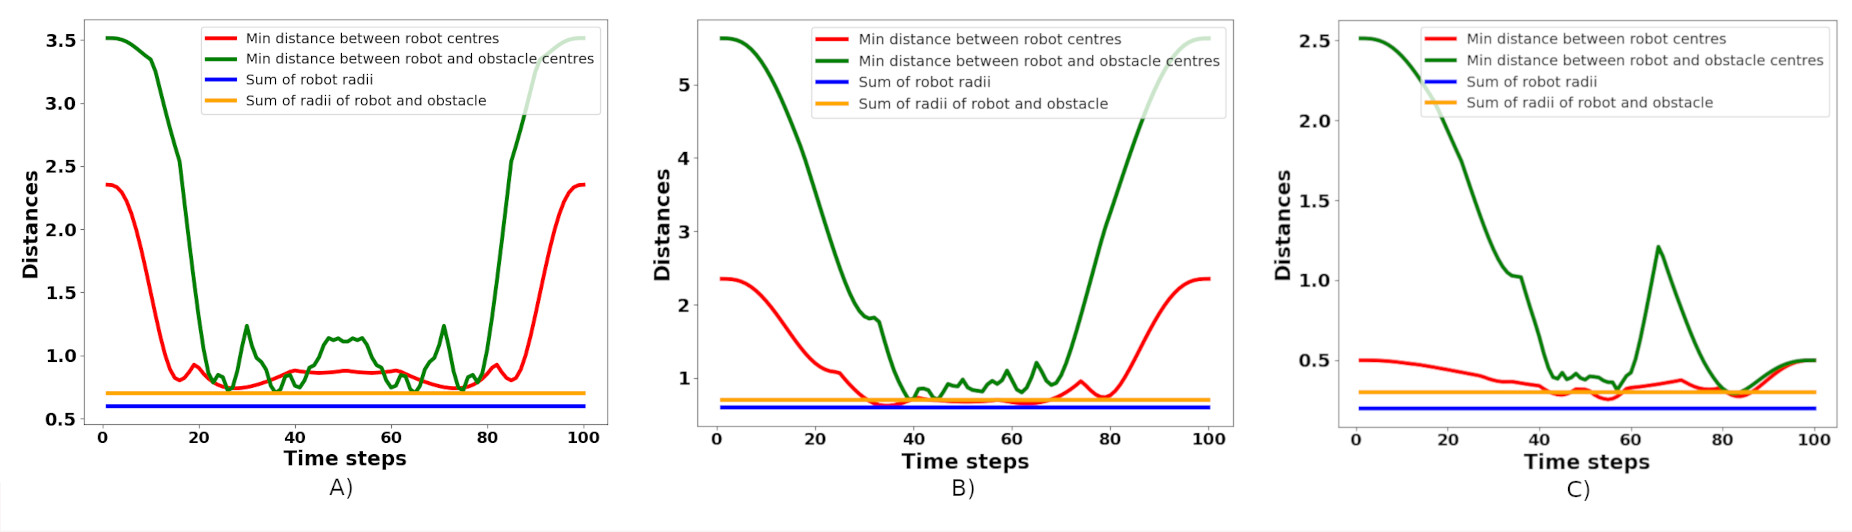
\includegraphics{figures/gpu_mat/min_distances.jpg}} 
    \caption[Minimum pairwise distances in benchmark scenes]{Figure showing the minimum of the pair-wise distances between the robots averaged across different benchmarks, some of which are shown in Fig.\ref{figure2}. The pair-wise distance is always greater than the lower bound shown in blue. Similarly, we also show the average minimum distance between the robots' and obstacles' centers. The corresponding lower bound is shown in yellow which is always respected by the computed trajectories.}
    \label{figure5}
\end{figure}


\subsection{Comparisons With State-of-the-Art}

\noindent This subsection compares our optimizer with existing state-of-the-art approaches \citep{aks_ral21} and \citep{park2020efficient}. We use the metrics Smoothness Cost, Arc-Length and Computation Time as discussed in Section \ref{sec:traj_eval_metrics}.


\subsubsection{Comparison with \citep{park2020efficient}}
Fig. \ref{figure6} presents a qualitative comparison between the trajectories obtained by our optimizer and \citep{park2020efficient} in two different benchmarks. Both approaches are successful; however, ours results in shorter trajectories. This trend is further confirmed by Fig.\ref{figure7}. Our optimizer achieves an average reduction of $3.90\%$ and $13.72\%$ in arc-length in 16 and 32 robots benchmarks, respectively. Furthermore, the performance gap between our optimizer and \citep{park2020efficient} increases as the environment becomes more cluttered with static obstacles. We also observe similar trends in the smoothness metric, with the performance gap being even starker. Our optimizer achieves an average reduction of $35.86\%$ and $59.06\%$ in smoothness cost in 16 and 32 robots benchmark, respectively.


Table \ref{table_comptime_seq} compares the computation time of our optimizer and \citep{park2020efficient}. Our optimizer shows better scaling with the number of robots and obstacles in the environment. On the considered benchmark, our optimizer shows a worst and best case improvement of $74.28 \%$ and $98.48 \%$ respectively. The trends in computation time can be understood in the following manner. The approach of \citep{park2020efficient} uses sampling-based multi-agent pathfinding algorithms to compute initial guesses for the robot trajectories. As the environment becomes more cluttered, the computational cost of computing the initial trajectories increases dramatically. Moreover, their sequential optimization also becomes increasingly more computationally intensive as the number of robots and obstacle increase. 

In contrast, our optimizer only requires matrix-matrix products, and the dimension of these matrices increases linearly with the number of robots and obstacles. This linear scaling along with GPU parallelization explains our computation time. 

\begin{figure}
    \centering
    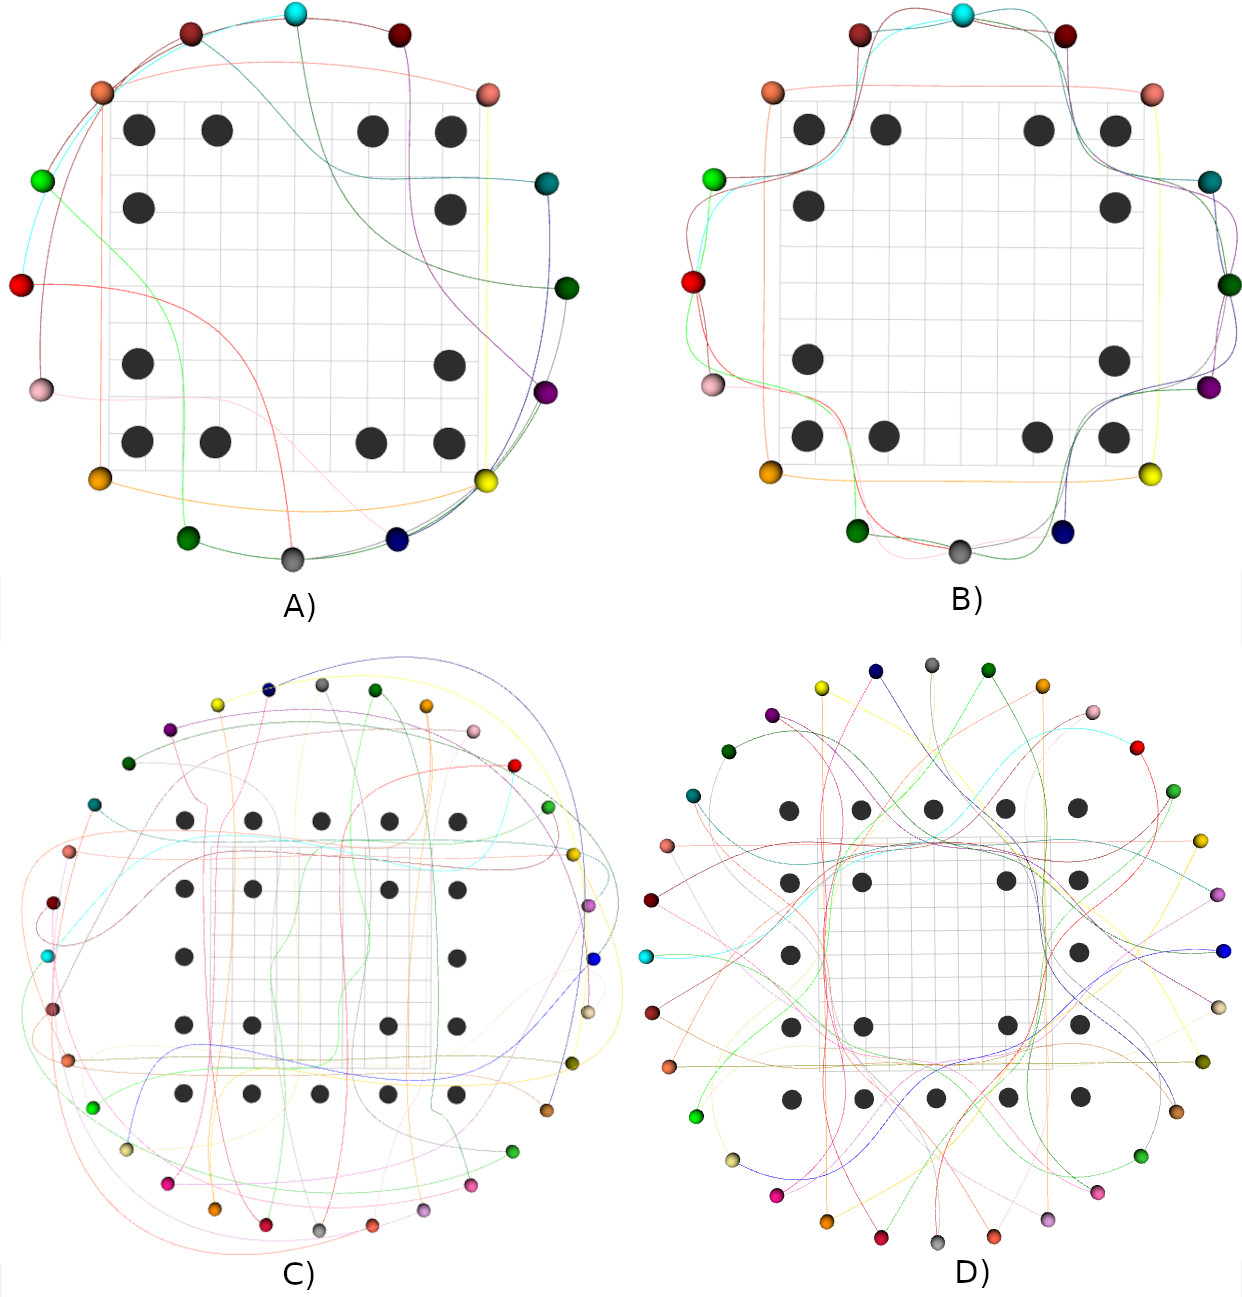
\includegraphics{figures/gpu_mat/qualitative_benchmark.jpg}
    \caption[Qualitative Benchmark against Multi-Robot State-of-the-Art]{Comparison of trajectories generated by \citep{park2020efficient}(A),C)) and our optimizer(B),D)) for 16 robots-12 obstacles (upper row) and 32 robots-20 obstacles (bottom row) benchmarks. Black spheres denote static obstacles and colored spheres denote robots. Our optimizer generates trajectories with smaller arc-length than \citep{park2020efficient}.}
    \label{figure6}
\end{figure}


\begin{figure}
    \centering
    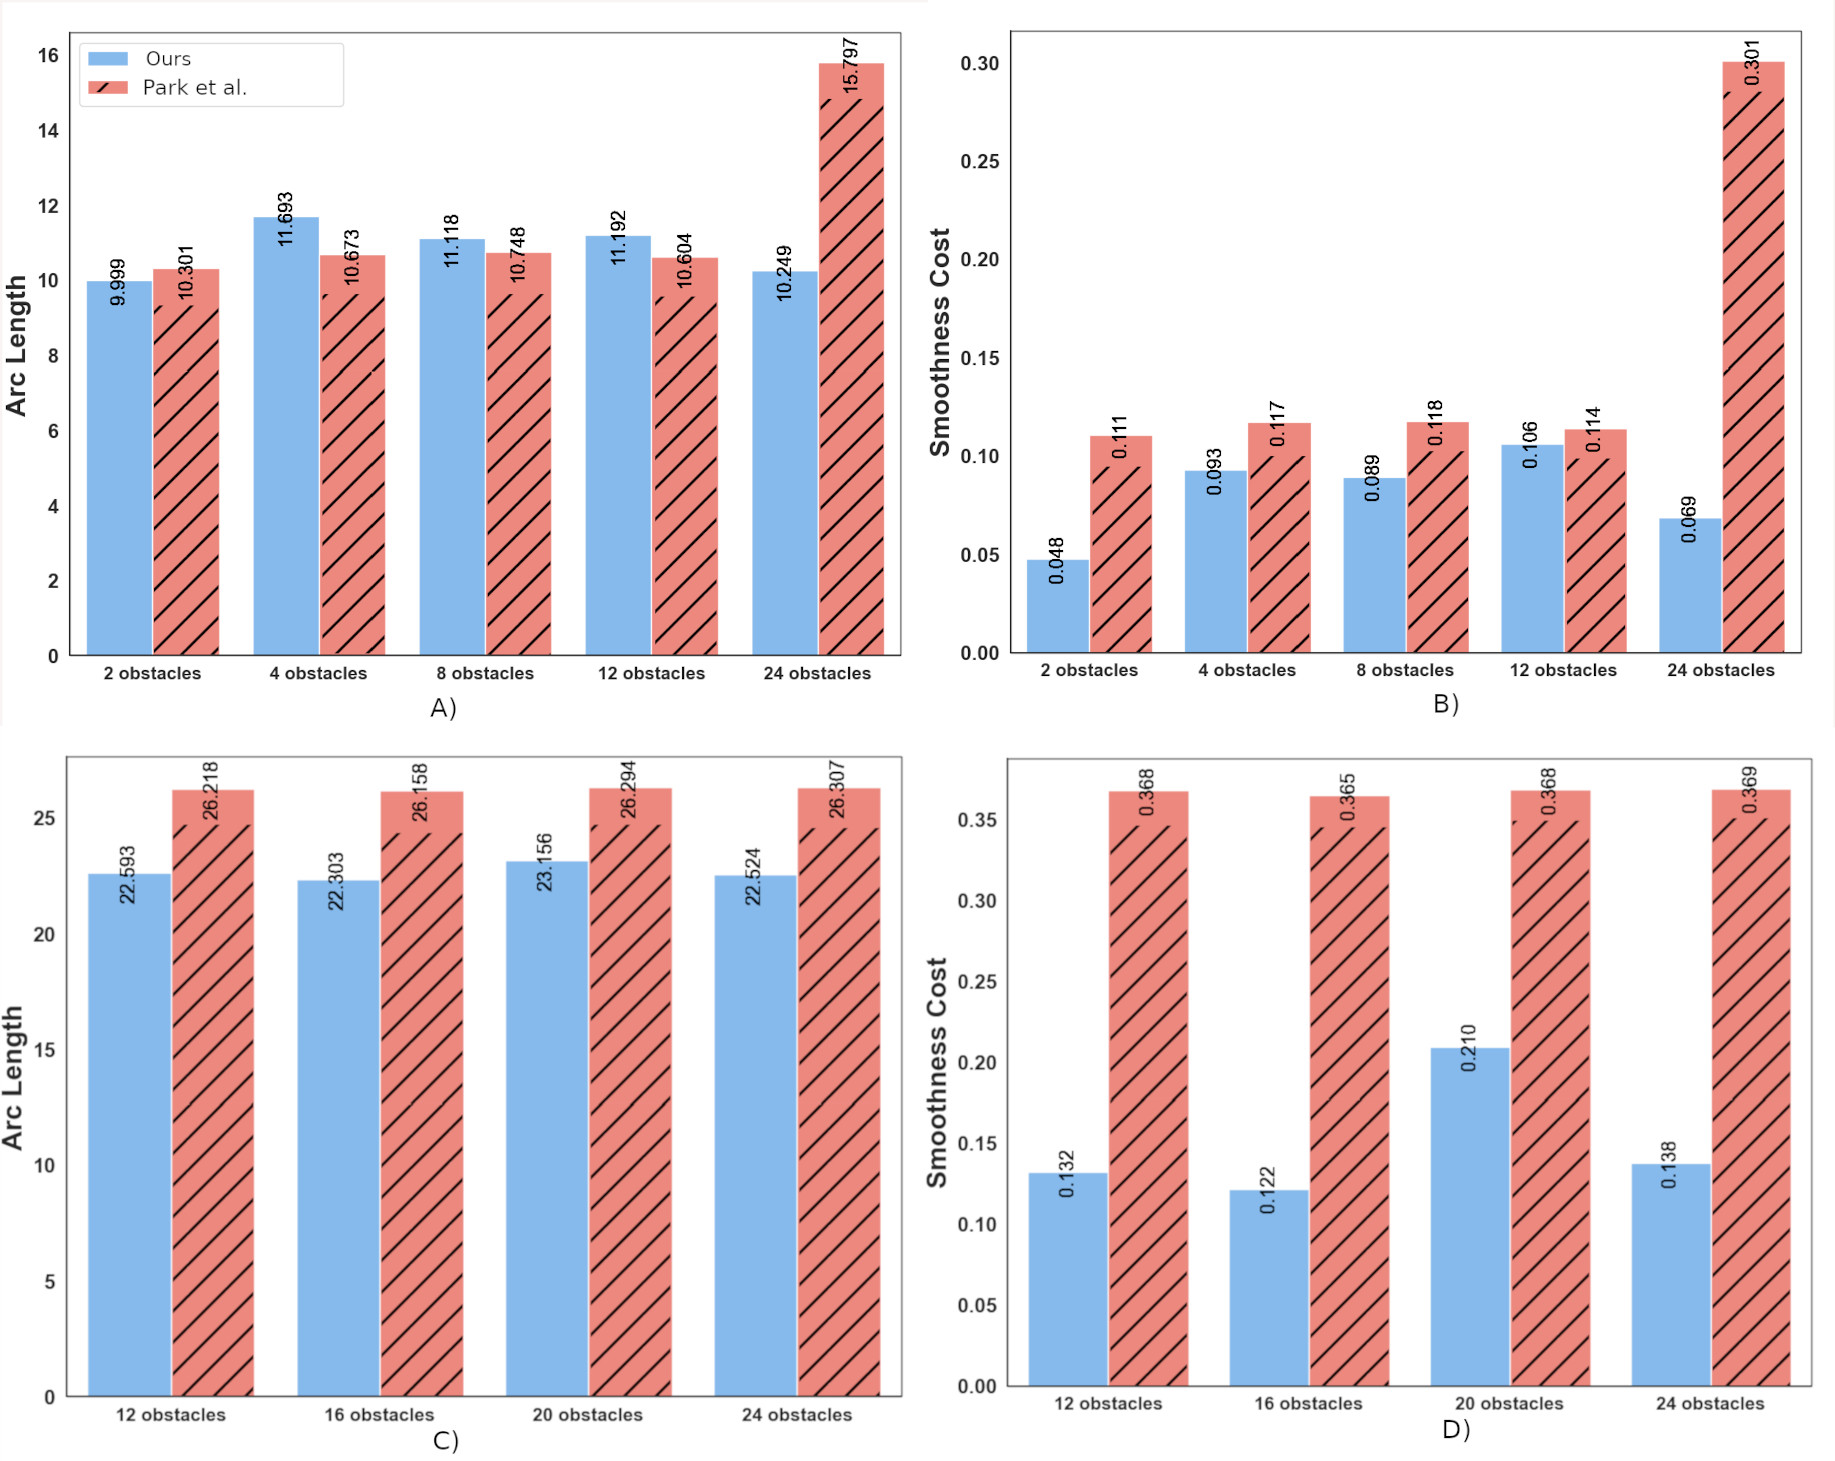
\includegraphics{figures/gpu_mat/quantitative_benchmark.jpg}
    \caption[Quantitative Benchmark against Multi-Robot State-of-the-Art]{Comparison of our optimizer with \citep{park2020efficient} in terms of arc-length and smoothness of obtained trajectories in 16 robots (A,B) and 32 robots (C,D) benchmarks. Our optimizer generates trajectories with not only better smoothness, but also with shorter arc-lengths. Moreover, the performance gap between our approach and \citep{park2020efficient} increases as the environment becomes more cluttered.}
    \label{figure7}
\end{figure}


\subsubsection{Comparison with \citep{aks_ral21}}
Table. \ref{table_3} compares the performance of our optimizer with \citep{aks_ral21}. Our core difference with \citep{aks_ral21} stems from the fact that we break a large optimization problem into smaller distributed sub-problems. In contrast, \citep{aks_ral21} retains the original larger problem itself. However, both our optimizer and  \citep{aks_ral21} use GPUs to accelerate the underlying numerical computations. Thus, unsurprisingly, \citep{aks_ral21} shows a decent scaling with the number of robots and obstacles. Nevertheless, our approach still outperforms \citep{aks_ral21}. Specifically, in 16 robot benchmarks, our optimizer shows a worst-case improvement of 2 times over \citep{aks_ral21} in computation time. As the environment becomes more cluttered, this factor increases to almost 10. In 32 robot benchmarks, the difference between our optimizer and \citep{aks_ral21}'s computation time is around nine times.

In terms of the arc-length and the smoothness metrics, our optimizer shows an improvement of around $57 \%$ and $58\%$ respectively over \citep{aks_ral21}. However, both approaches provide comparable results in the more challenging 32 robot benchmarks. The arc-length and smoothness cost difference decreases as the environment becomes more cluttered. 


\section{Ablation Study}

\subsection{Initializations using Reciprocal Velocity Obstacle(RVO)\cite{RVO}}\label{sec:appendix-RVO}

RVO is a local, reactive multi-robot trajectory planner that has been shown to generate collision-free trajectories in real-time for hundreds of robots\cite{RVO}. Even though it runs in real-time, RVO trajectories cannot be directly executed by Robots as they are jittery and jerky. We use a trick to precompute trajectories using RVO for given start and goal positions of multiple Robots and use the RVO trajectories along with other optimizer parameters computed from them to initialize our optimizer. Thus the task of eliminating collisions is first performed by RVO and further enhanced by our optimizer. We consider the velocity along the straight line joining the start and goal positions of the Robots as the desired velocity in RVO and sample the RVO trajectory obtained at evenly spaced intervals to match the number of time samples expected by the optimizer. We define the following set of additional configurations to test our optimizer with different types of initializations:

\begin{itemize}
  \item \textbf{Square Antipodal:}
  Robots are placed on the edge of a square and are needed to reach their antipodal positions. This scenario is particularly challenging since if the robots were moving in straight lines between the start and goal positions, they would all collide together at the center of the workspace.
  \item \textbf{Circle:}
  Robots are distributed evenly along a circle and are needed to rotate by $k$ positions. (default $k=5$).
  \item \textbf{Ellipse:}
  Robots are placed uniformly along a straight line, and the $i^{th}$ robot is needed to reach the position of the $(n-i)^{th}$ robot where $n$ is the total number of robots.
\end{itemize}

Figure \ref{fig:RVO+opti_2D} shows the trajectories generated by RVO alone for 16 Robots in the Square Antipodal scenario vs trajectories generated by our optimizer with RVO initialization. We observe a significant improvement in the smoothness of the trajectories generated by our optimizer with RVO initialization compared to RVO alone. The improvement in trajectory quality can be explained as follows: the optimizer starts with an already low residual due to RVO initialization and further reduces it with iterations while smoothing the trajectories at the same time. However, in terms of computation time, the RVO initialization does not offer significant benefits compared to a straight-line initialization of trajectories. 

\begin{figure}[H]
    \centering
    {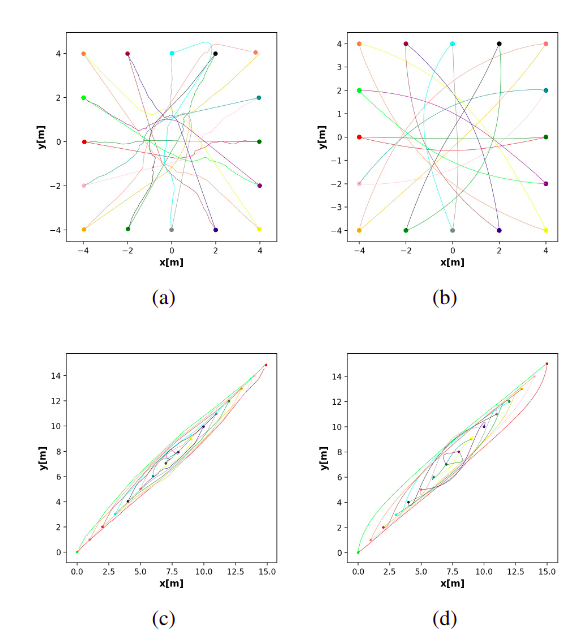
\includegraphics[scale=0.6]{figures/appendix/RVO_inits.png}} 
    \caption[Appendix: Trajectories using RVO + multi-robot optimizer]{Comparison of trajectories from a) RVO alone in 16 Robots 2D Square Antipodal b) Optimizer + RVO initialization for 16 Robots 2D Square Antipodal c) RVO alone in 16 Robots 2D Ellipse b) Optimizer + RVO initialization for 16 Robots 2D Ellipse.}
    \label{fig:RVO+opti_2D}
\end{figure}

\subsection{Initializations using Multi-robot Pathfinding(MAPF)\cite{sharon_journal}}\label{sec:appendix-MAPF}

Similar to RVO, we can also couple graph-search-based Multi-robot Pathfinding (MAPF) algorithms discussed in Section \ref{sec:MAPF} for initializing our optimizer. For this purpose, we will use the \texttt{cbs-mapf} PyPI package that implements the high-level Conflict Based Search Algorithm based on \cite{sharon_journal} and low-level space-time A*(STA*), which is similar to normal A*(from Section \ref{sec:A*} with an additional time dimension. The trajectories generated by CBS-MAPF are piecewise linear and exhibit jerks and sharp turns, so these cannot be used practically for multi-robot navigation. We scale up the start and goal coordinates depending on grid size (we use grid size = 10) as well as the robot radii and precompute multi-robot trajectories using CBS-MAPF. Similar to the RVO trajectories, we sample points from the trajectories obtained from CBS-MAPF to calculate the optimizer parameters and initialize our optimizer. 

We introduce a new scenario to test MAPF for 14 Robots arranged in a 2D grid and are needed to move to the opposite end of the grid. Figure \ref{fig:MAPF+opti_grid} shows a comparison of trajectories between CBS-MAPF alone and the optimizer using CBS-MAPF for initialization. We again observe a significant improvement in the smoothness of the trajectories generated by our optimizer with CBS-MAPF initialization compared to CBS-MAPF alone. However, similar to RVO, there is no benefit to using MAPF initialization in terms of computational time. 

\begin{figure}[H]
    \centering
    {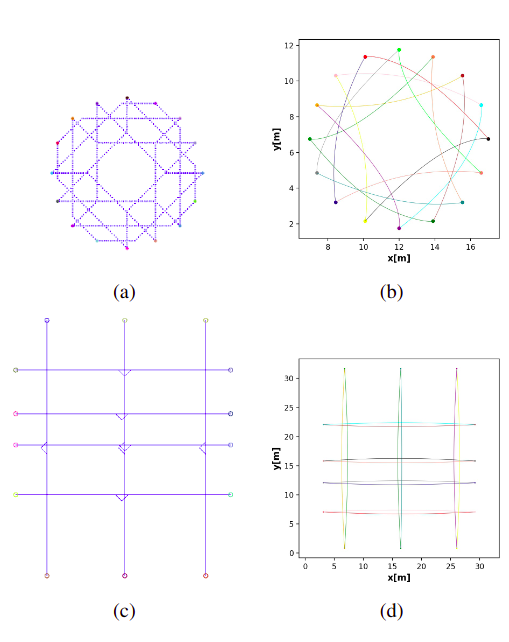
\includegraphics[scale=0.6]{figures/appendix/mapf_init.png}} 
    \caption[Appendix: Trajectories using MAPF + multi-robot optimizer]{Comparison of trajectories generated by CBS-MAPF alone and our optimizer with CBS-MAPF initialization for a)-b) 16 Robots in the Circle(k=5) scenario, c)-d) 14 Robots in 2D Grid orientation.}
    \label{fig:MAPF+opti_grid}
\end{figure}

\section{Discussions}

Joint multi-robot trajectory optimizations are generally considered intractable beyond a small number of robots. This is because the number of pair-wise collision avoidance constraints increases exponentially with the number of robots. Moreover, even the best optimization (QP) solvers show polynomial scaling with the number of constraints. We have fundamentally altered this notion through the discussion in this chapter. By employing a clever set of reformulations and parallelism offered by modern computing devices such as GPUs, we managed to compute trajectories for tens of robots in highly cluttered environments in a fraction of a second. Our formulation is simple to implement and involves computing just matrix-matrix products. Such computations can be trivially accelerated or parallelized on GPUs using off-the-shelf libraries like JAX (\cite{bradbury2020jax}). We benchmarked our approach against two strong state-of-the-art baselines and showed substantial improvement over them in terms of computation time and trajectory quality. 

Our work has potential beyond multi-robot coordination for interaction-aware trajectory prediction. We show in Sections \ref{sec:appendix-RVO} and \ref{sec:appendix-MAPF} how our multiagent optimizer may be used to improve the quality of trajectories obtained from multi-agent collision avoidance methods, such as Reciprocal Velocity Obstacle(RVO)\cite{RVO} and Multi-Agent Pathfinding(MAPF)\cite{sharon_journal}. 

It must be noted here that we were able to approximate collision constraints and solve the multi-robot path planning problem through gradient-based optimization due to the simplicity of the kinematics governing the motion of each robot. In this case, all the robots in the multi-robot system were holonomic. However, to extend this framework for car-like vehicles (non-holonomic robots), we would have to obey more complicated kinematic equations as discussed in Section \ref{sec:nonhn_robots}. When the robot kinematics becomes as complex as for manipulators, discussed in Section \ref{sec:bg-manipulator-kinematics}, even solving the trajectory optimization problem for a single robot may become intractable using gradient-based optimizers. This raises the need for a stochastic optimizer for robots with high-dimensional articulation, such as manipulators. In the next chapter, we will discuss how stochastic optimization can be used to generate collision-free trajectories for manipulators, and how the optimization can be decoupled into a bi-level framework, consisting of a global path planner and low-level motion planner.


%add some stuff about multiagent

%%%%%%%%%%%%%%%putting 1 line empty

\begin{table}
\centering
\caption{Important Symbols used in our optimizer} \label{table_1}
\scriptsize
\begin{tabular}{|p{3cm}|p{7cm}|p{7cm}|}\hline
\mbox{$n_{p}$, $n_{v}$, $n_{r}$}  & Planning steps, number of variables parameterizing trajectory along each motion axis, and number of robots, respectively.
\\ \hline
\mbox{ $a, b $} & Spheroid dimensions
\\ \hline
\mbox{$x_i(t), y_i(t), z_i(t)$} & 
 Position of $i^{th}$ robot at time $t$.
\\ \hline
\mbox{$\overline{x}_i(t), \overline{y}_i(t), \overline{z}_i(t)$} & Predicted position of $j^{th}$ agent.
\\ \hline
\mbox{$\boldsymbol{\lambda}_{i}$}
 &  Lagrangian multiplier 
\\ \hline
\end{tabular}
\normalsize
\vspace{-0.1cm}
\end{table}


%%%%%%%%%%%%%%%%%%%%%%one line empty

%%%%%%%%%%%%%%%%%%%% one line empty 

\begin{table}
\begin{center}
\caption{Comparison with current state-of-the-art \citep{park2020efficient} in terms of computation time.  }
\label{table_comptime_seq}
\begin{tabular}{ |p{3.5cm}|p{3cm}|p{2cm}|p{2cm}|}
\hline
 Number of robots & Number of Obstacles & ours[s] & \citep{park2020efficient}[s]  \\
 \hline
 32 & 24 & 0.21 &  12.897\\
 \hline
 32 & 20 &  0.20 &  11.827\\
 \hline
 32 & 16 & 0.20 & 12.423\\
 \hline
 32 & 12 & 0.19 & 12.504\\
 \hline
 16 & 24 & 0.17 & 0.795\\ 
 \hline
 16 & 12 & 0.17& 0.661\\
 \hline
 16 & 8 & 0.16& 0.680\\
 \hline
 16 & 4 & 0.16 & 0.702\\
 \hline
 16 & 2 & 0.15 & 0.621\\
 \hline
\end{tabular}
\end{center}
\end{table}

%%%%%%%%%%%%%%%%%%%%%%%%%%%%%%%%%%%%%%%%%%%%
%%%%%%%%%%%%%%%%%%%%%%%% one line empty 

\begin{table}
\centering
\caption{ Comparison with \citep{aks_ral21} in terms of computation time, arc-length and smoothness cost }
\label{table_3}
\scriptsize
\begin{tabular}{|p{2cm}|p{2.5cm}|p{3.5cm}|p{2cm}|p{2cm}|p{2cm}|}
\hline
Number of robots & Number of Obstacles &Benchmark & Computation time[s] & Arc-length[M] & Smoothness cost  \\ 
\hline
 \multirow{2}{*}{}&2  & \citep{aks_ral21}  &  0.34 & 13.488 & 0.102\\  
 \cline{2-6} 
 \multirow{2}{*}{}&2  & Ours &  0.15  &  9.999 & 0.048\\  
 \cline{2-6}
 \multirow{2}{*}{16 robot}& 4 & \citep{aks_ral21} & 0.37 & 14.257& 0.114\\
 \cline{2-6}
  \multirow{2}{*}{}& 4 & Ours  & 0.16 & 11.693& 0.093\\
 \cline{2-6}
 \multirow{2}{*}{}&8 & \citep{aks_ral21} & 0.70 &15.539 & 0.140\\
 \cline{2-6}
  \multirow{2}{*}{}&8 & Ours & 0.16 &11.118 & 0.089\\
 \cline{2-6}
 \multirow{2}{*}{}&12 & \citep{aks_ral21}  & 0.79 & 15.931 & 0.159\\
  \cline{2-6}
\multirow{2}{*}{} & 12  & Ours & 0.17 & 11.192 & 0.106\\ 
\cline{2-6}
 \multirow{2}{*}{}&24 & \citep{aks_ral21}  &1.49  & 24.198 & 0.164\\
  \cline{2-6}
\multirow{2}{*}{} & 24  & Ours & 0.17 & 10.249 & 0.069\\ 
\hline \hline
\multirow{2}{*}{} & 12  & \citep{aks_ral21} & 1.688 & 23.855  &0.157\\
\cline{2-6}
\multirow{2}{*}{} & 12  & Ours & 0.19 & 22.593 & 0.132\\
\cline{2-6}
\multirow{2}{*}{} & 16  & \citep{aks_ral21} & 1.752 &24.04 &0.164\\
\cline{2-6}
\multirow{2}{*}{32 robots} & 16  & Ours & 0.20 & 22.303 &0.122 \\
\cline{2-6}
\multirow{2}{*}{} & 20 & \citep{aks_ral21} & 1.804  &24.14 &0.170\\
\cline{2-6}
\multirow{2}{*}{} & 20  & Ours & 0.20 & 23.156 &0.210 \\
\cline{2-6}
\hline
\end{tabular}
\normalsize
\end{table}

%%%%%%%%%%%%%%%%%%%%%one line empty

% \section{\label{sec:abstract}Abstract}

% Near-term quantum hardware can support two-qubit operations only on the qubits that can interact with each other. Therefore, to execute an arbitrary quantum circuit on the hardware, compilers have to first perform the task of qubit routing, i.e., to transform the quantum circuit either by inserting additional SWAP gates or by reversing existing CNOT gates to satisfy the connectivity constraints of the target topology.  The depth of the transformed quantum circuits is minimized by utilizing the Monte Carlo tree search (MCTS) to perform qubit routing by making it both construct each action and search over the space of all actions. It is aided in performing these tasks by a Graph neural network that evaluates the value function and action probabilities for each state. Along with this, we propose a new method of adding mutex-lock like variables in our state representation which helps factor in the parallelization of the scheduled operations, thereby pruning the depth of the output circuit. Overall, our procedure (referred to as QRoute) performs qubit routing in a hardware agnostic manner, and it outperforms other available qubit routing implementations on various circuit benchmarks.

% {\smaller (Published in the Proceedings of AAAI Conferenence on Artificial Intelligence, 2022 \cite{self-qroute})}    
% %\tableofcontents

% \section{\label{sec:intro}Introduction}

% The present-day quantum computers, more generally known as Noisy Intermediate-Scale quantum (NISQ) devices \cite{nisq_preskill} come in a variety of hardware architectures \cite{IBMQ, hardware_sycamore, hardware_rigetti_aspen, hardware_xanadu}, but there exist a few problems pervading across all of them. These problems constitute the poor quality of qubits, limited connectivity between qubits, and the absence of error-correction for noise-induced errors encountered during the execution of gate operations. These place a considerable restriction on the number of instructions that can be executed to perform useful quantum computation \cite{nisq_preskill}. Collectively these instructions can be realized as a sequential series of one or two-qubit gates that can be visualized more easily as a quantum circuit as shown in Fig. \ref{fig:orig_circ} \cite{others_childs}.

% To execute an arbitrarily given quantum circuit on the target quantum hardware, a compiler routine must transform it to satisfy the connectivity constraints of the topology of the hardware \cite{qroute_tket}. These transformations usually include the addition of SWAP gates and the reversal of existing CNOT gates. This ensures that any non-local quantum operations are performed only between the qubits that are nearest-neighbors. This process of circuit transformation by a compiler routine for the target hardware is known as qubit routing \cite{qroute_tket}. The output instructions in the transformed quantum circuit should follow the connectivity constraints and essentially result in the same overall unitary evolution as the original circuit \cite{qroute_dqn2}.

% In the context of NISQ hardware, this procedure is of extreme importance as the transformed circuit will, in general, have higher depth due to the insertion of extra SWAP gates. This overhead in the circuit depth becomes more prominent due to the high decoherence rates of the qubits and it becomes essential to find the most optimal and efficient strategy to minimize it \cite{qroute_tket, qroute_dqn1, qroute_dqn2}. In this chapter, we present a procedure that we refer to as \textit{QRoute}. We use Monte Carlo tree search (MCTS), which is a look-ahead search algorithm for finding optimal decisions in the decision space guided by a heuristic evaluation function \cite{mcts_bandit_1, mcts_bandit_2, mcts_uct}. We use it for explicitly searching the decision space for depth minimization and as a stable and performant machine learning setting. It is aided by a Graph neural network (GNN) \cite{nn_edge_conv}, with an architecture that is used to learn and evaluate the heuristic function that will help guide the MCTS.

% %\textit{Structure}: In Section \ref{sec:qubit-routing}, we introduce the problem of qubit routing, the previous works that are done in the field, and show how our work differs from them. The methodology of the QRoute algorithm is described in Section \ref{sec:method}. In Section \ref{sec:results}, we benchmark the performance of our algorithm against other state-of-the-art quantum compilers. Finally, we discuss our results and  possible improvements in Section \ref{sec:discussion-conclusion}.

% \begin{figure}
%     \centering
%     \hfill
%     \begin{subfigure}[b]{0.30\linewidth}
%         \includegraphics[width=\textwidth]{figures/qroute/orig_circ.pdf}
%         \caption{Quantum circuit\label{fig:orig_circ}}
%     \end{subfigure}
%     \hfill
%     \begin{subfigure}[b]{0.30\linewidth}
%         \includegraphics[width=0.85\textwidth]{figures/qroute/sliced_circ.pdf}
%         \caption{Decomposed circuit\label{fig:sliced_circ}}
%     \end{subfigure}
%     \hfill
%     \begin{subfigure}[b]{0.35\linewidth}
%         \includegraphics[width=\textwidth]{figures/qroute/transformed_circ.pdf}
%         \caption{Decomposed transformed circuit\label{fig:transformed_circ}}
%     \end{subfigure}
%     \hfill
%     \caption[Topologies of Quantum Computing hardware qRoute is tested on]{An example of qubit routing on a quantum circuit for 3$\times$3 grid architecture (Figure \ref{fig:3-3-arch}). (a) For simplicity, the original quantum circuit consists only of two-qubit gate operations. (b) Decomposition of the original quantum circuit into series of slices such that all the instructions present in a slice can be executed in parallel. The two-qubit gate operations: $\{d,e\}$ (green) comply with the topology of the grid architecture whereas the operations: $\{a, b, c, f\}$ (red) do not comply with the topology (and therefore cannot be performed). Note that the successive two-qubit gate operations on $q_3\rightarrow q_4$ (blue) are redundant and are not considered while routing. (c) Decomposition of the transformed quantum circuit we get after qubit routing. Four additional SWAP gates are added that increased the circuit depth to $5$, i.e., an overhead circuit depth of $2$. The final qubit labels are represented at the end right side of the circuit. The qubits that are not moved (or swapped) are shown in brown ($\{q_1, q_5\}$), while the rest of them are shown in blue.}
%     %Note that the overall unitary operation performed by the circuit is preserved despite the changes in the order of two-qubit gate operations.}
%     \label{fig:routing-example}
% \end{figure}

% \begin{figure}
%     \centering
%     \begin{subfigure}[b]{0.4\linewidth}
%         \centering
%         \includegraphics[width=0.5\linewidth]{figures/qroute/Grid-device.pdf}
%         \caption{3$\times$3 grid architecture with edges (i.e. neighboring qubits) labelled \label{fig:3-3-arch}}
%     \end{subfigure}
%     \begin{subfigure}[b]{0.5\linewidth}
%         \centering
%         \includegraphics[width=0.5\linewidth]{figures/qroute/QX20-device.pdf}
%         \caption{IBMQX-20 architecture represented as a graph}
%     \end{subfigure}
%     \caption{Examples of qubit connectivity graphs for some common quantum architectures}
%     \label{fig:topology-example}
% \end{figure}

% \section{\label{sec:qubit-routing}Qubit Routing}
% In this section, we begin by defining the problem of qubit routing formally and discussing the work done previously in the field.

% \subsection{\label{sec:intro-defn}Describing the Problem}
% The topology of quantum hardware can be visualized as a qubit connectivity graph (Fig. \ref{fig:topology-example}). Each node in this graph would correspond to a physical qubit which in turn might correspond to a logical qubit. The quantum instruction set, which is also referred to as quantum circuit (Fig. \ref{fig:orig_circ}), is a sequential series of single-qubit and two-qubit gate operations that act on the logical qubits. The two-qubit gates such as CNOT can only be performed between two logical qubits iff there exists an edge between the nodes that correspond to the physical qubits, \cite{qroute_dqn1}. This edge could be either unidirectional or bidirectional, i.e., CNOT can be performed either in one direction or in both directions. In this work, we consider only the bidirectional case, while noting that the direction of a CNOT gate can be reversed by sandwiching it between a pair of Hadamard gates acting on both control and target qubits \cite{utk_equiv_circuits}. 

% Given a target hardware topology $\mathcal{D}$ and a quantum circuit $\mathcal{C}$, the task of qubit routing refers to transforming this quantum circuit by adding a series of SWAP gates such that all its gate operations then satisfy the connectivity constraints of the target topology (Fig. \ref{fig:transformed_circ}). Formally, for a routing algorithm $\textrm{R}$, we can represent this process as follows:
% \begin{equation}
% \textrm{R}(\mathcal{C},\ \mathcal{D}) \rightarrow \mathcal{C}^{\prime}
% \end{equation}
% Depth of $\mathcal{C}^{\prime}$ (transformed quantum circuit) will, in general, be more than that of the original circuit due to the insertion of additional SWAP gates. This comes from the definition of the term \textit{depth} in the context of quantum circuits. This can be understood by decomposing a quantum circuit into series of individual slices, each of which contains a group of gate operations that have no overlapping qubits, i.e., all the instructions present in a slice can be executed in parallel (Fig. \ref{fig:sliced_circ}). The depth of the quantum circuit then refers to the minimum number of such slices the circuit can be decomposed into, i.e., the minimum amount of parallel executions needed to execute the circuit. The goal is to minimize the overhead depth of the transformed circuit with respect to the original circuit.

% This goal involves solving two subsequent problems of (i) qubit allocation, which refers to the mapping of program qubits to logic qubits, and (ii) qubit movement, which refers to routing qubits between different locations such that interaction can be made possible \cite{utk_qubit_noise}. In this work, we focus on the latter problem of qubit movement only and refer to it as qubit routing. However, it should be  noted that qubit allocation is also an important problem and it can play an important role in minimizing the effort needed to perform qubit movement.



% \subsection{\label{sec:intro-related}Related Work}

% The first major attraction for solving the qubit routing problem was the competition organized by IBM in 2018 to find the best routing algorithm. This competition was won by \cite{zulehner2018mapping}, for developing a Computer Aided Design-based (CAD) routing strategy. Since then, this problem has been presented in many different ways. These include graph-based architecture-agnostic solution by \cite{qroute_tket}, showing equivalence to the travelling salesman problem by \cite{paler_torus}, machine learning based methods by \cite{paler_ml}, and heuristic approaches by \cite{review-1}, \cite{review-2}, \cite{review-3}, etc. A reinforcement learning in a combinatorial action space solution was proposed by \cite{qroute_dqn1}, which suggested used simulated annealing to search through the combinatorial action space, aided by a Feed-Forward neural network to judge the long-term expected depth. This was further extended to use Double Deep Q-learning and prioritized experience replay by \cite{qroute_dqn2}. 

% Recently, Monte Carlo tree search (MCTS), a popular reinforcement learning algorithm \cite{mcts_survey} previously proven successful in a variety of domains like playing puzzle games such as Chess and Go \cite{mcts_alphago}, and was used by \cite{qroute_mcts} to develop a qubit routing solution. 
% %However, they used MCTS in the context of minimizing the total volume of quantum circuits (i.e., the number of gates ignoring the parallelization).

% % \begin{figure*}[t]
% %     \includegraphics[width=\linewidth]{figures/qroute/Evolution.pdf}
% % 	\caption{\label{fig:routing-progress}Routing progress for 3$\times$3 grid architecture while for the quantum circuit in Fig. \ref{fig:orig_circ}. Initial state shows the gate scheduled on each qubit which gets executed as control and target qubit adjacent to each other via SWAPs (shown in green and purple). The final state (at time=$5$) shows the final evolved qubit mapping. Here, each state (at time step=$t$) corresponds to the $t^{\rm{th}}$ time slice in Fig. \ref{fig:transformed_circ}}
% % \end{figure*}

% \subsection{\label{sec:intro-contribution}Our Contributions}

% Our work demonstrates the use of MCTS on the task of Qubit Routing and presents state of the art results. Following are the novelties of this approach:

% \begin{itemize}
%     \item We use an array of mutex locks to represent the current state of parallelization, helping to reduce the depth of the circuits instead of the total quantum volume, in contrast to previous use of MCTS for qubit routing in \cite{qroute_mcts}.
%     \item The actions in each timestep (layer of the output circuit) belong to a innumerably large action space. We phrase the construction of such actions as a Markov decision process, making the training stabler and the results better, particularly at larger circuit sizes, than those obtained by performing simulated annealing to search in such action spaces \cite{qroute_dqn1, qroute_dqn2}. Such approach should be applicable to other problems of a similar nature.
%     \item Graph neural networks are used as an improved architecture to help guide the tree search.
% \end{itemize}

% Finally, we provide a simple python package containing the implementation of QRoute, together with  an easy interface for trying out different neural net architectures, combining algorithms, reward structures, etc.

% \begin{figure}[ht]
%     \centering
%     \includegraphics[width=\linewidth]{figures/qroute/Search.pdf}
%     \caption[Visualization of steps in Monte Carlo Tree Search]{
%         Iteration of a Monte Carlo tree search: (i) select - recursively choosing a node in the search tree for exploration using a selection criteria, (ii) expand - expanding the tree using the available actions if an unexplored leaf node is selected, (iii) rollout - estimating long term reward using a neural network for the action-state pair for the new node added to search tree, and (iv) backup - propagating reward value from the leaf nodes upwards to update the evaluations of its ancestors.}
%     \label{fig:mcts-explainer}
% \end{figure}


% \newtheorem{defn}{Definition}[section]

% \section{\label{sec:method}Method}

% The QRoute algorithm takes in an input circuit and an injective map, $\mathcal{M}: Q \rightarrow N$, from logical qubits to nodes (physical qubits). Iteratively, over multiple timesteps, it tries to schedule the gate operations that are present in the input circuit onto the target hardware. To do so, from the set of unscheduled gate operations, $\mathcal{P}$, it takes all the current operations, which are the first unscheduled operation for both the qubits that they act on, and tries to make them into local operations, which are those two-qubit operations that involve qubits that are mapped to nodes connected on the target hardware.

% In every timestep $t$, QRoute starts by greedily scheduling all the operations that are both current and local in $\mathcal{P}$. To evolve $\mathcal{M}$, it then performs a Monte Carlo tree search (MCTS) to find an optimal set of SWAPs by the evaluation metrics described in the Section \ref{sec:method-mcts} such that all operations in the current timestep put together form a parallelizable set, i.e., a set of local operations such that no two operations in the set act on the same qubit. The number of states we can encounter in the action space explodes exponentially with the depth of our search, therefore an explicit search till the circuit is done compiling is not possible. Therefore we cut short our search at some shallow intermediate state, and use a neural network to get its heuristic evaluation. Detailed algorithm has been presented in appendix \ref{appendix:mcts}.


% The following subsections describe in greater detail the working of the search and the heuristic evaluation.

% \subsection{\label{sec:method-state} State and Action Space}

% \begin{defn}[State]
%     It captures entire specification of the state of compilation at some timestep t. Abstractly, it is described as:
%     \begin{equation}
%         s_{t} = (\mathcal{D}, \ \mathcal{M}_{t},\ \mathcal{P}_{t},\ \mathcal{L}_{t})
%     \end{equation}

%     where, $\mathcal{D}$ is the topology of target hardware, and $\mathcal{M}_t$ and $\mathcal{P}_t$ represents the current values of $\mathcal{M}$ and $\mathcal{P}$ respectively. $\mathcal{L}_{t}$ is the set of nodes that are locked by the gate operations from the previous timestep and therefore cannot be operated in the current timestep. 
% \end{defn}


% \begin{defn}[Action]
%     It is a set of SWAP gates (represented by the pair of qubits it acts on) such that all gates are local, and its union with the set of operations that were scheduled in the same timestep forms a parallelizable set.
% \end{defn}

% We are performing a tree search over state-action pairs. Since the number of actions that can be taken at any timestep is exponential in the number of connections on the hardware, we are forced to build a single action up, step-by-step. 

% \begin{defn}[Move]
%     It is a single step in a search procedure which either builds up the action or applies it to the current state. Moves are of the following two types:
%     \begin{enumerate}
%         \item SWAP($n_1$, $n_2$): Inserts a new SWAP on nodes $n_1$ and $n_2$ into the action set. Such an insertion is only possible if the operation is local and resulting set of operations for the timestep form a parallel set.
%         \item COMMIT: Finishes the construction of the action set for that timestep. It also uses the action formed until now to update the state $s_t$ (schedules the SWAP gates on the hardware), and resets the action set for the next step.
%     \end{enumerate}
% \end{defn}

% In reality, different gate operations take different counts of timesteps for execution. For example, if a hardware requires SWAP gate to be broken down into CNOT gates, then it would take three timesteps for complete execution \cite{utk_equiv_circuits}. This means, operations which are being scheduled must maintain mutual exclusivity with other other operations over the nodes which participates in them. This is essential to minimizing the depth of the circuit since it models paralleizability of operations.

% However, constructing a parallelizable set and representing the state of parallelization to our heuristic evaluator is a challenge. But an analogy can be drawn here to the nodes being thought of as ``resources" that cannot be shared, and the operations as ``consumers" \cite{mutex_dijkstra}. This motivates us to propose the use of Mutex Locks for this purpose. These will lock a node until a scheduled gate operation involving that node executes completely. Therefore, this allows our framework to naturally handle different types of operations which take different amounts of time to complete.

% % On some hardware, SWAP gates are not primitive and get decomposed to three CNOT gates. Therefore they are thrice as slow as other primitive gates. This is easily modelled by keeping the mutex locks for those nodes locked for three timesteps. Therefore, this allows our framework to naturally handle different types of operations which take different amounts of time to complete.

% For every state-action pair, the application of a feasible move $m$ on it will result in a new state-action pair: $(s,a) \xrightarrow[]{m} (s^\prime,a^\prime)$. This is a formulation of the problem of search as a Markov Decision Process. Associated with each such state-action-move tuple $((s, a), m)$, we maintain two additional values that are used by MCTS:

% \begin{enumerate}
% \item \textit{N-value} - The number of times we have taken the said move $m$ from said state-action pair $(s,a)$.
% \item \textit{Q-value} - Given a reward function $\mathcal{R}$, it is the average long-term reward expected after taking said move $m$ over all iterations of the search. (Future rewards are discounted by a factor $\gamma$)

% \begin{equation}
% \begin{split}
%     Q((s,a), m) =&\ \mathcal{R}((s,a), m)\ + \\ & \gamma \frac{\sum_{m^\prime} N((s^\prime, a^\prime), m^\prime) \cdot Q((s^\prime, a^\prime), m^\prime)}{\sum_{m^\prime} N((s^\prime, a^\prime), m^\prime)}
% \end{split}
% \end{equation}

% \end{enumerate}

% \begin{figure*}[th]
% \centering
%     \includegraphics[width=\textwidth]{figures/qroute/Architecture.pdf}
%     \caption[Graph neural network architecture that approximates value and policy function]{\label{fig:network-architecture}
%      Graph neural network architecture that approximates the value function and the policy function.}
%      %The $state$ object (orange), shown on the far left, is provided as an input. The edge convolution block (yellow) extracts the features from the input object, collects them, flattens them, and concatenates them with the rest of the input for further processing. Here, the network diverges into two segments, one called the value head, which gives a scalar output representing the quality of the state, and another policy head, which provides the probability distribution over the best action from this state.}
% \end{figure*}

% \subsection{\label{sec:method-mcts} Monte Carlo Tree Search}

% Monte Carlo tree search progresses iteratively by executing its four phases: select, expand, rollout, and backup as illustrated in Fig. \ref{fig:mcts-explainer}. In each iteration, it begins traversing down the existing search tree by selecting the node with the maximum UCT value (Eq. \ref{eq:uct}) at each level. During this traversal, whenever it encounters a leaf node, it expands the tree by choosing a move $m$ from that leaf node. Then, it estimates the scalar evaluation for the new state-action pair and backpropagates it up the tree to update evaluations of its ancestors.

% To build an optimal action set, we would want to select the move $m$ with the maximum true Q-value. But since true Q-values are intractably expensive to compute, we can only approximate the Q-values through efficient exploration. We use the Upper Confidence Bound on Trees (UCT) objective \cite{mcts_uct} to balance exploration and exploitation as we traverse through the search tree. Moreover, as this problem results in a highly asymmetric tree, since some move block a lot of other moves, while others block fewer moves, we use the formulation of UCT adapted for asymmetric trees \cite{mcts_assymetric}:

% \begin{equation}\label{eq:uct}
% \begin{split}
%     \textrm{UCT}((s,a), m) =&\ Q((s,a), m)\ + \\ & c \frac{\sqrt{\sum_m N((s,a), m)}}{N((s,a), m)} \times p(m \vert (s,a))
% \end{split}
% \end{equation}

% Here, the value $p(m | (s,a))$ is the prior policy function, which is obtained by adding a Dirichlet noise to the policy output of the neural network \cite{mcts_alphazero}. As MCTS continues probing the action space, it gets a better estimate of the true values of the actions. This means that it acts as a policy enhancement function whose output policy (Eq. \ref{eq:mcts_output}) can be used to train the neural network's prior ($\pi$), and the average Q-value computed can be used to train its scalar evaluation (Eq. \ref{eq:train_nn}).

% \begin{equation}\label{eq:mcts_output}
%     \pi(m | (s,a)) \propto N((s, a), m))
% \end{equation}

% \begin{equation}\label{eq:train_nn}
%     \mathcal{V}((s,a)) = \frac{\sum_{m} Q((s,a), m)}{\sum_{m} N((s,a), m)}
% \end{equation}



% The details of how MCTS progresses have been elaborated in the supplementary. Once it gets terminated, i.e., the search gets completed, we go down the tree selecting the child with the maximum Q-value at each step until a COMMIT action is found, we use the action set of the selected state-action pair to schedule SWAPs for the current timestep, and we re-root the tree at the child node of the COMMIT action to prepare for the next timestep.

% \subsection{\label{sec:method-model}Neural Network Architecture}

% Each iteration of the MCTS requires evaluation of Q-values for a newly encountered state-action pair. But these values are impossible to be computed exactly since it would involve an intractable number of iterations in exploring and expanding the complete search tree. Therefore, it is favorable to heuristically evaluate the expected long-term reward from the state-action pair using a Neural Network, as it acts as an excellent function approximator that can learn the symmetries and general rules inherent to the system.

% So, once the MCTS sends a state-action pair to the evaluator, it begins by committing the action to the state and getting the resultant state. We then generate the following featurized representation of this state and pass this representation through the neural-network architecture as shown in Fig. \ref{fig:network-architecture}.

% \begin{enumerate}
%     \item \textit{Node Targets} - It is a square boolean matrix whose rows and columns correspond to the nodes on a target device. An element $(i, j)$ is true iff some logical qubits $q_x$ and $q_y$ are currently mapped to nodes $i$ and $j$ respectively, such that ($q_x$, $q_y$) is the first unscheduled operation that $q_x$ partakes in.
%     \item \textit{Locked Edges} - It is a set of edges (pairs of connected nodes) that are still locked due to either of its qubits being involved in an operation in the current timestep or another longer operation that hasn't yet terminated from the previous timesteps.
%     \item \textit{Remaining targets} - It is a list of the number of gate-operations that are yet to be scheduled for each logical qubit. 
% \end{enumerate}

% % \begin{enumerate}
% %     \item The \textbf{target node} for some node $n_1$ is a node $n_2$, such that if qubit $q_1$ is currently mapped to $n_1$ and $q_2$ is mapped to $n_2$, then the operation ($q_1$, $q_2$) is the first operation in the input circuit that $q_1$ partakes in, which has not already been scheduled.
% %     \item The number of \textbf{remaining targets} for some qubit $q$ is the number of operations involving it which are yet to be scheduled.
% %     \item \textbf{Locked edges} is the set of edges (pairs of connected qubits) which are still locked due to either of it's qubits being involved in an operation in the current timestep or a longer operation that hasn't yet terminated from the previous timestep.
% % \end{enumerate}

% The SWAP operations each qubit would partake in depends primarily on its target node, and on those of the nodes in its neighborhood that might be competing for the same resources. It seems reasonable that we can use a Graph Neural Network with the device topology graph for its connectivity since the decision of the optimal SWAP action for some node is largely affected by other nodes in its physical neighborhood. Therefore, our architecture includes an edge-convolution block \cite{nn_edge_conv}, followed by some fully-connected layers with Swish \cite{nn_swish} activations for the policy and value heads. The value function and the policy function computed from this neural network are returned back to the MCTS.



% \section{\label{sec:results}Results}
% We compare QRoute against the routing algorithms from other state-of-the-art frameworks on various circuit benchmarks: (i) Qiskit and its three variants \cite{comp_qiskit}: (a) basic, (b) stochastic, and (c) sabre, (ii) Deep-Q-Networks (DQN) from \cite{qroute_dqn2}, (iii) Cirq \cite{comp_cirq}, and (iv) t$\ket{\text{ket}}$ from Cambridge Quantum Computing (CQC) \cite{comp_pytket}. 
% % The routing algorithm in t$\ket{\text{ket}}$ uses BRIDGE gates along with SWAP gates and
% Qiskit's transpiler uses gate commutation rules while perform qubit routing. This strategy is shown to be advantageous in achieving lower circuit depths \cite{bridge_gate} but was disabled in our simulations to have a fair comparison. The results for DQN shown are adapted from the data provided by the authors \cite{qroute_dqn2}. Additional data regarding performance on Google Sycamore, the specific results on each circuit, etc., have been provided in the appendix \ref{appendix:mcts}.

% \begin{figure}[t]
%     \includegraphics[width=\linewidth]{figures/qroute/random_benchmark.pdf}
%     \caption[qRoute Results on randomly generated circuits]{\label{fig:results-random}
%         Comparative performance of routing algorithms on random circuits as a function of the number of two-qubit operations in the circuit.}
% \end{figure}

% \subsection{\label{sec:results-random}Random Test Circuits}

% The first benchmark for comparing our performance comprises of random circuits. These circuits are generated on the fly and initialized with the same number of qubits as there are nodes on the device. Then two-qubit gates are put between any pair of qubits chosen at random. In our simulations, the number of such gates is varied from 30 to 150 and the results for assessing performance of different frameworks are given in Fig. \ref{fig:results-random}. The experiments were repeated 10 times on each circuit size, and final results were aggregated over this repetition. 


% Amongst the frameworks compared, QRoute ranks a very close second only to Deep-Q-Network guided simulated annealer (DQN). Nevertheless, QRoute still does consistently better than all the other major frameworks: Qiskit, Cirq and t$\ket{\text{ket}}$, and it scales well when we increase the number of layers and the layer density in the input circuit. QRoute shows equivalent performance to DQN on smaller circuits, and on the larger circuits it outputs depths which are on average $\leq 4$ layers more than those of DQN. Some part of this can be attributed to MCTS, in its limited depth search, choosing the worse of two moves with very close Q-values, resulting in the scheduling of some unnecessary SWAP operations.


% \subsection{\label{sec:results-small}Small Realistic Circuits}

% Next we test on the set of all circuits which use 100 or less gates from the IBM-Q realistic quantum circuit dataset used by \cite{data_realistic}. The comparative performance of all routing frameworks has been shown by plotting the depths of the output circuits summed over all the circuits in the test set in Fig. \ref{fig:results-small}. Since the lack of a good initial qubit allocation becomes a significant problem for all pure routing algorithms on small circuits, we have benchmarked QRoute on this dataset from three trials with different initial allocations.

% The model presented herein has the best performance on this dataset. We also compare the best result from a pool of all routers including QRoute against that of another pool of the same routers but excluding QRoute. The pool including QRoute gives on average $2.5\%$ lower circuit depth, indicating that there is a significant number of circuits where QRoute is the best routing method available.

% \begin{figure}[t]
%     \includegraphics[width=\linewidth]{figures/qroute/realistic_small_benchmark.pdf}
%     \caption[qRoute Results on small realistic circuit set]{\label{fig:results-small}
%         Plots of output circuit depths of routing algorithms over small realistic circuits ($\leq 100$ gates), summed over the entire dataset. The inset shows the results on the same data comparing the best performant scheduler excluding and including QRoute on each circuit respectively.}
% \end{figure}



% \begin{figure*}[ht]
%     \centering
%     \includegraphics[width=\linewidth]{figures/qroute/realistic_large_benchmark.pdf}
%     \caption[qRoute Results on large realistic circuit set]{\label{fig:results-large}
%         The results over eight circuits sampled from the large realistic dataset benchmark, the outputs of each routing algorithm are shown for every circuit.}
% \end{figure*}

% On this dataset also, closest to QRoute performance is shown by Deep-Q-Network guided simulated annealer. To compare performances, we look at the average circuit depth ratio (CDR), which is defined by \cite{qroute_dqn2}:
% \begin{equation}
%     \text{CDR} = \frac{1}{\textrm{\#circuits}} \sum_{\textrm{circuits}} \frac{\textrm{Output Circuit Depth}}{\textrm{Input Circuit Depth}}
%     \label{eq:CDR}
% \end{equation}
% The resultant CDR for QRoute is $1.178$, where as the reported CDR for the DQN is $1.19$. In fact, QRoute outperforms DQN on at least $80\%$ of the circuits. This is significant because in contrast to the random circuit benchmark, the realistic benchmarks consist of the circuits that are closer to the circuits used in useful computation.


% \subsection{\label{sec:results-realistic}Large Realistic Circuit}

% For final benchmark, we take eight large circuits ranging from 154 gates to 5960 gates in its input from the IBM-Quantum realistic test dataset \cite{data_realistic}. The results are plotted in Fig.  \ref{fig:results-large}. QRoute has the best performance of all available routing methods: Qiskit and t$\ket{\text{ket}}$, on every one of these sampled circuits with on an average $13.6\%$ lower circuit depth, and notable increase in winning difference on the larger circuits.



% The results from DQN and Cirq are not available for these benchmarks as they are not designed to scale to such huge circuits. In case of DQN, the CDR data results were not provided for the circuits over $200$ gates, mainly because simulated annealing used in it is computationally expensive. Similarly, for Cirq, it takes several days to compile each of the near $5000$ qubit circuits. In contrast, QRoute is able to compile these circuits in at most 4 hours, and its compilation process can be sped up by reducing the depth of the search. Spending more time, however, helps MCTS to better approximate the Q-values leading to circuits with lower resulting depth.



% \section{\label{sec:discussion-conclusion}Discussion and Conclusion}
% %I'm writing this vaguely. Improve upon stuff wherever possible and let's meet at night. 

% In this chapter, we have shown that the problem of qubit routing has a very powerful and elegant formulation in Reinforcement Learning (RL) which can surpass the results of any classical heuristic algorithm across all sizes of circuits and types of architectures. Furthermore, the central idea of building up solutions step-by-step when searching in combinatorial action spaces and enforcing constraints using mutex locks, can be adapted for several other combinatorial optimization problems \cite{comb_survey, comb_1, comb_2, comb_3, comb_4}. Our approach is flexible enough to compile circuits of any size onto any device, from small ones like IBMQX20 with 20 qubits, to much larger hardware like Google Sycamore (results provided in supplementary) with 53 qubits (the Circuit Depth Ratio for small realistic circuits on Google Sycamore was 1.64). Also, it intrinsically deals with hardware having different primitive instruction set, for example on hardware where SWAP gates are not a primitive and they get decomposed to 3 operations. QRoute enjoys significant tunability; hyperparameters can be changed easily to alter the tradeoff between time taken and optimality of decisions, exploration and exploitation, etc.

% QRoute is a reasonably fast method, taking well under 10 minutes to route a circuit with under 100 operations, and at most 4 hours for those with upto 5000 operations, when tested on a personal machine with an i3 processor (3.7 GHz) and no GPU acceleration. Yet more can be desired in terms of speed. However, it is hard to achieve any significant improvement without reducing the number of search iterations and trading off a bit of performance. More predictive neural networks can help squeeze in better speeds.

% One of the challenges of methods like DQN, that use Simulated Annealing to build up their actions is that the algorithm cannot plan for the gates which are not yet waiting to be scheduled, those which will come to the head of the list once the gates which are currently waiting are executed \cite{qroute_dqn2}. QRoute also shares this deficiency, but the effect of this issue is mitigated by the explicit tree search which takes into account the rewards that will be accrued in the longer-term future. There is scope to further improve this by feeding the entire list of future targets directly into our neural network by using transformer encoders to handle the arbitrary length sequence data. This and other aspects of neural network design will be a primary facet of future explorations. Another means of improving the performance  would be to introduce new actions by incorporating use of BRIDGE gates \cite{bridge_gate} and gate commutation rules \cite{utk_equiv_circuits} alongside currently used SWAP gates. The advantage of former is that it allows running CNOT gates on non-adjacent qubit without permuting the ordering of the logical qubits; whereas, the latter would allow MCTS to recognize the redundancy in action space, making its exploration and selection more efficient.

% Finally, we provide an open-sourced access to our software library. It will allow researchers and developers to implement variants of our methods with minimal effort. We hope that this will aid future research in quantum circuit transformations. For review we are providing, the codebase and a multimedia in the supplementary.  

% On the whole, the Monte Carlo Tree Search for building up solutions in combinatorial action spaces has exceeded the current state of art methods that perform qubit routing. Despite its success, we note that QRoute is a primitive implementation of our ideas, and there is great scope of improvement in future. 


%--------------------------------------------------------

\chapter{Stochastic Trajectory Optimization for Robot Manipulators}
\label{ch:bl_arm}
\section{\label{qleet-sec:abstract}Abstract}

Manipulating a target object using a fixed-base robot manipulator presents a complex problem that requires addressing multiple constraints, such as optimizing the manipulator joint cost, finding a collision-free trajectory, and modeling the object dynamics. Previous approaches have relied on contact-rich manipulation, where the object moves predictably while attached to the manipulator, thereby avoiding the need to model the object's dynamics, which does not generalize to multiple types of end-effectors. Further, collision avoidance for manipulators in existing approaches rely on context-specific neural network-based object representation, which need to be retrained for each specific arrangement and type of obstacles and robots.  
We first discuss a stochastic trajectory optimizer, Via-point Stochastic Trajectory Optimization and adapt it for context-agnostic path planning in the joint space for commonly-used robot manipulators, such as the Franka Panda and UR5e. Next, we propose a novel framework that disentangles the non-prehensile long-horizon manipulation problem into planning and control. The planning component uses the aforementioned context-agnostic Via-Point stochastic trajectory optimizer, generating a collision-free trajectory from the start to the goal position, consisting of multiple via-points. This simplifies the task of the reinforcement learning based control component, which only needs to move the object closer to the next via-point. We pair the high-level via-point planner with a low-level push controller based on Deep Reinforcement Learning, that is gripper-agnostic. A key contribution of our approach is that the planning module predicts the most optimal path for the control component given the scene context using a bi-level optimization scheme. Our experimental results demonstrate that the proposed framework can generalize to arbitrary scenes with multiple collision objects of different shapes and sizes. We evaluate the framework on a few complex scenes using a two-fingered gripper and show improvements over different related approaches.

\section{Introduction}

Object manipulation is an essential task for robots to perform that has many diverse downstream applications, for example in the service industry (manipulating kitchenware~\cite{kitchen_arm}), industrial setting (packaging~\cite{industrial_arm}) and household (tabletop rearrangement~\cite{agarwal2022approaches}). Broadly, object manipulation can be of two types - \textit{Prehensile}, which involves continuous contact-rich gripping of the object using the manipulator's end-effector(gripper or a hand-like structure), and \textit{Non-Prehensile}, which involves moving the object without grasping it. Prehensile actions are often used in manufacturing, packaging, and assembly processes where the robot needs to handle and manipulate objects of various shapes and sizes. On the other hand, non-prehensile actions are typically used when the object is too fragile or too large to be picked up by the robot's gripper. Instead, the robot uses other methods such as pushing, pulling, sliding, or rolling to move the object around. Non-prehensile manipulator actions are commonly used in applications such as warehouse automation, sorting, and material handling.

Path planning for manipulators involves finding a collision-free path for a robot arm or manipulator to follow as it moves from its current position to a desired position. Any trajectory sent to a manipulator to be followed must satisfy the dynamic and kinematic constraints of the robot, as well as the workspace bounds in which it operators. A few commonly-used approaches to path planning for manipulators include the following:

\begin{itemize}
    \item \textit{Sampling-based Methods:} These methods randomly sample the configuration space of the robot (i.e., the set of all possible positions and orientations) and attempt to find a collision-free path by connecting the samples together. Examples of sampling-based methods include Rapidly-exploring Random Trees(RRTs)\cite{RRT-og} and Probabilistic Roadmaps (PRMs)\cite{PRM}.
    \item \textit{Search-based Methods:} These methods search for a path through the configuration space using a search algorithm, such as A*\cite{A*} or Dijkstra's algorithm. Search-based methods can be combined with heuristics to reduce the search space and improve performance.
    \item \textit{Optimization-based Methods:} These methods formulate the path planning problem as an optimization problem, where the objective is to find the shortest path that satisfies certain constraints (e.g., collision avoidance). Optimization may be performed by gradient-based updates or by sampling potential candidates from a distribution and updating the distribution itself after evaluating the cost of the candidates. 

\end{itemize}

In this chapter, we will explore optimization-based methods for path planning for manipulators. The intuition behind this choice is derived from the following ideas:
\begin{itemize}
    \item Sampling-based methods or search-based methods may take a very long time to return an end-to-end path for complex scenes, such as cluttered tabletops. Optimization-based approaches, especially long-horizon planning, can return sub-optimal end-to-end trajectories very quickly and iteratively improve on them.
    \item Optimization-based methods are able to handle a variety of objectives, including collision avoidance, joint cost, and kinematic limits, which would merely be heuristics for the other methods. Search-based and sampling-based methods are restricted to a discrete solution space by virtue of their design, and if our samples do not include the most optimal solution, they will return sub-optimal trajectories. Optimization-based techniques, however, can adapt along the iterations to ultimately converge to the most optimal solution.
\end{itemize}

Sections \ref{sec:bg-gradient-manipulator} and \ref{sec:bg-sampling-manipulator} provide a background of standard gradient-based, and sampling-based optimization approaches for robot manipulation, respectively. Stochastic optimization includes the speed of sampling-based planners and the optimality guarantee of optimization frameworks to generate trajectories for manipulators. We adopt an improved version of stochastic trajectory optimization from Section \ref{sec:bg-sampling-manipulator} for our purpose and incorporate it into a bi-level push planner for manipulators. The contributions of this chapter are twofold:

\begin{enumerate}
    \item Designing a fast, collision-aware high-level global path planner using stochastic trajectory optimization for manipulators
    \item Coupling this high-level planner with a low-level push controller to enable the manipulator to perform precise long-horizon non-prehensile actions, such as pushing an object on a table.
\end{enumerate}

\section{High-level Global Planning for Manipulators}

In this section, we introduce the basics of a high-level path planning algorithm, Via-Point Stochastic Trajectory Optimization(VP-STO)\cite{VPSTO}, and design a suitable joint-space cost function incorporating collision avoidance. We show a few simulation results of our high-level global planner on the Universal Robots, UR5e robot arm and the Franka Emika Panda robot arm, both of whose kinematics have been discussed in Section \ref{sec:bg-manipulator-kinematics}.


\subsection{Via-Point Stochastic Trajectory Optimization(VP-STO)}

Via-Point Stochastic Trajectory Optimization(VP-STO)\cite{VPSTO} fits different candidate trajectories satisfying the start and goal constraints to perform stochastic optimization over a cost function. VPSTO computes $N$ via-points between the start and the goal by sampling them from a multivariate Gaussian distribution, and fits trajectories satisfying the kinematic constraints of the robot and the workspace passing through them. The cost corresponding to these trajectories are then evaluated, and the trajectories are ranked in their order of cost. Finally the parameters of the sampling distribution are updated using the Covariance-Matrix Adaptation Method (CMA-ES). The benefit of the CMA-ES approach over standard Cross-Entropy Methods(CEM) lies in the following factors:

\begin{itemize}
    \item \textit{Better handling of non-linearities}: CMA-ES is known for its ability to handle non-linear optimization problems, which are common in manipulator planning. CEM, on the other hand, tends to struggle with non-linearities, which can result in slower convergence and suboptimal solutions.
    \item \textit{Adaptive step size:} CMA-ES uses an adaptive step size to adjust the search direction and step size during optimization, which helps to avoid getting stuck in local optima. CEM, on the other hand, uses a fixed step size, which can lead to premature convergence and suboptimal solutions.
    \item \textit{Better exploration of search space:}  CMA-ES uses a probabilistic approach to explore the search space, which helps to avoid getting stuck in local optima and to find the global optimum. CEM, on the other hand, uses a deterministic approach, which can lead to poor exploration of the search space.
\end{itemize}

The overall optimization pipeline in VPSTO is denoted in Figure {\ref{fig:vpsto}}. The cost function can be represented as the following:

\begin{subequations}
\begin{align}
    min \int_{0}^{1}q''(s)^Tq''(s)ds \\
    \text{s.t} \qquad q(s_n) = q_n, \qquad n = 1,..,N \\
    q(0) = q_0, q'(0) = q_0', q(1) = q_T, q'(1) = q_T'
\end{align}
\end{subequations}



\begin{figure}[ht]
    \centering
    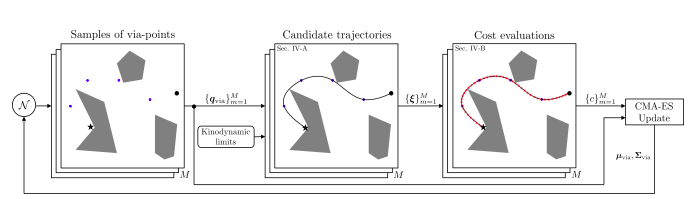
\includegraphics[scale=0.5]{figures/bl-manipulator/vpsto.png}
    \caption[The VPSTO pipeline]{The end-to-end pipeline for Via-Point Stochastic Trajectory Optimization(VP-STO). Source: \cite{VPSTO}}.
    \label{fig:vpsto}
\end{figure}


Here $s_n$ denotes the scaled via point timings $s_n = t_n/T$, which are uniformly distributed between $(0,1)$. $q(s)$ is a weighted sum of basis functions. $T$ is the total movement duration. Now, given the via-points $q_{via}$ and the boundary conditions $q_0$, $v_0$, $q_T$, $v_T$, the computation of the explicit continuous trajectory only depends on $T$. VPSTO approximates $T$ by solving for the minimum positive duration such that the resulting velocity and acceleration limits are satisfied over a discrete set of evaluation points uniformly distributed in the continuous time-space. 

For each evaluation point $s_k$, there exists a closed-form solution $T_k$ such that the motion happens through $q_0$, $q_T$, $q_{via}$, and the robot arm reach either the velocity limit or the acceleration limit at time $t = s_k$. VPSTO then picks the most conservative duration among the $K$ solutions for $T: T(q_{via}) = max(T_k)$ in order to make sure that the velocity and acceleration constraints are satisfied at all evaluation points. Once $T$ is known, $q(s)$ is found using the equations for $q_0$, $q_T$, $q_{via}$, $v_0$, and $v_T$. 

VPSTO optimizes the trajectory by minimizing a cost function that captures the tradeoff between smoothness, efficiency, and safety. Based on the design of the cost function that VPSTO minimizes, we can adapt it for a wide variety of applications. In this dissertation, we adapt the VPSTO algorithm for manipulator pushing tasks on a tabletop and pair it with a low-level push controller in Section \ref{sec:bi-level-method}.

\subsection{Collision Detection}

Collision detection for a robot manipulator needs to be performed on two fronts - self-collision, which involves collisions among the links of the robot itself, and environment collision, which includes collisions between the robot links and objects in the environment. Note that the contact between the robot's end-effector and the target object to be moved on the table is not considered as a collision. We have already discussed standard distance-based collision avoidance for manipulators in Section \ref{sec:distance-based-collision}. Let us now analyze the drawbacks of these existing approaches. 

As discussed in Section \ref{sec:distance-based-collision}, one way of checking for collisions is to sample points uniformly along the robot body and compute pairwise distances among them(for self-collision) and with other objects in the environment. If the computed distance exceeds the threshold separation determined by the geometries of the robot body and the objects, the point is collision-free. The difficulty with this approach arises due to its reliance on the knowledge of the exact geometries of the robot and the other objects. This makes it hard to generalize this approach across a range of objects of different shapes and sizes on the table, as well as to robots with different dynamics. Learning implicit representations of objects also runs into the same generalizability issue, and thus the necessity of a standardized approach capable of detecting collisions agnostic to object and robot geometries becomes evident. 

\subsubsection{PyBullet Mesh Overlap:}
In this chapter, we will adopt a different approach called 
\textit{Mesh Overlap}, that attempts to solve this problem of collision avoidance in a simulator setting. The simulator of our concern is PyBullet, which is a physics simulation engine that can be used to simulate robots and other complex systems in 3D. To use PyBullet to load 3D robots into a simulation scene, one can follow this  general sequence of steps:

\begin{enumerate}
    \item \textit{Define the robot model:} Start by defining the geometry, mass, and other properties of each link and joint in the robot model. This can be done using the URDF (Unified Robot Description Format) file format.
    \item \textit{Load the robot model:} Once we have defined the robot model, we can load it into PyBullet using the loadURDF function. This function takes as input the path to the URDF file and returns a unique identifier for the robot in the simulation.
    \item \textit{Visualize the robot:}\label{point:vis_robot} we can visualize the robot in PyBullet using the render function. This function generates a 3D mesh of the robot model and displays it in a window.
    \item \textit{Simulate the robot:} We can simulate the robot's behavior by applying forces and torques to its joints using the \verb_`setJointMotorControl2'_ function. This function allows we to specify the desired position, velocity, or torque for each joint in the robot model.
    \item \textit{Collect data:} During the simulation, we can collect data on the robot's position, velocity, and other properties using the \verb_`getBasePositionAndOrientation'_ and \verb_`getJointState'_ functions. This data can be used for analysis and control purposes.
\end{enumerate}

As discussed in point \ref{point:vis_robot}, the simulator contains the robot model as a set of geometric meshes. Similarly, for objects in the environment, the simulator loads geometric meshes into the scene. An overlap between two object meshes indicates a collision between them. We can, thus, detect collisions using PyBullet's inbuilt collision detection feature based on the overlap between the meshes of the robot and the obstacles or between the meshes of robot links. In fact, PyBullet is equipped with the feature to detect collision by detecting mesh overlap and penetration depth between meshes through the function \verb_{getCollisionFn}_. An example of mesh overlap and subsequent collision detection in PyBullet is depicted in Figure \ref{fig:collisions-pybullet}.

\begin{figure}[ht]
    \centering
    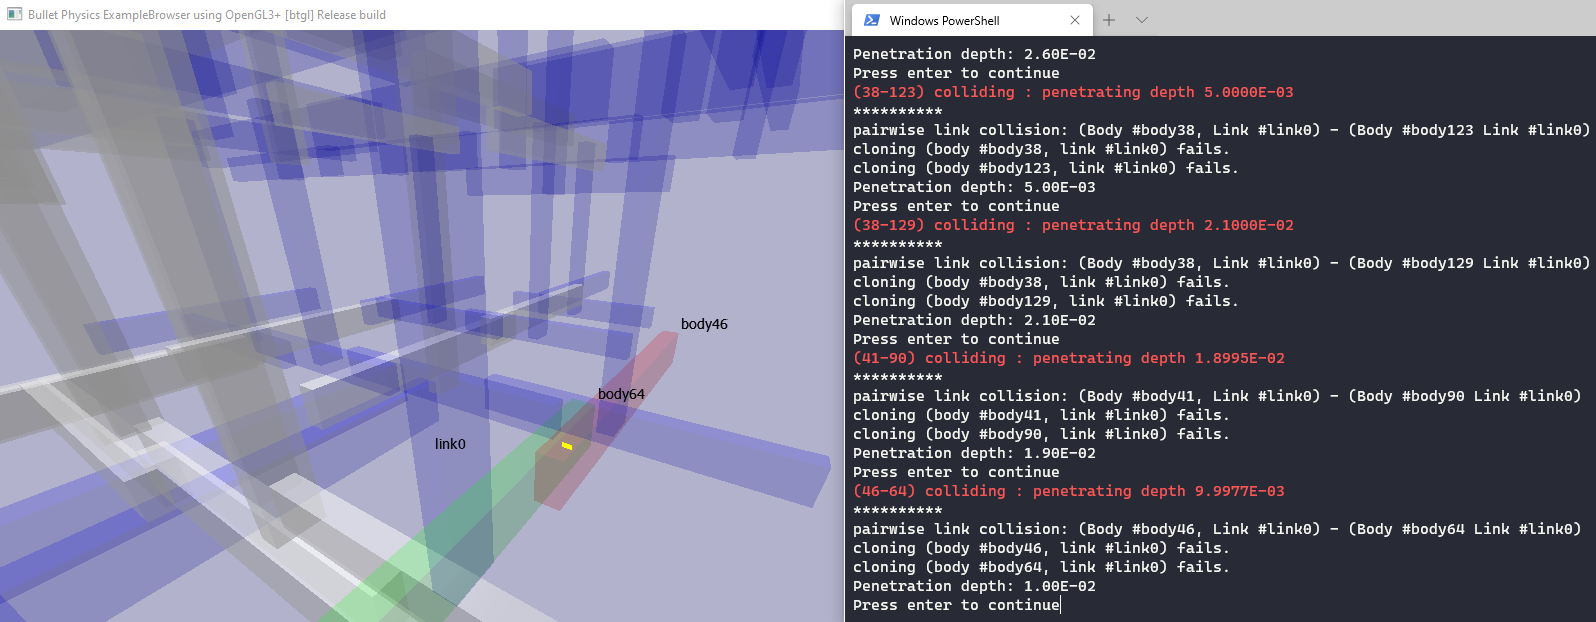
\includegraphics[scale=0.3]{figures/bl-manipulator/assembly_collision.png}
    \caption[Collision detection through Mesh Overlap]{Collision Detection through Mesh Overlaps in the PyBullet simulator. Source:  \scriptsize{\url{https://github.com/yijiangh/pybullet_planning_tutorials}}}
    \label{fig:collisions-pybullet}
\end{figure}

To explain PyBullet's inbuilt collision detection through code, let us analyze the standard use of the \verb_getCollisionFn_ as follows:

\begin{verbatim}
    collision_fn = get_collision_fn(robot, ik_joints, obstacles, 
    self_collisions=True, disabled_collisions=self_collision_links)
    print (collision_fn(joint_poses, diagnosis = True))
\end{verbatim}

We send the robot model, list of movable joints, and list of obstacle models to the \verb_getCollisionFn_, along with a few Boolean flags. \verb_selfCollisions_ indicates whether to detect self-collisions among the robot link meshes, \verb_disabledCollisionFn_ relaxes the collision detection between mesh pairs that are not counted as a collision, for example, between the end-effector and the target object being moved. \verb_getCollisionFn_ returns a Boolean flag for a given snapshot of joint poses, indicating whether it has been able to detect a collision or not. The \verb_diagnosis_ flag indicates whether we want to visualize the detected collision in the PyBullet GUI or not.

\subsection{Joint-Space Path Planning}\label{sec:joint-cost}

The design of the cost function for VPSTO determines its application to the task at hand. For non-planar end-effector motion, such as grasping and pick-and-place operations, we perform global path-planning in the joint angle space. Recall from Section \ref{sec:bg-manipulator-kinematics} that the Franka Emika Panda robot has 7 movable joints, while the UR5e robot has 6 movable joints. To represent the joint angle movements and perform path-planning in the joint space, therefore, we would need to plan in 7-D for the Franka Panda manipulator and in 6-D for the UR5e manipulator. Joint-space planning allows us to also introduce joint limits as constraints into the optimization problem based on the robot dynamics. Note that we are allowed to design discontinuous non-differentiable cost functions since VPSTO never computes the gradient of the cost function but relies on stochastic optimization. We design a cost function for VPSTO as a sum of the following terms:

\begin{enumerate}
    \item \textbf{Cost Limits}: This is defined as the frequency of violation of joint limits while executing a joint-space trajectory. 
    \item \textbf{Cost curvature}: Curvature cost aims to shorten the arc length (refer to Section \ref{sec:traj_eval_metrics} for arc-length definition) of the joint-space trajectory to ensure short trajectories. 
    \item \textbf{Joint Cost}: Joint cost is defined as the norm of the difference in joint angles over successive timestamps. In essence, joint cost captures the effort expended by the robot to perform some task by changing its joint angles. 
    \item \textbf{Cost Collision}: This is a discrete cost, consisting of a very high-cost value $C$ if a collision is detected, or 0 otherwise. 
    \begin{equation}
        \text{Collision Cost} = \begin{cases} 
      C & \text{if collision = True} \\
      0 & \text{otherwise} 
   \end{cases}
    \end{equation}
    
\end{enumerate}

\subsection{Simulation Results for Joint-Space Path Planning}

We test the VPSTO-based global joint-space path planner using the cost function defined in Section \ref{sec:joint-cost} in PyBullet for a few scenarios involving one or two obstacles of varied sizes. The results of a few test simulations can be found at: \url{https://www.dropbox.com/scl/fo/t1dy47cgz2rvmedj9a87o/h?dl=0&rlkey=ou4losxv0i9lawc2wffnk60vl}. Figure \ref{fig:joint_traj_ur5} shows an example trajectory from our simulator runs for the Universal Robots UR5e robot arm. 

\begin{figure}[ht]
    \centering
    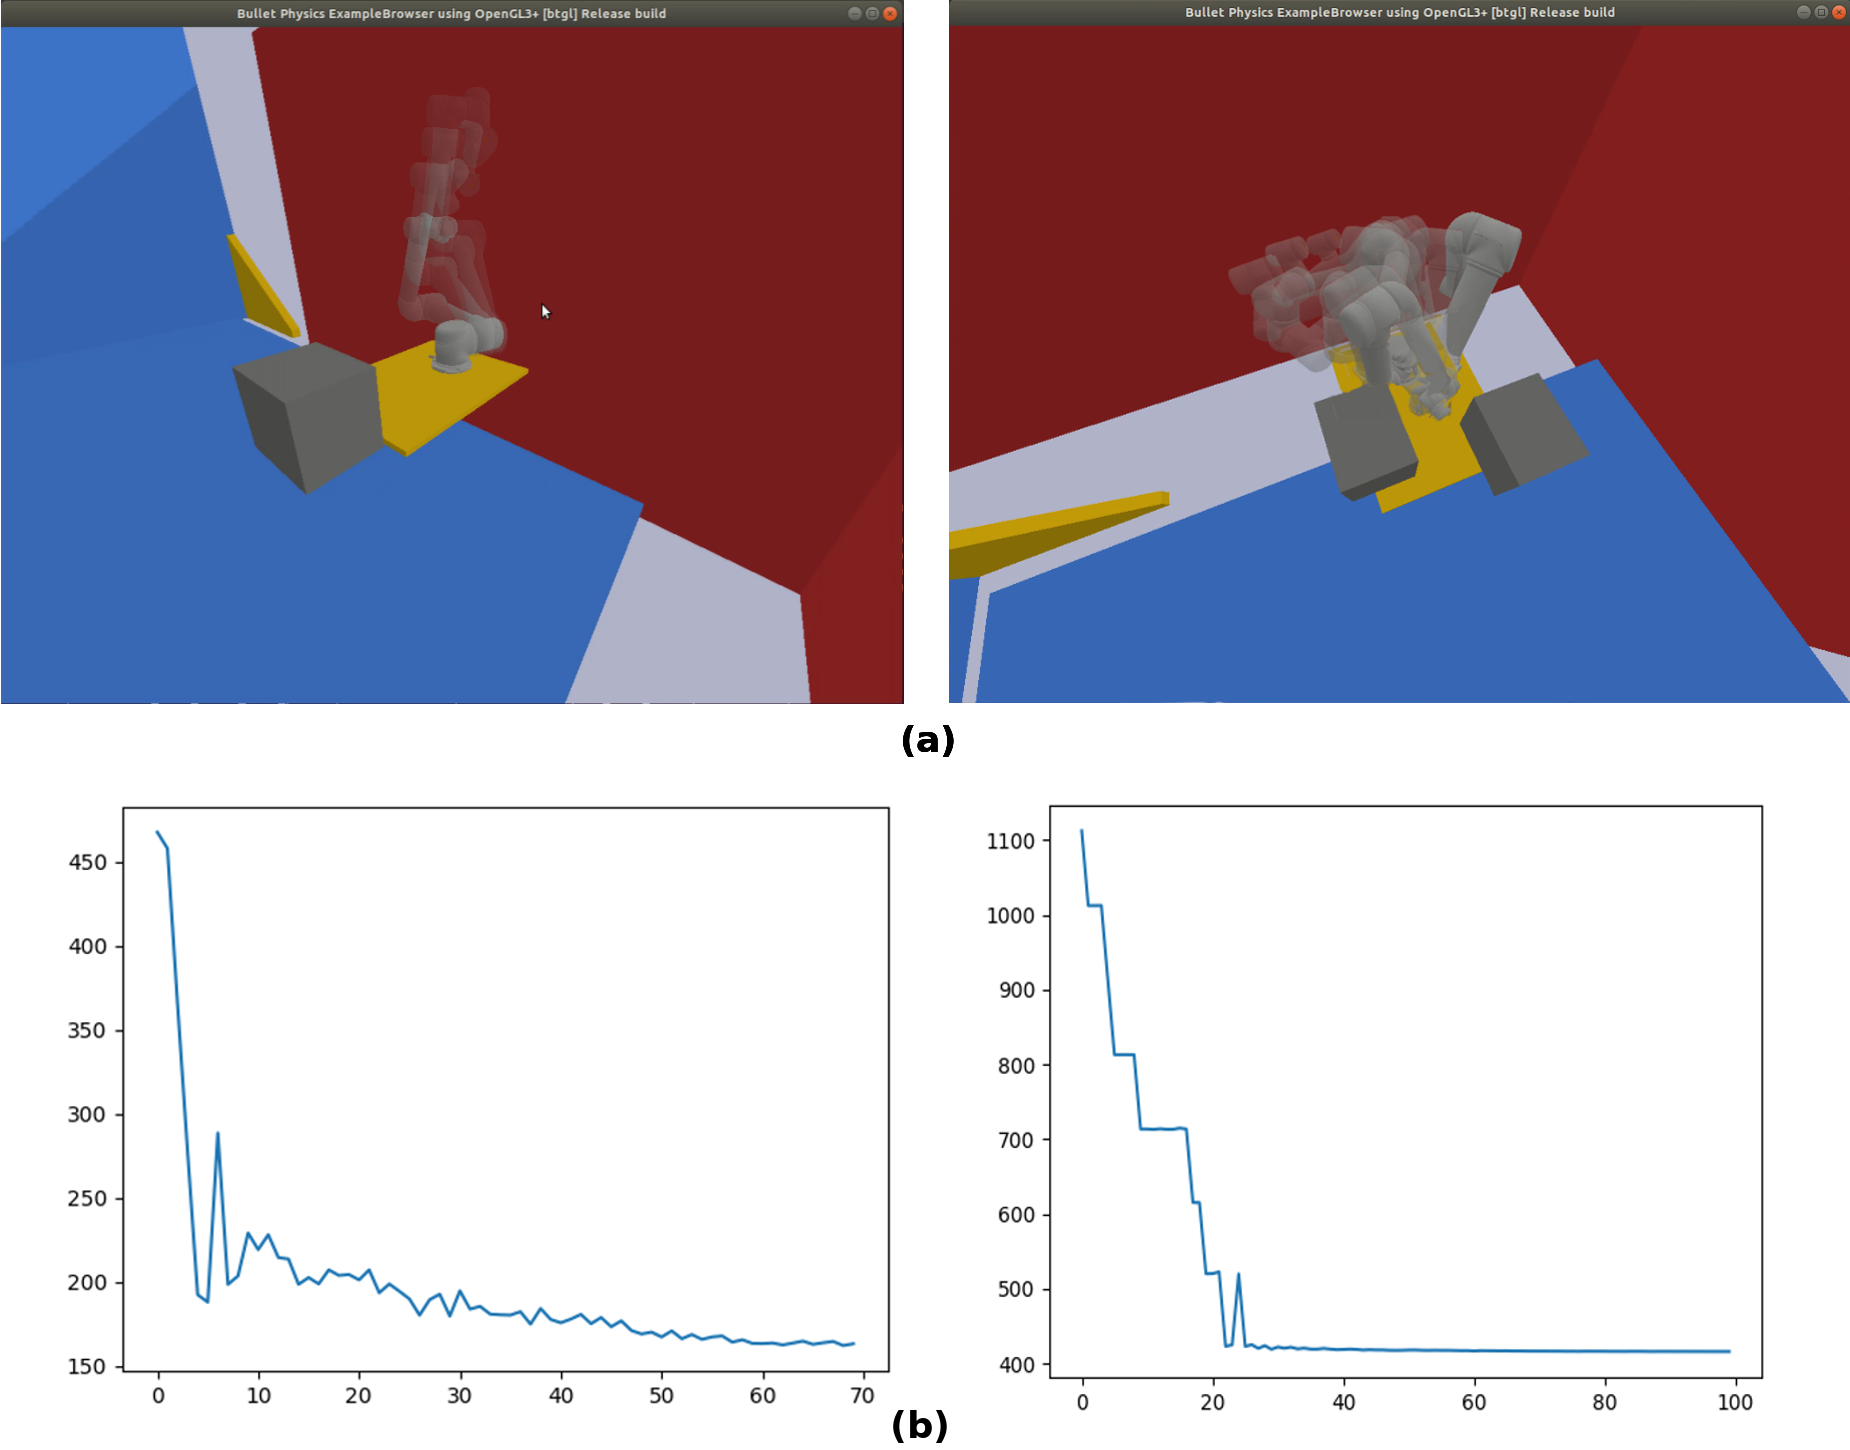
\includegraphics[scale=0.2]{figures/bl-manipulator/joint_trajs.png}
    \caption[Joint-space trajectories using VPSTO]{(a) A few examples of trajectories obtained after joint-space trajectory optimization using VPSTO simulated in PyBullet. (b) The associated cost function plots during the optimization iterations. VPSTO is able to minimize the cost function, which can be denoted by the reducing trend in the cost plots.}
    \label{fig:joint_traj_ur5}
\end{figure}

\subsection{Path Planning for Pushing Objects on a Table}

For the planar motion of the manipulator's end-effector, such as pushing an object along a table, we can discard the high-dimensional joint space path planning in favor of a simpler Cartesian-space motion of the end-effector. Thus the path planning for the end-effector can be performed in the Cartesian end-effector space, which would be 2-D in the case of planar tabletop motion. The end-effector can be thought of as a circular holonomic robot in 2-D of diameter equivalent to the separation between the fingers of the gripper plus the finger widths. This approximation makes it possible to use standard holonomic robot path-planning algorithms, as well as stochastic optimizers like VPSTO, to plan the end-effector trajectory. We can further simplify this by planning 2-D trajectories for the center of the object being pushed on the table instead of directly the end-effector, particularly in cases where only brief contacts or pushes by striking are allowed between the end-effector and the object. In such cases, it is not enough for the end-effector to reach the desired goal position. Rather, the object should be able to reach the goal position, and an efficient push controller should be designed to determine the controls necessary for the manipulator to push the object along the planned trajectory. An example of a 2-D trajectory for an object being pushed on a table by a manipulator is shown in Figure \ref{fig:end-eff-traj}.

\begin{figure}[ht]
    \centering
    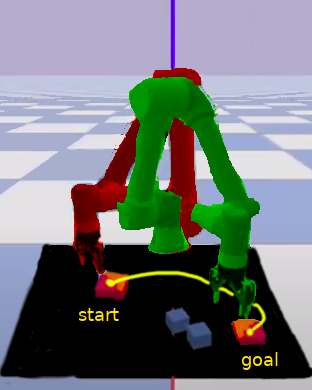
\includegraphics[scale=0.5]{figures/bl-manipulator/end_eff_traj.png}
    \caption[2-D Trajectory of an object being pushed by a Manipulator]{2-D Trajectory of an object being pushed by a Manipulator. Here the red-shaded manipulator denotes its start pose, and the green-shaded manipulator denotes its final pose. The blue cubes indicate obstacles (collision objects) on the table. The end-effector motion happens along the plane of the black table as the object moves from the start to the goal position. The yellow line denotes the trajectory of the center of the object being pushed.}
    \label{fig:end-eff-traj}
\end{figure}

\subsubsection{Analysis of Joint Costs associated with Cartesian-space trajectories for pushing objects}

For manipulators, in addition to the performance metrics discussed in Section \ref{sec:traj_eval_metrics}, joint cost becomes a very important metric for benchmark comparison. Joint cost is defined as the norm of the difference in joint angles over successive timestamps. In essence, joint cost captures the effort expended by the robot to perform some task by changing its joint angles, and therefore, the goal of an efficient trajectory optimizer would be to minimize the joint cost incurred by the robot arm to complete a given task. For joint-space path planning, it is easy to incorporate the differences between successive joint angles for each joint-space trajectory. However, if we are planning in the Euclidean end-effector space, or in the space of the center of the object being pushed on the table, minimizing just the Euclidean length of the trajectory may not be sufficient; it is important to check for the joint effort to execute an end-effector trajectory or push an object along a planned trajectory. Table \ref{table: straight-line-vs-joint} demonstrates that the shortest object-center trajectory in terms of Euclidean length, i.e. straight-line trajectory, does not always guarantee the least joint cost; in fact, the trajectory returned by VPSTO optimizing over joint-cost is more optimal in terms of joint effort for the same number of waypoints. To compute joint cost, we need to execute the planned object-center trajectory using a push controller and obtain the joint angles. For real robots, we can use manipulator-specific analytical Inverse Kinematics(IK) solvers\cite{Analytical_IK} to convert end-effector positions to joint angles. 

\begin{table}
\centering
\caption{Comparison of Joint Costs associated with different types of object-center trajectories using our push controller from Section \ref{sec:low-level-rl}.} \label{table: straight-line-vs-joint}
\scriptsize
\begin{tabular}{|p{2cm}|p{2cm}|p{4cm}|p{2cm}|p{3cm}|}\hline
 Start Position(m,m) & End Position(m,m) & Trajectory Type & Num WayPoints & Joint Cost
\\ \hline
(0.35, -0.05) & (0.5, 0.1) & Straight line & 8	& 48.0866966147044 
\\ \hline
(0.35, -0.05) & (0.5, 0.1)	& 2-piecewise straight lines & 8 & 53.2750370301563
\\ \hline
(0.35, -0.05) & (0.5, 0.1)	& VPSTO		& 8	& 	39.5423031834928
\\ \hline
(0.4, -0.15) & (0.63, 0.05)	& Straight line	& 8	& 83.0072021138549
\\ \hline
(0.4, -0.15) & (0.63, 0.05)	& 2-piecewise straight lines & 8 & 113.146020007934
\\ \hline
(0.4, -0.15) & (0.63, 0.05)	& 3-piecewise straight lines & 8 & 115.673830244566
\\ \hline
(0.4, -0.15) & (0.63, 0.05) & 4-piecewise straight lines & 8 & 120.5008919817
\\ \hline
(0.4, -0.15) & (0.63, 0.05)	& VPSTO	& 8	& 62.1512468250956
\\ \hline
(0.5, 0.1)	& (0.65, -0.05)	& Straight line	& 18 & 88.1713855670522
\\ \hline
(0.5, 0.1)	& (0.65, -0.05)	& 2-piecewise straight lines & 18 & 100.889302118451
\\ \hline
(0.5, 0.1)	& (0.65, -0.05)	& VPSTO & 18 & 77.346373
\\ \hline
\end{tabular}
\normalsize
\vspace{-0.4cm}
\end{table}

\section{Bi-Level Optimization for Non-Prehensile Actions}\label{sec:bi-level-method}

\subsection{Introduction}
 Non-prehensile manipulation has typically received less attention in the literature compared to grasp manipulation. A standard mechanism to robustly push an object from start to goal position while avoiding colliding with objects on the table does not exist. 

A recent work~\cite{iros2022} tackles this problem but assumes contact-rich manipulation in which the target object is attached to the manipulator. This reduces the complexity of the problem by assuming predictable dynamics - the object moves along with the manipulator. Contact-rich manipulator, however, assumes a certain type of gripper that may not be feasible for a given use case.  We concentrate on non-prehensile manipulation in an end-effector agnostic manner that assumes the object dynamics to be independent of the end-effector dynamics. The primary challenge in developing a policy to execute such an action is the stochastic outcome of pushing an object: in the absence of privileged information like friction, the weight of the target object, it is impossible to accurately predict the dynamics of the object on a push action. To tackle this, several works have tried to explicitly model the outcome by training a deep neural network on a large amount of push-outcome pairs collected via simulation~\cite{huang2021dipn, huang2021visual, bai2021hierarchical-more}. However, such explicit modeling results in low generalization, making multi-step long-horizon planning of pushing an object from start to goal challenging. 

In recent years, deep reinforcement learning (RL) has shown promising results in various robotics applications. RL algorithms learn to perform a task by maximizing a reward signal, which can be a scalar value that reflects the task's success or failure; or a dense reward indicating the distance from the goal. However, RL algorithms have high sample complexity~\cite{rl_sample_complexitiy}, and designing the perfect reward function is tricky, limiting their application in long-horizon scenarios~\cite{rl_long_horizon} needing complex reward design. 

Moreover, RL algorithms trained for long-horizon tasks are hard to generalize across a wide variety of scene configurations and out-of-distribution object shapes and sizes.

In this work, we tackle the problem of object rearrangement using non-prehensile actions by disentangling the space of control and planning. The path planning module generates a feasible trajectory for the robot's end-effector, while the low-level RL controller learns to control the robot's movements to achieve the desired task. In our framework, RL acts as an efficient mechanism for understanding the dynamics of an object on different push actions. Here, the RL controller is trained using a simple objective to push the object quickly to a given goal location. 

In this setting, the low-level controller is unaware of the collision objects and is dependent on a high-level planning module to obtain an optimal collision-free trajectory. At the same time, the high-level planning module predicts the most optimal trajectory for the given RL controller. The framework is trained using bi-level optimization: the high-level planning module is optimized on the cost of execution of the low-level controller. 

A global RL policy solves the task of manipulating an object from start to goal position end-to-end using a single policy. Such a controller simultaneously solves the control task (understanding the dynamics of the system) and the planning task (a collision-free optimal trajectory from start to goal). 
Compared to training a global RL model for non-prehensile object manipulation, our framework, based on a bi-level optimization objective can have several advantages: 

\begin{enumerate}
    \item \textbf{Better task-specific performance:} Non-prehensile object manipulation tasks can be highly varied and complex, and a single global RL model may not be able to handle all tasks equally well. In contrast, a bi-level optimization approach can generate task-specific plans that are optimized for each individual task, resulting in better performance. 
    \item \textbf{Improved sample efficiency:} Non-prehensile object manipulation tasks typically require a large number of samples to train an RL model effectively. A bi-level optimization approach can reduce the number of samples required by using the high-level planning module to generate a task-specific collision-free plan, which can simplify the RL objective to only push to a goal location. 
    \item \textbf{Better interpretability:} A bi-level optimization approach separates the control of the task-specific plan and the low-level actions, making it easier to understand how the system operates and diagnose issues. In contrast, a global RL model can be more opaque and difficult to interpret. 
    \item \textbf{Ability to handle constraints:} Non-prehensile object manipulation tasks often have constraints, such as avoiding collisions or maintaining balance. A bi-level optimization approach can incorporate these constraints into the high-level planning module and use them to guide the low-level actions. 
\end{enumerate}

In contrast, a global RL model may struggle to handle constraints effectively, as designing an appropriate reward can be tricky. 

\subsection{Related Work}

Push-based non-prehensile manipulation can be divided into push-to-grasp, such as pushing objects in clutter to make them graspable~\cite{huang2021dipn, huang2021visual} or sliding an object to the edge of the table~\cite{pregraspsliding, King-2013-7735} and push-to-goal to push an object from a start to a goal position~\cite{iros2022, icra2018, moura2022non, bai2021hierarchical-more}. The latter line of work can further be classified as contact-rich manipulation either by sliding by the top~\cite{xu2021cocoi, song2019object, icra2018, iros2022} or by the side~\cite{moura2022non}. 

We aim to tackle push-to-goal through push-by-striking manipulation. Push-by-striking loses the contact-rich assumption and thus disentangles the dynamics of the object from the manipulator dynamics removing the constraints in the type of end-effector - as the end-effector strikes an object, the outcome of the object state is independent of the end-effector state. 

RL has been applied in various robotics applications, including grasping~\cite{grasp1, grasp2,grasp3}, manipulation~\cite{manipulation1, manipulation2}, and locomotion~\cite{locomotion1, locomotion2}. Recently there has been a lot of work~\cite{residual1, residual2, residual3} on combining RL with classic controllers and primitives to improve their performance. RL-based methods have also shown promising results in performing non-prehensile object manipulation tasks. For instance, Tan et al.\cite{hierarchical-rl} proposed a hierarchical RL method for non-prehensile object manipulation, where the high-level policy generates a sequence of subtasks, and the low-level policy learns to execute each subtask. Zhang et al.\cite{zhang-rl} proposed a hierarchical RL framework that combines the advantages of both model-based and model-free methods for non-prehensile object manipulation.

Path planning algorithms are also widely used in robotics applications, including object manipulation~=\cite{planning1, planning2, planning3}. Path planning algorithms generate a feasible trajectory for the robot to perform the task. Various path-planning algorithms have been proposed, including sampling-based methods\cite{planning1} and optimization-based methods\cite{planning2}. While other path-planning approaches would build a path without taking into account the capabilities of the lower-level controller, our trajectory optimization model samples optimal trajectories by considering the capability of our low-level RL controller. Our neural network is aware of the limitations and capabilities of the lower-level RL controller. 

\subsection{Task Specification}
\label{sec:task-specification}

We consider the task of pushing a target object from an initial pose to a goal pose on a tabletop scene with multiple movable collision objects. The environment consists of a planar surface with dimensions of 0.8m $\times$ 0.8m, upon which up to four movable objects are randomly placed. The target object is a rectangular block with dimensions 0.05m $\times$ 0.05m $\times$ 0.1m, and the robot manipulator is a Franka-Panda arm with a two-fingered gripper; however, our framework is independent of the type of gripper and can be extended to any end-effector setting (point contact, area contact, contact-rich, etc.). The manipulator interacts with the environment by pushing the target object, using the tip of the arm as the pushing point. The goal location is specified as the pose of the target object on the given tabletop scene. 

\subsection{Proposed Framework}

Our proposed approach involves two modules: a path-planning module and a low-level RL controller. The path planning module generates an optimal collision-free trajectory for the robot's end-effector, while the low-level RL controller controls the robot's movements to accomplish the task objectives. Fig.~\ref{fig:pipeline} illustrates the proposed approach.

\begin{figure}
    \centering 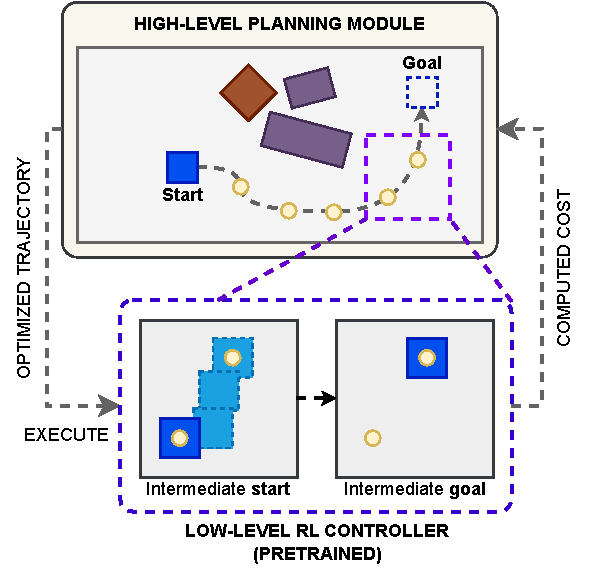
\includegraphics[scale=0.8]{figures/bl-manipulator/pipeline.v9.pdf} 
    \caption[Bi-level optimization pipeline]{Our bi-level optimization framework solves the task of non-prehensile object manipulation in a cluttered tabletop rearrangement scene. We make use of a low-level RL controller that is trained to reach a short goal. The high-level planning module predicts a set of waypoints that is most optimal for the low-level RL controller to execute. The purple and brown objects indicate obstacles (collision objects); dark-blue squares indicate the target object, and the light-blue squares indicate the trajectory taken by the RL controller between a set of intermediate waypoints predicted by the high-level planning module.}
    \label{fig:pipeline}
\end{figure}

\subsubsection{Low-level RL Push Controller}
\label{sec:low-level-rl}

Our RL controller learns to simply push a target object from a start to a goal location on a tabletop scene. Our controller is trained without any obstacles on the table and is optimized to approach the goal location quickly. Our state space consists of the set of poses taken by the target object, which is being pushed by the RL controller. The action space is defined as a set of 8 discrete equidistant points on the perimeter of the target object and 8 different push angles at each of these 8 points. The objective of the controller is to learn a policy that maximizes the expected cumulative reward, where the reward is the dense negative distance from the current pose to the goal location. The distance metric is the Euclidean distance between the centroid of the target object and the goal location.

Formally, the state space is represented by $S \in \mathbb{R}^{6}$, where each element of the state vector represents the position and orientation of the target object. The action space is represented by $A \in \mathbb{R}^{16}$, where each action is a combination of a point on the object and a push angle. Let $s_t \in S$, and $a_t \in A$ denote the state and action at time step $t$, respectively. The state transition is deterministic, and the next state $s_{t+1}$ is computed as the result of applying the push action to the current state $s_t$.

The reward function is defined as 
\begin{equation}
r(s_t, a_t) = -\gamma ||\; \mathcal{C}(s_t) - \mathcal{G}\; ||_2
\end{equation}
where $\gamma$ is a discount factor, $\mathcal{C}(s_t)$ is the centroid of the target object in the current state, and $\mathcal{G}$ is the goal location. The negative distance metric is used to encourage the controller to minimize the distance to the goal location. The discount factor is used to balance the trade-off between short-term and long-term rewards.

The RL controller learns a policy $\pi(s_t)$ that maps states to actions by maximizing the expected cumulative reward. The optimal policy is obtained by solving the Bellman equation, which is given by:
\begin{equation}
\begin{aligned}
    &Q(s_t, a_t) = r(s_t, a_t) \\
    &+\; \gamma \sum_{s_{t+1}} P(s_{t+1}|s_t,a_t) \max_{a_{t+1}} Q(s_{t+1}, a_{t+1})
\end{aligned}
\end{equation}
where $Q(s_t, a_t)$ is the state-action value function, $P(s_{t+1}|s_t,a_t)$ is the transition probability, and $\max_{a_{t+1}} Q(s_{t+1}, a_{t+1})$ is the maximum expected future reward. The policy is then derived from the optimal value function as:
\begin{equation}
    \pi(s_t) = \arg\max_{a_t} Q(s_t, a_t)
\end{equation}

To learn the optimal policy, we employ a deep Q-learning algorithm that uses a neural network to approximate the value function. The network takes the state as input and outputs the value for each action in the action space. We use the Adam optimizer to minimize the mean squared error between the predicted and target Q-values.

\subsubsection{High-Level Path Planning Module}
\label{sec:path-planning-module}
The high-level planner generates a feasible trajectory for the object being pushed by the manipulator, taking as input the initial and final configurations of the object and producing a sequence of intermediate via points that the low-level controller must push it along. In our case, it is important to plan the high-level trajectory for the object instead of the manipulator itself, as is done in the case of contact-rich manipulation. This is because the behavior of the manipulator and the object being pushed are different. Pushing in a contact-impoverished manipulation task, the robot's end-effector only contacts the object briefly to give it a push, and the object continues to move without being directly contacted by the manipulator. Due to this, it is not straightforward to predict the object's trajectory based solely on the manipulator's motion, making it more challenging to plan a trajectory directly for the manipulator. It is noteworthy that planning the high-level trajectory for the object, as opposed to the manipulator, provides a robust and gripper-agnostic algorithm that accounts for the mismatches between the manipulator's motion and the object's movement due to striking.

The predicted via points are collision-free and ensure that the object can be pushed toward the goal location without encountering any obstacles. For high-level planning, we use the VPSTO algorithm, a stochastic sampling-based optimization method. VPSTO evaluates candidate trajectories by estimating the per-iteration cost function on a simulator running the low-level RL controller, which effectively captures the manipulator and environment dynamics. The cost function incorporates joint cost, collision cost, and boundary cost, as explained in the following section.

\subsection{Designing the bi-level optimization objective}

As can be seen in Fig.~\ref{fig:pipeline}, the high-level planning module predicts an optimal trajectory for the end-effector. In other words, the predicted trajectory, $\mathcal{T}$, comprising of a set of via-points, $\mathcal{V}$, is optimal in terms of the manipulator's joint cost, $\mathcal{J}$, as it tries to execute the trajectory. 

To obtain the optimal trajectory for a given scene made of multiple obstacles, VPSTO optimizes the following cost objective, $\mathbb{J}$ computed as:
\begin{equation}
    \mathbb{J}(\pi, \mathcal{V}) = \alpha\mathcal{J} + \beta\mathcal{X} + \gamma\mathcal{B} 
\end{equation}
where $\pi$ is our low-level RL policy as defined in Sec.~\ref{sec:low-level-rl}. $\mathcal{X}$ and $\mathcal{B}$ are the collision and out-of-boundaries cost, respectively. $\alpha$, $\beta$, and $\gamma$ are the scaling parameters to normalize the three different metrics.  $\mathcal{J}$ is calculated based on the first-order change in the manipulator's joint angles, while the collision cost, $\mathcal{X}$, reflects the change in obstacle positions in the scene. The out-of-boundary cost, $\mathcal{B}$, is calculated as the frequency of workspace boundary violations. Note that the joint angles are obtained after simulating the manipulator's movement using the low-level RL controller in PyBullet. For each of the via-point $\{v_i\}_{i=1}^{\mathcal{K}-1} \in \mathcal{V}$, the RL controller is executed to push the object from $v_i$ to $v_{i+1}$; here $\mathcal{K}$ is the number of via-points predicted by the planning module. The total joint cost is then computed as:
\begin{equation}
\label{eqn:joint-cost}
    \mathcal{J} = \sum_{i=1}^{\mathcal{K}-1} j(v_i, v_{i+1})
\end{equation}
where $j$ indicates the local cost of moving the target object between the intermediate via points. Furthermore, our approach mainly focuses on the pushing behavior of the manipulator on the plane of the table; collisions can be assumed to be marked by positional displacements of obstacles according to the task specification in Section~\ref{sec:task-specification}.

\subsection{Simulation Results}\label{sec:bl_results}

We test our bi-level optimizer on a few tabletop scenarios involving one or more obstacles of varied shapes and sizes in the PyBullet simulator. Figure \ref{fig: bl_qualitative} shows the trajectories predicted by our bi-level approach while avoiding collisions and minimizing joint cost within the workspace bounds. Figure \ref{fig:bl_sim} indicates the predicted trajectory when run in the PyBullet simulator using our low-level push controller. Additional simulation results on other test cases can be found at \url{https://www.dropbox.com/sh/mf8j0kq4mv53wct/AABVdITIHCfNBtqHMphnJcSia?dl=0}.


\begin{figure*}
    \centering 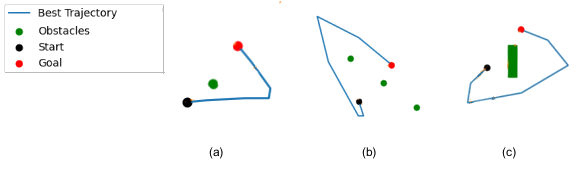
\includegraphics[width=0.8\linewidth]{figures/bl-manipulator/trajectories-v2.png} 
    \caption[Bi-level optimizer trajectories]{Trajectories predicted by our framework. Our framework successfully avoids trajectories and is conservative when choosing a path. Note that the positions shown here are placeholders to indicate the locations of the centers of various objects. (a) shows a trajectory with a simple case of a single collision object, and (b) shows a more complicated case when there are multiple collision objects. The obstacle sizes are so big that it is not possible for the manipulator to go between them, so it takes an alternate route around the obstacles. (c) shows a case with an elongated obstacle. Even though the trajectories may not look the most optimal in terms of Euclidean distance, these trajectories are near-optimal with respect to joint and collision costs. Refer to Table \ref{table: straight-line-vs-joint} for the analysis of joint costs vs Euclidean distance for 2-D trajectories.}
    \label{fig: bl_qualitative}
\end{figure*}

\begin{figure*}[t!]
    \centering
    \begin{subfigure}[t]{0.5\textwidth}
        \centering
        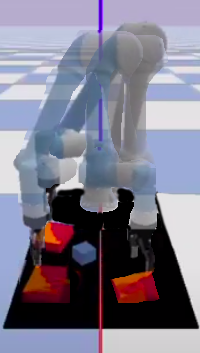
\includegraphics[height=1.8in]{figures/bl-manipulator/bl_sim.png}
    \end{subfigure}%
    ~ 
    \begin{subfigure}[t]{0.5\textwidth}
        \centering
        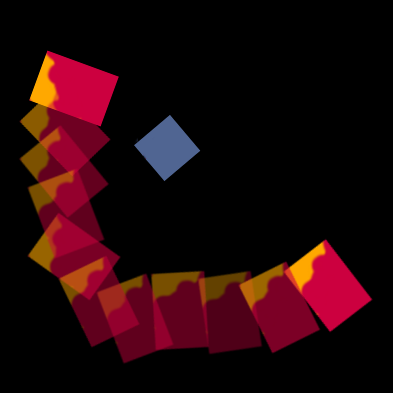
\includegraphics[height=1.8in]{figures/bl-manipulator/2d_object.png}
    \end{subfigure}
    \caption[Bi-level simulation in PyBullet]{(a) Trajectories predicted by our framework simulated in PyBullet with our low-level RL push controller. The blue boxes on the black table indicate collision objects(obstacles), and (b) The top-view of the object motion as a result of executing the trajectory.}
    \label{fig:bl_sim}
\end{figure*}

\section{Discussions and Conclusion}

In this chapter, we adapted the Via-point-based Stochastic Trajectory Optimization(VPSTO) trajectory optimizer for manipulator path planning tasks, using PyBullet's mesh overlap technique to detect collisions. We presented a few simulation results obtained from joint-space trajectory planning using VPSTO. We then proposed a framework for disentangling non-prehensile long-horizon manipulation into planning and control. Our approach predicts a collision-free trajectory using VPSTO and simplifies the control component's task by reducing it to moving the object toward the next via point. In the future, one can reduce the planning time for our offline bi-level optimizer by curating a dataset of start-goal pairs and their optimal trajectories. A neural network can be trained to learn these configuration-to-trajectory mappings and can be used in real-time during inference to quickly obtain optimal manipulator trajectories. Further, more ablation studies can be performed by replacing the optimizer and the push controller in our bi-level optimization framework. Overall, our proposed framework is a promising step towards achieving more efficient and flexible non-prehensile manipulation.

%--------------------------------------------------------

\chapter{Conclusions}
\label{ch:conc}
This dissertation discusses various optimization techniques for the high-dimensional trajectory optimization of robots. We tackle two complex robot systems - multi-robot systems with a large number of robots planning start-to-goal collision-free trajectories and robot manipulators operating in $n$-dimensional joint spaces formed by $n$ joints. By suitable design of objective functions, choice of optimization paradigm, and mathematical approximations, our proposed path-planning methods aim to solve otherwise computationally intractable trajectory optimization problems. We present two major contributions - a GPU-accelerated distributed multi-agent trajectory optimizer and a stochastic trajectory optimizer for robot manipulators. 

For the GPU-accelerated multi-agent trajectory optimizer, we leverage parallelism offered by GPUs and mathematical reformulations to convert a complex Quadratic Programming(QP) optimization problem into a simple set of matrix-matrix products. We have outperformed existing state-of-the-art algorithms in various multi-robot planning scenarios with varied numbers of robots, obstacles, and their configurations. Beyond just computational acceleration, we also achieve comparable trajectory quality against our benchmarks and show how our optimizer achieves an improving performance gap with respect to them as the complexity of the planning task increases. 
\footnote{The software package for our GPU-accelerated distributed multi-robot optimizer has been made publicly available at \url{https://github.com/susiejojo/distributed_GPU_multiagent_trajopt}.}

For manipulator trajectory generation, we adapt the existing Via-Point based Stochastic Trajectory Optimization(VP-STO) method with a suitably-designed cost function to plan collision-free paths in the joint space. We leverage PyBullet's mesh overlap-based collision detection to design our collision cost function. We demonstrate the efficiency of our approach through simulations in PyBullet for different manipulators such as UR5e and Franka Emika Panda. We then couple this high-level path planner with a low-level Deep Reinforcement Learning(RL) based push planner to solve the non-prehensile task of pushing an object on a 2-D tabletop. We present results obtained from the bi-level trajectory optimizer for different shapes and numbers of obstacles on the table. 

Beyond computational speed-up, we demonstrate in Section \ref{sec:appendix-RVO} and \ref{sec:appendix-MAPF} a few additional applications of our multi-agent optimizer, in improving the quality of trajectories given by multi-agent collision-avoidance methods such as Reciprocal Velocity Obstacle(RVO) and Multi-agent Pathfinding(MAPF) Methods. This shows that our algorithm, when coupled with other planning algorithms as initializations, can improve the quality of trajectories planned by them. Beyond holonomic robots, our algorithm can also be extended to non-holonomic robot systems and even to high-dimensional robots such as manipulators. Similarly, our bi-level trajectory optimization algorithm for manipulators can be used as a teacher to train artificial neural networks to learn optimal paths from a given start position to an intended goal position. This approach could ultimately make the goal of real-time path planning for robot manipulators a reality. 

In the entirety, we believe that the contributions of this dissertation will help solve path-planning problems for a wide variety of complex robot systems and will serve as inspiration to enable robots to solve tasks ranging from simplifying our daily household work to industrial labor and defense applications. 


%--------------------------------------------------------

%%% Optional appendix
\appendix

\chapter{Distributed GPU-accelerated Multi-Agent Joint Trajectory Optimizer: JAX NumPy and Initializations}
\label{ch:appendix-gpu-mat}
\section{\label{appendix:JAX}JAX NumPy: Usage Tutorial}

JAX is a Python library developed by Google that provides an easy and efficient way to perform numerical computations, particularly those involving large matrices and tensors, on a GPU. JAX uses a technique called \textit{Just-In-Time (JIT) compilation}, which compiles the Python code into optimized machine code that can run on the GPU. This allows JAX to take advantage of the parallelism offered by the GPU, making computations much faster than if they were performed on the CPU.

One of the key features of JAX is its ability to automatically differentiate functions. JAX also provides a set of linear algebra operations that are optimized for GPU acceleration, including matrix multiplication, matrix-vector multiplication, and matrix inversion. To perform matrix operations using JAX, one first needs to create arrays or tensors that contain the matrix data and then use the JAX linear algebra functions to perform matrix operations on these arrays. 

The usage of the JAX NumPy library involves a minor change in standard NumPy Python code by replacing most NumPy function calls with JAX NumPy calls. For example, to define a 2-D tensor of zeroes of shape $(5,3)$ in JAX NumPy, we would do the following:

\begin{verbatim}
    import jax.numpy as jnp
    new_arr = jnp.zeros((5,3))
\end{verbatim}

To use the JIT feature of JAX NumPy, we can think of JIT as a decorator that accepts functions operating on JAX arrays and their arguments as static arguments. For example, if we have a function 'addJAX' defined over JAX NumPy arrays, we would tell the Python interpreter to use JIT compilation for this function as follows:

\begin{verbatim}
    from jax import jit
    add_jit = jit(addJAX)
\end{verbatim}

JAX NumPy does not allow tensor slicing or direct indexing but rather makes use of the C++ style `at' function to access tensor elements by index. In addition, JAX tensors are immutable, i.e. they cannot be edited in place. Please refer to the official documentation of JAX NumPy for further details on JAX methods at \url{https://jax.readthedocs.io/en/latest/jax.numpy.html}


\section{\label{appendix:GPU-acc-comparison}Comparison of different off-the-shelf GPU-based tensor manipulation libraries}

For the centralized joint trajectory optimization problem for multiple holonomic robots, we implement the path planning algorithm using three different off-the-shelf open-source Python libraries - vanilla NumPy, JAX NumPy, and CuPy. The latter two libraries use accelerated tensor computations to achieve computational speed-up in computing large tensor operations, such as matrix multiplications, inverses, and so on. As discussed in Appendix \ref{appendix:JAX}, JAX NumPy leverages GPU acceleration for CUDA-based tensor computations, and so does CuPy. Table \ref{table: gpu-acc-comp} compares the time taken to plan start-to-goal offline trajectories for a varying number of robots using the same core centralized trajectory optimization approach.

\begin{table}
\centering
\caption{Comparison of multi-agent path planning times using different mathematical libraries} \label{table: gpu-acc-comp}
\scriptsize
\begin{tabular}{|p{3cm}|p{3cm}|p{3cm}|}\hline
 Number of Robots & Planning time(in sec) & Library
\\ \hline
4 & 0.0050 & NumPy
\\ \hline
8 & 0.0049 & NumPy
\\ \hline
16 & 0.0046 & CuPy
\\ \hline
32 & 0.0046 & JAX NumPy
\\ \hline
32 & 0.267 & NumPy
\\ \hline
32 & 0.0049 & CuPy
\\ \hline
64 & 0.0047 & JAX NumPy
\\ \hline
\end{tabular}
\normalsize
\vspace{-0.4cm}
\end{table}

We observe from Table \ref{table: gpu-acc-comp} that compared to NumPy, JAX NumPy achieves a computational acceleration of around $60$ times over vanilla NumPy by leveraging GPU computations. Further, the planning time for 32 as well as 64 robots are similar, indicating that the JAX-based implementation of the algorithm remains nearly constant regardless of the increase in the number of robots, or, in other words, an increase in the size of the matrices used in the optimization process. For CuPy, we observe a similar trend in the planning time, where between 16 and 32 robots, the computation time remains nearly constant as well. 

\section{Initializations using Reciprocal Velocity Obstacle(RVO)\cite{RVO}}\label{sec:appendix-RVO}

RVO is a local, reactive multi-robot trajectory planner that has been shown to generate collision-free trajectories in real-time for hundreds of Robots\cite{RVO}. Even though it runs in real-time, RVO trajectories cannot be directly executed by Robots as they are jittery and jerky. We use a trick to precompute trajectories using RVO for given start and goal positions of multiple Robots and use the RVO trajectories along with other optimizer parameters computed from them to initialize our optimizer. Thus the task of eliminating collisions is first performed by RVO and further enhanced by our optimizer. We consider the velocity along the straight line joining the start and goal positions of the Robots as the desired velocity in RVO and sample the RVO trajectory obtained at evenly spaced intervals to match the number of time samples expected by the optimizer. We define the following set of additional configurations to test our optimizer with different types of initializations:

\begin{itemize}
  \item \textbf{Square Antipodal:}
  Robots are placed on the edge of a square and are needed to reach their antipodal positions. This scenario is particularly challenging since if the robots were moving in straight lines between the start and goal positions, they would all collide together at the center of the workspace.
  \item \textbf{Circle:}
  Robots are distributed evenly along a circle and are needed to rotate by $k$ positions. (default $k=5$).
  \item \textbf{Ellipse:}
  Robots are placed uniformly along a straight line, and the $i^{th}$ robot is needed to reach the position of the $(n-i)^{th}$ robot where $n$ is the total number of robots.
\end{itemize}

Figure \ref{fig:RVO+opti_2D} shows the trajectories generated by RVO alone for 16 Robots in the Square Antipodal scenario vs trajectories generated by our optimizer with RVO initialization. We observe a significant improvement in the smoothness of the trajectories generated by our optimizer with RVO initialization compared to RVO alone. The improvement in trajectory quality can be explained as follows: the optimizer starts with an already low residual due to RVO initialization and further reduces it with iterations while smoothing the trajectories at the same time. However, in terms of computation time, the RVO initialization does not offer significant benefits compared to a straight-line initialization of trajectories. 

\begin{figure}[H]
    \centering
    {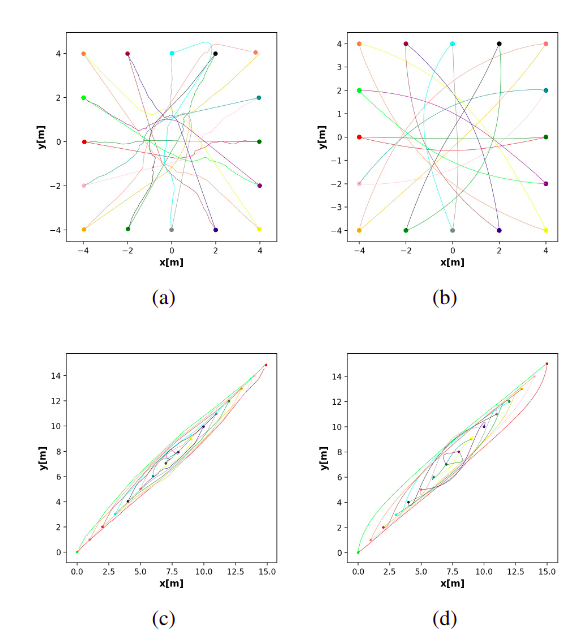
\includegraphics[scale=0.6]{figures/appendix/RVO_inits.png}} 
    \caption[Appendix: Trajectories using RVO + multi-robot optimizer]{Comparison of trajectories from a) RVO alone in 16 Robots 2D Square Antipodal b) Optimizer + RVO initialization for 16 Robots 2D Square Antipodal c) RVO alone in 16 Robots 2D Ellipse b) Optimizer + RVO initialization for 16 Robots 2D Ellipse.}
    \label{fig:RVO+opti_2D}
\end{figure}

\section{Initializations using Multi-robot Pathfinding(MAPF)\cite{sharon_journal}}\label{sec:appendix-MAPF}

Similar to RVO, we can also couple graph-search-based Multi-robot Pathfinding (MAPF) algorithms discussed in Section \ref{sec:MAPF} for initializing our optimizer. For this purpose, we will use the \texttt{cbs-mapf} PyPI package that implements the high-level Conflict Based Search Algorithm based on \cite{sharon_journal} and low-level space-time A*(STA*), which is similar to normal A*(from Section \ref{sec:A*} with an additional time dimension. The trajectories generated by CBS-MAPF are piecewise linear and exhibit jerks and sharp turns, so these cannot be used practically for multi-robot navigation. We scale up the start and goal coordinates depending on grid size (we use grid size = 10) as well as the robot radii and precompute multi-robot trajectories using CBS-MAPF. Similar to the RVO trajectories, we sample points from the trajectories obtained from CBS-MAPF to calculate the optimizer parameters and initialize our optimizer. 

We introduce a new scenario to test MAPF for 14 Robots arranged in a 2D grid and are needed to move to the opposite end of the grid. Figure \ref{fig:MAPF+opti_grid} shows a comparison of trajectories between CBS-MAPF alone and the optimizer using CBS-MAPF for initialization. We again observe a significant improvement in the smoothness of the trajectories generated by our optimizer with CBS-MAPF initialization compared to CBS-MAPF alone. However, similar to RVO, there is no benefit to using MAPF initialization in terms of computational time. 

\begin{figure}[H]
    \centering
    {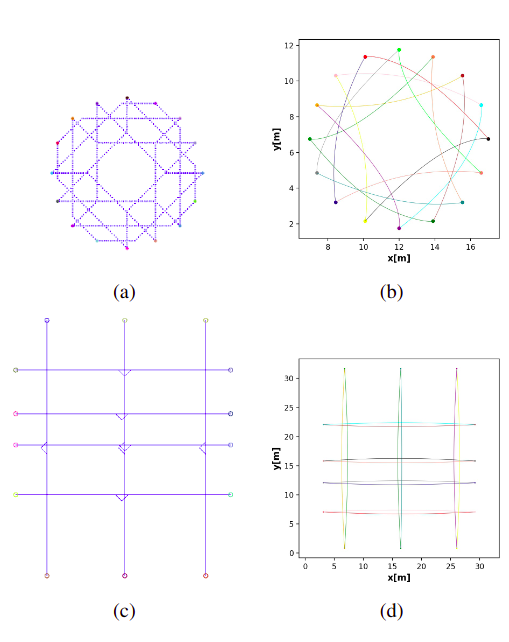
\includegraphics[scale=0.6]{figures/appendix/mapf_init.png}} 
    \caption[Appendix: Trajectories using MAPF + multi-robot optimizer]{Comparison of trajectories generated by CBS-MAPF alone and our optimizer with CBS-MAPF initialization for a)-b) 16 Robots in the Circle(k=5) scenario, c)-d) 14 Robots in 2D Grid orientation.}
    \label{fig:MAPF+opti_grid}
\end{figure}

%--------------------------------------------------------
% Recommended 'Related Publication'
\chapter*{Related Publications}
\label{ch:relatedPubs}
\begin{enumerate}
    \item Guhathakurta, D., Rastgar, F., Sharma, M. A., Krishna, K. M., \& Singh, A. K. (2022). Fast Joint Multi-Robot Trajectory Optimization by GPU Accelerated Batch Solution of Distributed Sub-Problems. \textit{Frontiers in Robotics and AI, 9}. doi:10.3389/frobt.2022.890385
    
    \item Guhathakurta, D., Rastgar, F., Sharma, M. A., Krishna, M., \& Singh, A. K. (2022). GPU Acceleration of Joint Multi-Agent Trajectory Optimization. Poster presented at IROS 2022 workshop on \textit{Decision Making in Multi-Agent Systems(DMMAS)}, Kyoto, Japan.
\end{enumerate}



%--------------------------------------------------------

\bibliographystyle{unsrt}
\bibliography{
    bibliography/main,
    bibliography/gpu_mat,
    bibliography/manipulator
} 

\end{document}
